 %% ----------------------------------------------------------------
%% Thesis.tex -- MAIN FILE
%% Gao Rui
%% work on AUV positioning
%% ----------------------------------------------------------------

\documentclass[a4paper, 12pt, oneside]{Thesis}

% Include any extra LaTeX packages required
%\usepackage[inner=2.5inch,outer=1.5inch,bottom=1inch]{geometry}
\usepackage{setspace}
\doublespacing
\usepackage[square, numbers, comma, sort&compress]{natbib}  % Use the "Natbib" style for the references in the Bibliography
\usepackage{verbatim}       % Needed for the "comment" environment to make LaTeX comments
\usepackage[utf8]{inputenc}
\usepackage[english]{babel}
\usepackage{vector}
\usepackage{amsmath}
 {
      \theoremstyle{plain}
      \newtheorem{assumption}{Assumption}
  }
\usepackage{subfigure}
\usepackage{setspace}
\usepackage{graphics}
\usepackage{graphicx}
\usepackage{textcomp}
\usepackage{multirow}
\usepackage{array}
\usepackage{tikz} % PGF
\usepackage{enumerate}
\usepackage{float}
\usepackage{rotating}
\usepackage{subfigure}
\usepackage{algorithm2e}
\usepackage{algorithm}
\usepackage[utf8]{inputenc}
%\usepackage[ngerman, english]{babel}
\usepackage{csquotes}
\usepackage{hyperref}
\usepackage{xcolor}
\newcommand{\cbox}[2][yellow]{%
  \colorbox{#1}{\parbox{\dimexpr\linewidth-2\fboxsep}{\strut #2\strut}}%
}
\hypersetup{
    colorlinks=true,
    linkcolor=blue,
    filecolor=magenta,      
    urlcolor=cyan,
}
\graphicspath{{./Figures/}}       % (set up for graphics to be in PDF format)

\hypersetup{linkcolor=black, colorlinks=true, citecolor = black} % Colours hyperlinks in blue, but this can be distracting if there are many links.
\urlstyle{same}
%\hyphenation{STARFISH AUVs}

\pagestyle{plain}
%% ----------------------------------------------------------------
\begin{document}


\frontmatter        % Begin Roman style (i, ii, iii, iv...) page numbering

\title      {COOPERATIVE LOCALIZATION AND BATHYMETRY-AIDED NAVIGATION OF AUTONOMOUS MARINE SYSTEMS }\\
%% FINAL 

\authors    {GAO RUI}

\maketitle

    \chapter*{\centering Declaration}
\addcontentsline{toc}{chapter}{Declaration}
\begin{center}

I hereby declare that this thesis is my original work and it has been written by me in its entirety. I have duly acknowledged all the sources of information which have been used in the thesis.

This thesis has also not been submitted for any degree in any university previously.


\vspace{20mm}  % vertical space

\rule{40mm}{.15mm}\par   % horizontal space, line, start new line
 Gao Rui\par
\today
\end{center}


\clearpage
\lhead{\emph{Acknowledgements}} 
\acknowledgements{
\addtocontents{toc}{\vspace{1em}}       % Add a gap in the Contents, for aesthetics
This dissertation would not be possible without the assistance of many people. I am very fortunate to be associated with them and would like to take this opportunity to express my gratefulness and appreciation to them in this acknowledgement.

First and foremost, I would like to thank my supervisor Assoc.~Prof.~Mandar~Chitre who introduced me to underwater navigation. He not only provided the patient guidance and valuable suggestions but more importantly supported and encouraged me throughout the course. He has my utmost respect and gratitude for understanding and believing in me, especially when I was overwhelmed with my family commitment. 

This dissertation was built on the project - STARFISH AUV\footnote{Small Team of Autonomous Robotic ``Fish'' (STARFISH)} at ARL\footnote{Acoustic Research Laboratory (ARL), Tropical Marine Science Institute (TMSI), National University of Singapore (NUS) - \url{http://www.arl.nus.edu.sg}}, NUS. I would like to extend my gratitude to my colleagues and friends at ARL. I am grateful for the opportunity for working with and being surrounded by great people. I am honored to be part of an outstanding team. Thanks go to Ms.~Ong~Lee~Lin for her help and guidance in my research writing.

Last but not least, I want to thank my husband, Chew~Jee~Loong, and my loving parents. This journey would not have been possible without their understanding and support. My deepest gratitude goes to my dear mother for her unconditional love, encourage, and all the sacrifices she has made for me. I shall also mention my two kids, Amelie and Andrew, who always make my day full of joy and happiness.
}
\lhead{\emph{Acknowledgements}} 
\clearpage      % End of the Acknowledgements
%% ----------------------------------------------------------------
\pagestyle{fancy}       %The page style headers have been "empty" all this time, now use the "fancy" headers as defined before to bring them back


%% ----------------------------------------------------------------
\setcounter{tocdepth}{2}
\lhead{\emph{Contents}}     % Set the left side page header to "Contents"
\tableofcontents        % Write out the Table of Contents

% -------------------------The Abstract Page-------------------------
\addtotoc{Summary}     % Add the "Abstract" page entry to the Contents
\lhead{\emph{Summary}} 
\abstract{
\addtocontents{toc}{\vspace{1em}}       % Add a gap in the Contents, for aesthetics

In monitoring and surveillance, localization and navigation is especially important for underwater autonomous vehicles (AUVs) since GPS and radio signals are not accessible in most of the missions. A cooperative team formed by multiple autonomous vehicles has gained increasing interests as it offers more efficiency and reliability than a single vehicle. Much work has been done in the area of underwater localization and navigation with the aids from beacons with known positions. This dissertation focuses on a team of low-cost AUVs where no one has precise position. With the ability to communicate and make relative measurements from each other, vehicles share information across the team and cooperate to complete complex missions. The information shared among vehicles helps improve the overall performance. However, unlike terrestrial communication links, underwater acoustic channel has inherent constraints such as high latency, limited bandwidth and low reliability. In such a case, a distributed processing architecture with minimum inter-vehicle communications is preferred. At the same time, the severe underwater communication issues also impose challenges on the distributed processing. We show the benefit introduced through cooperation and the issue imposed by communication constraints on the distributed processing. We propose a feasible design of the distributed localization for a team of cooperative AUVs. The algorithm is robust to packet loss, outperforms single-vehicle localization and requires minimum communications. 

In the next step, we look at a simplified \textit{na\"ive} assumption in underwater multi-sensor tracking and multi-vehicle localization. This assumption \textit{na\"ively} assumes information from different sources are independent of each other. We justify the assumption and answer when the assumption is good to use. With the justification, we move on to single-vehicle bathymetry-aided navigation as it can be safely extended to cooperative multi-vehicle navigation with bathymetric aids. 

Bathymetry map indicating the water depth offers an attractive tool to reduce the localization error of the submerged vehicles. With bathymetric measurements incorporated, we study the \textit{a posteriori} description of the localization uncertainty using probabilistic methods. An information theoretical approach is used to describe the localization uncertainty. With this information theory measure, we build information entropy map and demonstrate how the bathymetry helps with different localization priors. Subsequently, a bathymetry-aided navigation is proposed to ensure a good localization at the destination. We formulate the path planning and solve it as an optimization problem. The algorithm is tested using real-world bathymetric data. Simulations show that near-optimal paths with good localization accuracy at the destination are generated within a few iterations.

\clearpage      % Abstract ended, start a new page
% ------------------------------------------------------
\lhead{\emph{List of Tables}}       % Set the left side page header to "List of Tables"
\listoftables       % Write out the List of Tables

% --------------------------------------------------
\lhead{\emph{List of Figures}}      % Set the left side page header to "List if Figures"
\listoffigures      % Write out the List of Figures

%% ----------------------Symbols---------------------------
\clearpage      %Start a new page
\lhead{\emph{List of Symbols}}      % Set the left side page header to "Symbols"
\listofnomenclature{ll}        % Include a list of Symbols (a three column table)
{
 $k$ & time step $k$, used as subscript for other symbols \\
${\bf x}_k$ & position state at time step $k$ \\
${\bf a}_k$ & action directing vehicle movement at time step $k$ \\
${\bf F}$ & Jacobian matrix of evolution model \\
${\bf H}$ & Jacobian matrix of measurement model \\
${\bf B}_k$ & control matrix at time step $k$\\
${\bf u}_k$ & control input at time step $k$\\
${\bf z}_k$ & measurement or observation at time step $k$ \\
${\bf Z}_{1:k}$ & series of measurements from time step 1 to $k$ \\
$r_k$ & range measurement at time step $k$ \\
${\bf\omega}_k$ & system evolution noise \\
${\bf Q}_k$ & covariance of system evolution noise \\
${\bf\nu}_k$ & measurement noise \\
${\bf\upsilon}_k$ & range measurement noise \\
${\bf R}$ & covariance of measurement noise \\
${\bf R}_r$ & covariance of ranging error \\
${\bf\hat x}_k,{\bf y}_k$ & position estimate of true position state ${\bf x}_k$ \\
${\bf P}_k$ & error covariance of the position estimate\\
$\delta T$ & measurement update interval \\
$p_L$ & communication packet loss rate\\
$N_p$ & number of past updates \\
${{\Lambda}}_k$ & precision matrix or information matrix\\
${\bf \eta}_k$ & information vector \\
${\bf O}_{\bf x}$ & State mapping matrix \\ 
${\bf O}_{\bf y}$ & Observation mapping matrix\\ 
 ${\bf E}$ & Error matrix\\
}

%% ----------------------------------------------------------------
%\setstretch{1.5}        % Set the line spacing to 1.5, this makes the following tables easier to read
\clearpage      % Start a new page

%% ----------------Abbreviations---------------------------
\lhead{\emph{Acronyms}}        % Set the left side page header to "Abbreviations"
\listofsymbols{ll}      % Include a list of Abbreviations (a table of two columns)
{
\textbf{AUV} & \textbf{A}utonomous \textbf{U}nderwater \textbf{V}ehicle \\
\textbf{BAN} & \textbf{B}athymetry \textbf{A}ided \texbf{N}avigation \\
\textbf{CKF} & \textbf{C}entralized \textbf{K}alman \textbf{F}ilter \\
\textbf{DF} & \textbf{D}istributed \textbf{F}ilter \\
\textbf{DoF} & \textbf{D}egree-\textbf{o}f-\textbf{F}reedom \\
\textbf{DR} & \textbf{D}ead \textbf{R}eckoning \\
\textbf{DVL} & \textbf{D}oppler \textbf{V}elocity \textbf{L}og \\
\textbf{EKF} & \textbf{E}xtended \textbf{K}alman \textbf{F}ilter \\
\textbf{EIF} & \textbf{E}xtended \textbf{I}nformation \textbf{F}ilter \\
\textbf{GIB} & \textbf{G}PS \textbf{I}ntelligent \textbf{B}uoys\\
\textbf{GMM} & \textbf{G}aussian \textbf{M}ixture \textbf{M}odel \\
\textbf{INS} & \textbf{I}ntertial \textbf{N}avigation \textbf{S}ystem \\
\textbf{KF} & \textbf{K}alman \textbf{F}ilter \\
\textbf{LBL} & \textbf{L}ong \textbf{B}ase \textbf{L}ine\\
\textbf{MAP} & \textbf{M}aximum \textbf{A} \textbf{P}osteriori \\
\textbf{ML} & \textbf{M}aximum \textbf{L}ikelihood \\
\textbf{NEES} & \textbf{N}ormalized \textbf{E}stimation \textbf{E}rror \textbf{S}qaured \\
\textbf{NKF} & \textit{\textbf{N}a\"ive} \textbf{K}alman \textbf{F}ilter \\
\textbf{PDF} & \textbf{P}robabilistic \textbf{D}ensity \textbf{F}unction \\
\textbf{PF} & \textbf{P}article \textbf{F}ilter \\
\textbf{PV} & \textbf{P}eer \textbf{V}ehicle \\
\textbf{RMSE} & \textbf{R}oot \textbf{M}ean \textbf{S}quare \textbf{E}rror \\
\textbf{RV} & \textbf{R}eceiving \textbf{V}ehicle \\
\textbf{(U)SBL} & (\textbf{U}ltra) \textbf{S}hort \textbf{B}ase \textbf{L}ine\\
\textbf{SCI} & \textbf{S}plit \textbf{C}ovariance \textbf{I}ntersection \\
\textbf{SI} & \textbf{S}warm \textbf{I}ntelligence \\
\textbf{SPP} & \textbf{S}elf-\textbf{P}ropelled \textbf{P}articles \\
\textbf{SVF} & \textbf{S}tate \textbf{V}ector \textbf{F}usion \\
}

%%% -------------------Physical Constants----------------------------
%\clearpage      % Start a new page
%\lhead{\emph{Physical Constants}}       % Set the left side page header to "Physical Constants"
%\listofconstants{lrcl}      % Include a list of Physical Constants (a four column table)
%{
% Constant Name & Symbol & = & Constant Value (with units) \\
%Speed of Sound in Seawater & $c$ & $=$ & 1540\ m s$^{-1}$ \\
%}




%% ----------------------------------------------------------------
% End of the pre-able, contents and lists of things
% Begin the Dedication page

\setstretch{1.3}        % Return the line spacing back to 1.3


%% ----------------------------------------------------------------
\mainmatter     % Begin normal, numeric (1,2,3...) page numbering
\pagestyle{fancy}       % Return the page headers back to the "fancy" style

% Include the chapters of the thesis, as separate files
% Just uncomment the lines as you write the chapters
\setstretch{2}        % Return the line spacing back to 1.3

% Chapter 1

\chapter{Introduction}
\label{ch:introduction}
\lhead{Chapter~\ref{ch:introduction}. \emph{Introduction}}

\section{Motivation}
\label{sec:Motivation}

The past decade has seen a significant increase in interest in the use of autonomous underwater vehicles (AUVs) for maritime operations. AUVs reach shallower water than boats, and greater depths than human divers or tethered vehicles. Once deployed and submerged, AUVs are safe from bad weather and heavy traffic on the surface. Extensive research has been conducted on AUVs and several commercial AUVs have been developed and tested \cite{Kojima1997,Hagen2006,Byron2007}. One of the challenges that all AUVs have to contend with is that of underwater localization and navigation, since GPS signals cannot be received underwater. For missions such as mapping, target identification, sensing and surveying, underwater localization and navigation are the key components that determine the performance of an autonomous mission. 

Traditionally an AUV localizes itself using the vehicle's own sensor data, such as GPS (whenever available), compass and depth sensor. In order to obtain good localization, AUVs are often equipped with high-end navigation systems such as Doppler velocity log (DVL) and inertial navigation system (INS). Packed together with other sensors for the mission (for example, sensors for monitoring and surveying), AUVs become bulky in size and high in cost. Another way to achieve the vehicle's localization accuracy is to utilize the communication with beacons with known positions. The distance from AUV to a beacon can be measured by the time-of-flight (TOF) of the acoustic signals. The relative orientation of the AUV can be computed from a set of equations consisting of distances to all available beacons \cite{Zhou} or the phase shift measured from the beacon array \cite{Marin2018}. Long Baseline (LBL) uses a sea-floor baseline transponder network as navigation reference. It gives very high positioning accuracy and position stability, but incurs high effort and cost to deploy and support this substantial infrastructure. Other techniques such as Short Baseline (SBL), Ultra Short Baseline (USBL) \cite{milne1983} and GPS Intelligent Buoys (GIB) \cite{Alcocer2006} are placed on sea surface. Localization with these setups can only be achieved in certain restricted and designated areas due to the installation of these external beacons. Some systems also assist the localization and navigation with moving beacons such as those mounted on surface vessels \cite{Webster2013,AlexPhillips2018,Giovanni2018} or even other AUVs \cite{Gao2010}. The operation of additional surface vessels is not trivial; the horizontal coverage is also limited. The positions of beacon AUVs need to be calibrated precisely. 

In these respects, AUVs which are able to navigate without aids from external setups or beacons and yet still maintain good localization with the use of low-grade sensors, are preferred. This has motivated multi-vehicle localization and navigation \cite{Martins2003,Busquets2012,Gao2010}, and the use of bathymetric aids. 

Multi-vehicle operation offers robustness to single-vehicle failure and reduces the overall time and cost of acquiring data over large areas. We focus on a team of low-cost AUVs where no single AUV functions as a beacon possessing accurate position. The team is able to outperform single-vehicle operation, through sharing information among the team members. However, as compared to terrestrial communication links, underwater communication links typically are encumbered by limited bandwidth, high latency and significant packet loss. It is impractical for a team of AUVs to collate all sensor data centrally, and therefore a decentralized processing architecture is preferred. However this opens up new challenges to team members working in cooperation.

The first challenge lies in the limited communication bandwidth. As mentioned, the multi-vehicle localization problem consists of a team of vehicles cooperating and estimating their own positions. If the local sensor data are accessible to a central processing unit, a central filtering yields the optimal estimation on all vehicle positions. However, with limited bandwidth, the size of underwater transmission packets is constrained. The information shared between members is usually processed estimates rather than the raw sensor data. A distributed filtering where members only process their local sensor data and information communicated from others is commonly used. An empirical study~\cite{William2015Journal} showed that the available bandwidth in underwater communication severely limits the performance of cooperative localization.

The second challenge pertains to tracking of the inter-vehicle correlation. In the presence of unstable, irregular and lossy channels, the information exchange between two vehicles may not be known to other members in the team. Therefore the inter-vehicle correlation tends to be underestimated. A common practice is to \textit{na\"ively} assume independence during information fusion between cooperative members. This assumption is not always good. Overconfidence in estimation has been reported as a result of double counting the common information \cite{Julier2001book}. This overconfidence prevents utilization of subsequent useful measurements. To prevent information double counting, author in \cite{BahrThesis} selectively incorporated information and avoided the fusion of correlated data while keeping the positions of all vehicles decorrelated. Other works assumed maximum correlation in the whole state~\cite{Uhlmann2003,Benaskeur2002,Yan2008} or separated states~\cite{LiHao2013B}. These methods are conservative in handling the unknown inter-vehicle correlation, and typically yield pessimistic estimates as the independent information is not fully utilized. Based on the way that vehicles cooperate, a less conservative distributed localization could be designed to record the correlated terms and require minimum communications. Meanwhile, the \textit{na\"ive} assumption which simply ignores the correlation, has been used as a common practice as it imposes minimum requirements on the processing and communication. One would be interested to know how information double counting happens and when the correlation in fusion can be ignored. The dangerous and safe regions of \textit{na\"ive} filtering should be quantified.

Incorporating information sensed from the natural environment helps improve the localization without the need to establish extra physical infrastructure. Bathymetry map indicating the water depth offers an attractive tool to reduce the localization error of the submerged vehicles. Reference \cite{William2015Journal} presents a cooperative bathymetry-based localization approach for a team of low-cost AUVs. It presents empirical analysis on the factors that affect the filter performance. However, vehicle estimates are assumed to be independent of each other as the author claims that the effect of correlation is alleviated with bathymetry measurements. The amount of common information fed back through the cooperation in the team is not addressed. In our work, we justify this assumption through a careful analysis of the effect of bathymetry aids in navigation. The advantage of bathymetric aids is path dependent. It makes sense if vehicles are able to plan a path such that a good localization can be ensured. It is generally believed that localization performance depends on the rugosity of the sea bottom. Authors in \cite{Kalyan2013} show that the bathymetry variation is closely related to the localization performance. Bathymetry variation is commonly used to guide vehicles towards maximizing the bathymetric aids on localization. In~\cite{Galceran2013}, heuristics were used to visit salient points (locations with more bathymetric variation) for better localization. In~\cite{Peng2016}, terrain dispersion, roughness and terrain entropy were evaluated. However, the waypoints along the path were selected manually. In \cite{Rodrigo2015}, trajectories were generated by guiding vehicles to avoid areas with smooth sea floor. In order to plan a path to maximize the effect of bathymetric aids, we need to understand what kind of bathymetry make good localization first. Is the bathymetry variation the sufficient condition? How does one define a good localization? With these answers, we propose a path planning algorithm to optimize the localization performance with bathymetric aids.

\section{Thesis Contribution and List of Publications}
\label{sec:Publication}
% bullet form

This thesis presents our work on cooperative localization and bathymetry-aided navigation of autonomous marine systems, with AUVs being the particular focus. The key contributions of this thesis are listed below:
\begin{enumerate}
    \item {Distributed localization is explored 
using a cooperating team of small-sized, low-cost, sensor-limited AUVs. In the presence of underwater communication challenges, we found that localization easily deteriorate when communication loss is high.}
    \item A new cooperative multi-vehicle localization algorithm using distributed extended information filter (DEIF) is proposed. The proposed method is effective in recording the correlated information in light of constrained underwater communication.
    \item {We answer the question as to when the correlation can be safely ignored. The safe and dangerous regions for implementation of \textit{na\"ive} filtering in decentralized architecture are derived for multi-sensor tracking problem and multi-vehicle localization problem. The link between these two problems is explained with formulations.}
    \item We formalize a concept of an information entropy map to quantify the effectiveness of bathymetry measurements on localization.
    \item A path planning algorithm is proposed for navigation with bathymetric aids. The algorithm generates near-optimal paths based on bathymetric maps, with good localization accuracy generated at the destination.  
\end{enumerate}

\section{Related Publications}
\begin{enumerate}[ {[}1{]} ]
\item R. Gao and M. Chitre, ``Bathymetry-aided Navigation of Autonomous Underwater Vehicles (AUVs)'', Manuscript in preparation for IEEE Journal of Oceanic Engineering
     \item R. Gao and M. Chitre,``Path Planning for Bathymetry-aided Underwater Navigation,'' in Autonomous Underwater Vehicles (AUV 2018), (Porto, Portugal), November 2018.
    
    \item R. Gao and M. Chitre, ``On distributed processing for underwater cooperative localization,'' in 14th International Conference on Ubiquitous Robots and Ambient Intelligence (URAI 2017), (Jeju, South Korea), July 2017. (Invited).
    
    \item R. Gao and M. Chitre, ``Cooperative Multi-AUV localization using distributed extended information filter,'' in Autonomous Underwater Vehicles (AUV 2016), (Tokyo, Japan), pp. 206--212, November 2016.
\end{enumerate}

\section{Thesis Layout}
\label{sec:Layout}
% thesis organization

This thesis is organized as follows.

Chapter~\ref{ch:background} provides a brief discussion of related works in cooperative localization and bathymetry-aided navigation. Chapter~\ref{ch:distributed} presents the decentralized processing when vehicles cooperate with communication constraints. A novel distributed localization method is proposed. Chapter~\ref{ch:naive} answers the question of when the correlation can be safely ignored when fusing estimates from different sources. The safe and dangerous regions of implementing \textit{na\"ive} filtering (ignoring correlation) are derived in two applications. The bathymetry-aided localization is justified to be safe if correlation is ignored in cooperation.

Chapter~\ref{ch:bathymetry} illustrates localization with bathymetric aids using an information theoretic approach. In light of the entropy measure and the relation to localization introduced in Chapter~\ref{ch:bathymetry}, a path planning algorithm is proposed and tested through simulation in Chapter~\ref{ch:ban}. 

Chapter~\ref{ch:conclusion} summarizes the key findings in the research and makes suggestions for future works.



   





 % 1.Introduction
% Chapter 2

\chapter{Background}
\label{ch:background}
\lhead{Chapter~\ref{ch:background}. \emph{Background}}

%\section{Underwater Localization}

\section{AUVs and Localization}

The words \textit{Positioning} and \textit{localization} are often used interchangeably in literature. Positioning, although similar to localization, also has the connection of placing the vehicle in a particular place. In this thesis, we will use the word \textit{localization} to mean the process of locating the vehicle, with or without the reference of a map.

The sensors for underwater localization are categorized into two groups. The first group of sensors do not require external infrastructure for localization. For example, DVL measures vehicle speed relative to the seabed. A microelectromechanical system (MEMS), usually called as compass, measures the vehicle's 3-axis orientation. An inertial measurement unit (IMU) provides the vehicle's acceleration and angular rate with respect to the vehicle's body-frame. Other examples include depth sensor, altimeter, sidescan sonar, and forward looking sonar (FLS). Localization by these sensors usually observe the natural environment as external references and can be performed in any environment. However these sensors often do not give full information about vehicle's location. The most common localization method of localization with these sensors is dead reckoning (DR). It calculates the vehicle's position by integration of velocity over time. Accurate DR systems tend to be expensive as high-grade sensors are needed. Even though, any small bias or offset leads to an unbounded increase in error over time while AUV remains submerged. The second group are sensors which require additional infrastructure setup. Acoustic positioning systems measure vehicle's range and/or angle to the beacons and therefore provide direct estimates of the position relative to beacons. The beacons can be fixed to sea bottom, or the surface vehicles, or even other AUVs. These sensors give good localization reference but often incurs high cost in deployment and operation.

In a typical localization problem, the state to be estimated usually consists of the vehicle's position, depth, orientation (heading, pitch and roll) and velocity. During a mission, the autonomous vehicle estimates its own state and at the same time uses the estimated state for further actions. Usually the depth of an AUV is specified in a mission and measured by the depth sensor directly. Therefore in this thesis we only focus on the vehicle's position in the 2-dimensional space, that is, the northing-easting position.

Let ${\bf x}_k$ be the state vector to be estimated at time step $k$ where ${\bf x}_k\in\mathbb{R}^n$, and let the estimate of ${\bf x}_k$ be ${\bf \hat x}_k$ (In some illustration in this thesis, we also use ${\bf y}_k$ to denote the estimate of state ${\bf x}_k$).  The general system evolution is modeled as
\begin{equation}
\label{eq:propagation}
{\bf x}_{k+1}=f({\bf x}_k,{\bf a}_k)+{\bf\omega}_k
\end{equation}
where ${\bf a}_k$ is the action that directs vehicle movement for the next step. The behavior of the system is observed through measurement ${\bf z}_k\in\mathbb{R}^m$. The measurement model is
\begin{equation}
\label{eq:measurement}
{\bf z}_{k+1}=h({\bf x}_{k+1})+{\bf\nu}_{k+1}.
\end{equation}
The process noise ${\bf\omega}_k$ and measurement noise ${\bf\nu}_k$ are Gaussian white-noise sequences and are mutually independent. Their error covariances are ${\bf Q}_k$ and ${\bf R}_{k+1}$ respectively.

Typically the vehicle carries a belief as to where it might be, and maintains the localization as a probability distribution over the space of all such hypotheses. Knowledge of the probability density function (PDF) of the state conditioned on all available measurement data ${\bf Z}_{1:k}\triangleq\{{\bf z}_1,{\bf z}_2,...,{\bf z}_k\}$ provides the most complete possible description of the state. Given \textit{a posteriori} density function $p({\bf x}_k|{\bf Z}_{1:k})$, estimate ${\bf \hat x}_k$ of the state is obtained from some performance criteria, for example, maximum \textit{a posteriori} (MAP). Bayesian estimation \cite{Aoki1967} recursively determines the a posteriori density $p({\bf x}_k|{\bf Z}_{1:k})$ as
\begin{align}
\begin{split}
p({\bf x}_k|{\bf Z}_{1:k})&=\frac{p({\bf z}_{k}|{\bf x}_k)p({\bf x}_k|{\bf Z}_{1:k-1})}{p({\bf z}_k|{\bf Z}_{1:k})} \\
&=\alpha p({\bf z}_{k}|{\bf x}_k)p({\bf x}_k|{\bf Z}_{1:k-1}) \\
\end{split}
\end{align}
where
\begin{align}
\begin{split}
\frac{1}{\alpha}&\triangleq p({\bf z}_k|{\bf Z}_{1:k}) \\
&=\int p({\bf z}_{k}|{\bf x}_k)p({\bf x}_k|{\bf Z}_{1:k-1})\mathrm{d}{\bf x}_{k}.
\end{split}
\end{align} % wiki recursive bayesian estimation
The simplification is based on Markov assumption \cite{Alspach1972} which states that if one knows the vehicle location ${\bf x}_k$, future measurements are independent of the past ones, that is
\begin{equation}
    p({\bf z}_k|{\bf x}_k,{\bf Z}_{1:k-1})=p({\bf z}_k|{\bf x}_k).
\end{equation}
The density $p({\bf z}_{k}|{\bf x}_k)$ is the \textit{a priori} distribution describing the sensor model. The state transition model is described by the prediction as
\begin{equation}
p({\bf x}_k|{\bf Z}_{1:k-1})=\int p({\bf x}_{k}|{\bf x}_{k-1})p({\bf x}_{k-1}|{\bf Z}_{1:k-1})d{\bf x}_{k-1}.   
\end{equation}

When both evolution and measurement models are linear with additive Gaussian noises, and the \textit{a priori} distribution is Gaussian, Kalman filter (KF) \cite{welch1995} can be used to derive the closed-form solution by simply using the estimated mean ${\bf\hat x}$ and estimated covariance ${\bf P}$ for this system. The parametric description of the distribution is efficient in integrating the motion and updating the estimates, and also easy to evaluate the localization performance. However it is only suitable for linear systems with Gaussian noises. Extended Kalman filter (EKF) \cite{Julier2004} is the nonlinear version of the KF which linearizes the nonlinear evolution and/or nonlinear measurements. Only unimodal distributions can be modeled by KF and its extensions. Nonparametric filters use numerical approaches to describe the PDF and are particularly suitable for nonlinear and non-Gaussian system estimation since their probability function evolves to better fit the data. The most well-known nonparametric method is the Particle filter (PF) \cite{PFtutorial}.

\section{Beacon-Based Localization}

In beacon-based localization, beacons are placed in the area where AUVs navigate. For example, long baseline acoustic positioning system (LBL) places the transponders on the seafloor, while short baseline system (SBL) and ultra short baseline system (USBL) have the transponders mounted on a ship that follows the vehicle. These methods differ in the distances between the transponders and the distance from each transponder to the vehicle \cite{Wolbrecht2014}. The GIB system uses buoys on the surface \cite{Alcocer2006}. When fixed beacons are used \cite{AlexPhillips2018B}, AUVs are limited in their exploration area. The deployment and setup of the infrastructure are tedious and expensive. Some systems assist the localization with moving beacons. The moving beacons can be mounted on vessels \cite{Curcio2005, Webster2013,AlexPhillips2018} or even other AUVs \cite{Baccou2001,Deshpande2007,Gao2010}. Surface vessels often encounter danger of collision with other traffic on the surface.
Beacon AUVs are usually assumed to have precise positioning. Generally the beacon vehicle operates at the surface and has access to GPS, or is equipped with high-accuracy sensors which enables it to estimate its own position with minimum errors. A setup, which consists of beacon AUVs with precise positioning, can form a cooperative team of heterogeneous AUVs. 

\section{Cooperative Localization}

The idea of cooperative localization with beacon AUV is not new.
Authors in \cite{Gao2010,William2014Journal} presented a single-beacon vehicle providing range-only measurement to support the localization of other AUVs. The supported AUVs are survey AUVs equipped with sensors for mission purposes. For example, LEDIF sensor \cite{NgLEDIF} was installed on STARFISH AUVs \cite{STARFISH} for chemical sensing. With these sensing units, survey AUVs are often equipped with poor navigation sensors. The distance between the survey AUV and the beacon vehicle is measured to impose a limit on the position drift of the survey AUV. This approach has been explored by several works which use observability analysis \cite{Antonelli2010,Song1999}, and position determination algorithms \cite{Gadre2004,Alleyne2000}. However, these works pay little attention to the path planning of the beacon vehicle. For example,  \cite{Alleyne2000} assumed a circular path for the beacon vehicle, \cite{Fallon2010} used a zigzag path during experiments and \cite{Webster2012} adopted a diamond shaped path.

It is acknowledged that the relative motion between the beacon vehicle and the survey AUVs is key to having single beacon range-only navigation perform well. The path of the beacon vehicle should be planned in such a way that it improves the position estimate of the survey AUVs. In \cite{chitre2010}, the path planning of the beacon vehicle aimed at minimizing the accumulated localization errors in the supported survey AUVs. In \cite{Bahr2009beacon}, the optimal beacon point targeted at minimizing the position uncertainty of the survey AUV, but it was determined by brute-force searching approach. Later \cite{William2014Journal} proposed the cooperative path planning algorithm using dynamic programming and Markov decision process formulations.

In the waters of Singapore, heavy maritime traffic makes it dangerous and inconvenient for AUVs to surface for GPS fix. Consequently, even beacon AUVs with high-grade sensors suffer from position drift. We look at this problem and propose a solution whereby no single AUV functions as a beacon possessing accurate position information in the team. In terms localization capability, the team of AUVs is a homogeneous team, whereas a heterogeneous team includes a beacon AUV with precise position. The relative position or range between these AUVs can be considered as a relative geometry constraint in
localization. This cooperative localization is easier to be understood if we treat the group of AUVs as one identity. The individual AUVs are the multiple ``limbs" while the distances between AUVs are the multiple virtual ``joints". Each limb moves on its own path, and from time to time, when the distance between two AUVs is measured, the position estimates of all the AUVs are
adjusted accordingly. Cooperative multi-AUV localization has the potential to outperform single-AUV localization, by taking advantage of data sharing among the team members. However, it should be noted that many factors affect the communication and subsequently the cooperation performance. Water temperature, salinity, underwater noise, Doppler phase shift, reflection and scattering of seabed and sea surface are relevant contributing factors to be considered. Underwater communications have limited bandwidth and are less reliable compared with terrestrial communication links. Full
communication with every member of the team at any one time of instant is often not practical.

In such a case, decentralization in processing and navigation becomes necessary. One example of decentralized processing comes from the self-organized behavior, namely \textit{Swarm Intelligence (SI)}. SI system consists of a population of simple agents, which interact locally with one another following simple rules. There is no centralized unit or individual who knows the full details or dictates how each member should behave. Interactions between agents lead to an ordered or ``intelligent'' global behavior. The phenomenon is often referred to as `emergence'.  The inspiration often comes from nature, especially biological system behavior like ant colonies, bird flocking, animal herding and fish schooling. The application of
SI to robotics is called `swarm robotics', a method of coordinating large numbers of simple robots, which interact with one another to give rise to a desired collective behavior \cite{SI1,SI2,SI3}. In ocean studies, the use of swarm AUVs for data gathering purposes has emerged as an attractive and alternative solution to the tedious and manual process of deploying sensor probes, for example beacons installed on surface vessels. Swarm AUVs are able to gather more data than the traditional approach, operating at lower overall cost, and can be deployed to function in harsh environment. It is also robust to individual failure, compared with the single-AUV system. Swarm AUVs
coordinate their behavior in a distributed way to achieve a particular goal, such as resource sharing, synchronized motion \cite{Sam2005}, localization \cite{liu2014}, a specific swarm pattern or coverage \cite{Spires1998}, etc.

The concept of SI can be visualized in the tutorial about self-propelled particles (SPP) in \cite{Sam2005}. In this tutorial, each particle has its own randomness in movement and follows the average heading when it meets other particles within its vicinity. It introduces order parameters and other critical values to visualize how the order or phase change with respect to the variation of randomness, number of particles, vicinity range etc. In SI, the communication and coordination among members is usually minimal. The observation on other members also comes with more randomness.

\section{Dealing with Unknown Correlation}
\label{sec:unknowncorrelation}
In this thesis, we focus on a small team of AUVs. These AUVs locally estimate their own positions, and gather observations to update the position estimates. The distributed processing architecture has many advantages over centralized architecture. It is reliable in the sense that the loss of any individual AUV or links does not necessarily prevent the rest of the team from completing the mission. It is flexible in the sense that AUVs can be added or deleted from the team by making only local changes. 

The most challenge arising from distributed processing in a cooperative team is the effect of redundant information \cite{GRIME1994849}. To be specific, the information from different vehicles cannot be combined straightforward unless they are independent or have a known degree of correlation. Many years ago authors in~\cite{Bar-Shalom1986} recognized that local estimates have correlated errors. If between local estimates the correlation is \textit{na\"ively} assumed to be zero, estimation overconfidence comes with the fused estimate, and may lead to filter divergence \cite{Julier1997}. Therefore dealing with unknown correlation in the cooperative localization becomes important. With smaller number of AUVs in a group, common information flowing around the team is more influential. This is because the common information easily cycles with less independent information input from other AUVs.

A simple parametric localization filter like Kalman filter \cite{kalman1960new} and its extensions \cite{kalman1960new,KFbook,Julier2004} gives estimated position ${\bf \hat x}$ and the corresponding estimated error covariance ${\bf P}$. At each time step, a vehicle predicts its own position and updates the estimate if local measurement is available. They keep their local estimate ${\bf\hat x}^{(\cdot)},{\bf P}^{(\cdot)}$ where $(\cdot)$ denotes the vehicle's identity. There is a time when two vehicles (Vehicle $i$ and Vehicle $j$) in the group communicate, exchange their information (for example, the estimated position and estimated error covariance, ${\bf\hat x}^{(i)},{\bf P}^{(i)}$ and ${\bf\hat x}^{(j)},{\bf P}^{(j)}$), and update their respective position estimates. The other members in the group may not know this cooperation due to the loss of transmission packets. Therefore, to those members, the correlation between information provided by vehicles $i$ and $j$ is unknown. This is essentially a data fusion problem dealing with unknown correlation in distributed network. The estimation can be visualized as an estimation network where the nodes are the vehicles and the edges connecting the nodes denote the information flow within the network.

For one-step cooperation, we drop the time step $k$ for simplicity. Assuming both estimates are consistent, that is that $\mathbb{E}[({\bf\hat x}^{(i)}-{\bf x}^{(i)})({\bf\hat x}^{(i)}-{\bf x}^{(i)})^\top]\preceq{\bf P}^{(i)}$ and $\mathbb{E}[({\bf\hat x}^{(j)}-{\bf x}^{(j)})({\bf\hat x}^{(j)}-{\bf x}^{(j)})^\top]\preceq{\bf P}^{(j)}$, the fused estimate $({\bf \hat x}^{(f)},{\bf P}^{(f)})$ at Vehicle $i$ should satisfy the following \textit{fusion principles} \cite{Reece2005,Uhlmann2003}:
\begin{enumerate}
    \item Performance improvement: ${\bf P}^{(f)}\preceq{\bf P}^{(i)}$,
    \item Estimation consistency: $\mathbb{E}[({\bf\hat x}^{(f)}-{\bf x}^{(i)})({\bf\hat x}^{(f)}-{\bf x}^{(i)})^\top]\preceq{\bf P}^{(f)}$.
\end{enumerate}
An optimal fusion is derived in \cite{Chang1997} if correlation is known. To fuse estimates with unknown correlation, \cite{Julier2001book} proposed a Covariance Intersection (CI) method, which essentially provides an upper bound on the error covariance of the fused estimate. It leads to various approaches for determining the weight $w$ \cite{Hanebeck2001,Chen2002}. Although the estimation consistency is maintained, the estimated error covariance is no smaller than the individual error covariance at any direction. The expression of the fused estimate is derived by assuming independent errors between ${\bf\hat x}^{(i)}-{\bf x}^{(i)}$ and ${\bf\hat x}^{(j)}-{\bf x}^{(j)}$, which is contradictory to the problem formulation. Reference \cite{Sijs2010} proposed Ellipsoid Intersection (EI), which essentially picks the estimate with smaller error covariance. It fulfills the first fusion principle but the consistency is not proved. Along the same line as CI, the author in \cite{Lihao2013A} and his related work proposed Split Covariance Intersection (SCI), which uses split form to represent the dependent and independent parts in the estimate. However, in the state update with relative position estimates and states of other vehicles, only the relative measurement is separated as independent information. 

Instead of overestimating the intersection region, authors in \cite{Benaskeur2002} proposed a largest ellipsoid algorithm which leads to a tighter estimate but the fused estimate is slightly underestimated. In place of CI, \cite{Reece2005} proposed Bounded Covariance Inflation (BCInf), a mechanism for creating conservative covariance matrices for which the bounds on the cross correlations are known. The key is the book keeping messages (the coupling scalar) to interpret the correlated part and uncorrelated part. The decentralization was demonstrated by using only two-vehicle SLAM. 

\section{Bathymetry-Aided Navigation}

Bathymetry is the submerged equivalent of an above-water topographic map. It is obtained by prior survey and recorded in a geographical map. Bathymetry-based localization and navigation, is also known as terrain relative navigation (TRN) \cite{Meduna2010}, terrain based navigation (TBN) \cite{5779659,carreno2010}, terrain-aided navigation (TAN) \cite{carreno2010}, and bathymetry-aided navigation (BAN) \cite{Kalyan2013}. The key idea is to match the local bathymetry as seen by an underwater vehicle against the reference map,  and estimate the location of the vehicle on that map. Bathymetric SLAM is a well-recognized concept of navigation and map building \cite{Barkby2011,NilsBore2018} using a multibeam sonar in high-end AUVs. Multibeam sonar measures the bathymetry in a small patch of area. The measured information is rich as it consists of multiple measurements in a geographical formation. In terms of localization, rich bathymetry information from multibeam sonar gives high localization accuracy. However, multibeam sonar is costly and take up space in AUVs. As we focus on small-sized and low-cost AUVs, bathymetry measurements can be simply managed with a single echo-sounder \cite{Salavasidis2016} or altimeter. Observations from the depth sensor and altimeter lead to the observed bathymetry where the vehicle is located. Although the bathymetry is a single-point measurement, works in \cite{William2015Journal,Kalyan2013} have showed the feasibility. It is fused with the odometric estimation to get the best possible update about the vehicle position. Therefore bathymetry map indicating the water depth offers an attractive tool to reduce the localization error of the submerged AUVs, without additional cost on hardware or external infrastructure. 

In~\cite{Kalyan2013}, the authors showed a strong correlation between localization accuracy and variation of bottom topography. The conclusion was that a reasonable localization could be made with a single beam altimeter, as long as sufficient bathymetric variation was available along the AUV path. In \cite{Rodrigo2015}, bathymetry variation was characterized by the depth gradient and a path was generated to avoid regions where the terrain has small variations. In \cite{Galceran2013}, salient points (locations with more bathymetry variations) are visited when the localization uncertainty surpasses a user-provided threshold. Various terrain statistic information was listed in \cite{Peng2016}, including standard deviation, roughness, correlation coefficient and entropy. However the authors did not demonstrate these terrain information metrics and the setpoints (planned points along the path) were manually selected. The relation between the bathymetry information and localization performance has not been systematically studied. This relation first requires a quantification of localization uncertainty, which is important in relating localization performance to the bathymetry information. Generally, the undulating topology of the underwater terrain yields non-Gaussian or multi-modal distributions in localization. Traditional parametric filters such as Kalman filter are not suitable in describing such distributions or quantifying the localization performance. Secondly, the bathymetry information need to be defined properly. Information entropy map turns out to be a suitable idea matching the localization uncertainty and bathymetry information. The idea of entropy-based map has been used as an efficient method of portraying terrain data \cite{Fairbair2011}. Author in \cite{Wellmann2013} also provided an information theory framework for the analysis of spatial uncertainties. Particle filter based entropy was derived in \cite{Bpers2010} to characterize the uncertainty of a running particle filter. Up to what we know, no one has used the information theoretic measure to evaluate the navigation with bathymetric aids. % 2.Background Related Work
\chapter{Distributed Localization in a Cooperative Team}
\label{ch:distributed}
\lhead{Chapter~\ref{ch:distributed}. \emph{Distributed Localization in a Cooperative Team}}

%One paper has been published on the topic of this chapter:

%\begin{enumerate}[ {[}1{]} ]
%    \item R. Gao and M. Chitre, ``Cooperative Multi-AUV localization using distributed extended information filter,'' in Autonomous Underwater Vehicles (AUV 2016), (Tokyo, Japan), pp. 206--212, November 2016.
%\end{enumerate}

\section{Problem Statement}

In presence of limited bandwidth and lossy channels, the information communicated between vehicles may not be raw information; cooperation in a team may not be acknowledged by all the members as well. We show that the cooperation under constrained communication still helps improve individual performance. However the cooperation may yield worse localization than single-vehicle operation without cooperation. This is mainly due to the lossy channel which makes vehicles treat correlated information as independent. We illustrate these problems with simple examples and propose a decentralized localization algorithm. This algorithm is able to handle unknown correlation, requires small transmission packets and provides consistent position estimates when fusing correlated data.

The work in this chapter was published in \cite{Gao2016}.

\section{Decentralized Cooperation with Limited Communication}

Many natural behaviors have shown that simple interactions among a population of simple agents improve the overall performance with decentralized processing. Examples are birds flocking, ant colonies, animal herding, bacterial growth, fish schooling, etc. The collective behavior of decentralized, self-organized systems is called \textit{Swarm Intelligence (SI)}. We show the improvement through simulations of the two common SI behaviors. Next we simulate a small team of AUVs, cooperating at various loss rate of the communication packets. We highlight the problems and challenges of the distributed localization with underwater communication constraints.

\subsection{Self-Propelled Particles (SPP) and Swarm AUVs}

Self-propelled particles (SPP) is a swarm modelled by a collection of particles that move with a constant speed but respond to a random perturbation \cite{CZIROK200017}. The simple interactions with each other lead to the emergence of collective behavior. Two examples of SPP models - group heading alignment and aggregation, are applied to a simulation with $7$~AUVs. We show that at various loss rate of the communication, the AUV swarm still outperforms the individual.

\subsubsection{Group Heading Alignment}

The group of AUVs are simulated with random noises added to the vehicle heading direction and heading speed. Each vehicle shares its heading quasi-periodically, that is, periodically with some noises. Other vehicles have a probability to hear the broadcast and turn to the angle bisector with the broadcaster's heading. Vehicles are deployed randomly in an area of $1000\times 1000$ meters squared with random initial headings.

\begin{figure}[htpb]
\begin{center}
\subfigure[At $50\%$ packet loss: Smaller update interval yields faster convergence and smaller variation in group heading.]{
  \includegraphics[width=.8\linewidth]{Figures/HeadingAlignment.png}
  \label{subfig:HeadingAlignment}
}
\subfigure[With update interval $\delta T=30$ seconds: Smaller packet loss yield better group heading alignment.]{
  \includegraphics[width=.8\linewidth]{Figures/HeadingAlignment2.png}
  \label{subfig:HeadingAlignment2}
}
\caption{Smaller update interval and less packet loss lead to better group heading alignment.}
\label{fig:HeadingAlignment}
\end{center}
\end{figure}

The standard deviation of all AUV headings indicates the alignment of the group. We plot the alignment with different the update interval $\delta T$ at a loss rate $50\%$. In Figure~\ref{subfig:HeadingAlignment}, the update interval $\delta T$ varies 1 minute apart from 30 seconds to 4 and half minutes, with a varying noise $\mathcal{N}(0,2^2)$ in seconds. It can be seen that the standard deviation of vehicle headings is smallest for $\delta T=30$ seconds. With shorter update interval, the heading information spreads faster and the group headings get aligned within 3 minutes. In the other hand, longer update interval gives slower heading alignment. Update intervals of 210 seconds and 270 seconds show little convergence in vehicle headings. The standard deviation is near $\frac{\pi}{2}$ radius, which means vehicles are heading in almost all directions.

Figure~\ref{subfig:HeadingAlignment2} shows the group heading alignment at update interval $\delta T=30$ seconds, with different loss rate. With higher loss rate, the group headings align to a lesser degree.

The group heading alignment can be used to lead the group heading with one vehicle sticking to its planned heading. Similar application is the group search and tracking, where team members follow the heading combined between target-driven and group-coherent rules.

\subsubsection{AUV Aggregation}

Another commonly seen swarm intelligence is the aggregation, where entities, particularly animals, of similar size which aggregate together, perhaps milling about the same spot or moving or migrating in some direction. We model this aggregation using AUVs. In the aggregation, at each time, one vehicle broadcasts its own position estimates. Other vehicles that successfully pick up the broadcast will head towards the broadcaster, or the center of the broadcasting vehicles if they received two broadcasts within 1 second. An aggregation circle is drawn to cover all the vehicle locations. We use the maximum pairwise distance to evaluate the group coverage. Vehicles are initialized to head straight away from each other. They only update their headings if they receive the broadcasted position from other team members. We show that AUVs aggregation performance highly depends on the communication rate.

Figure~\ref{fig:coverage} shows that if the communication breaks down totally ($p_L=1$), vehicles move further and further from each other and group coverage increases linearly. When the communication has less packet loss, the group coverage converges faster, to a minimum coverage. Group coverage converges to around 100 meters with loss rate $0$ and $0.2$.  


\begin{figure}[htbp]
\centering
\includegraphics[width=.8\textwidth]{Coverage.png}
\caption{AUV aggregation at update interval $\delta T=30$ seconds: smaller packet loss results in faster convergence of the group coverage.}
\label{fig:coverage}
\end{figure}

\subsection{Small Team of AUVs}

We look at 3 AUVs cooperating through acoustic ranging. 3 AUVs is considered the smallest number. The reason is that 2-AUV group has common information directly returned; it is not complete to understand the information flow and the effect of unknown correlation in a third member with a 2-AUV group.

The distance between vehicles is calculated based on the time-of-flight of the acoustic signals. Compared with swarm AUVs, the cooperative network is smaller and the cooperation is specified to localization with aids of acoustic ranging.

From time step $k$ to the next time step $k+1$, vehicle's position $x$ propagates in a way such that
\begin{equation}
\begin{split}
{\bf x}^{(i)}_{k+1}&={\bf F}^{(i)}\bar{\bf x}^{(i)}_k+{\bf B}^{(i)}_k{\bf u}^{i}_k+{\bf \omega}^{(i)}\\
%{\bf z}^{(i)}&={\bf x}^{(i)}+{\bf v}^{(i)} \\
\end{split}
\end{equation}
where $i$ is the vehicle number and ${\bf w}^{(i)}$ is propagation additive noise. The propagation noises are independent zero-mean Gaussian processes with covariances ${\bf Q}^{(i)}$. ${\bf B}^{(i)}$ and ${\bf u}^{(i)}$ are the control matrix and control input.

When AUVs send acoustic signals for ranging, they also encapsulate the information in the acoustic signals during the exchange. With a nonlinear range measurement, Extended Kalman filter (EKF) \cite{Julier2004} is firstly formulated for the centralized system with 3 vehicles (Vehicle $i$, $j$ and $m$). The centralized system assumes all the local propagation, local measurements and relative measurement are known to a central unit. Then a simple decentralization is used to show the problem of communication issues. A decentralized system is closer to the realistic: each vehicle only knows what happens locally; the local propagation, local measurement, and relative measurement when it happens to this vehicle. Therefore, the filter has to be designed as to what are kept locally and what are communicated. We discuss the possibility and simulate scenarios using the decentralized EKF.

The centralized EKF predicts the positions of 3 vehicles as
\begin{align}
\begin{split}
          {\hat{\bf x}}_{k+1|k}&={\bf F}_{k}{\hat{\bf x}}_{k|k}+{\bf B}_{k}{\bf u}_{k} \\
\left[\begin{array}{c}
                {\hat{\bf x}}^{(i)}\\
                {\hat{\bf x}}^{(j)}\\
                {\hat{\bf x}}^{(m)}\\
              \end{array}
            \right]_{k+1|k}&=\left[
              \begin{array}{ccc}
                {\bf F}^{(i)} & \mathbf{0} & \mathbf{0} \\
                \mathbf{0} & {\bf F}^{(j)} & \mathbf{0}\\
                \mathbf{0} & \mathbf{0} & {\bf F}^{(m)}\\
              \end{array}
            \right]_{k}\left[\begin{array}{c}
                {\hat{\bf x}}^{(i)}\\
                {\hat{\bf x}}^{(j)}\\
                {\hat{\bf x}}^{(k)}\\
              \end{array}
            \right]_{k|k}+\left[
              \begin{array}{ccc}
                {\bf B}^{(i)} & \mathbf{0} & \mathbf{0} \\
                \mathbf{0} & {\bf B}^{(j)} & \mathbf{0}\\
                \mathbf{0} & \mathbf{0} & {\bf B}^{(m)}\\
              \end{array}
            \right]_{k}\left[\begin{array}{c}
                {{\bf u}}^{(i)}\\
                {{\bf u}}^{(j)}\\
                {{\bf u}}^{(k)}\\
              \end{array}
            \right]_{k|k}\\
\end{split}
\end{align}
where $\mathbf 0$ is zero matrix in proper size. The centralized control input $\bf u$ and control matrix $\bf B$ are formulated in the same way as the centralized state vector ${\bf x}$ and propagation matrix $\bf F$. The propagation of $i$th AUV error covariance is
\begin{equation}
{\bf P}_{k+1|k}^{(i)}={\bf F}^{(i)}_{k}{\bf P}^{(i)}_{k|k}{{\bf F}^{(i)}}_{k}^\top+{\bf Q}^{(i)}_{k}
\end{equation}
while the error propagation of the cross-correlation term between AUV $i$ and $j$ is
\begin{equation}
{\bf P}_{k+1|k}^{(ij)}={\bf F}^{(i)}_{k}{\bf P}_{k|k}^{(ij)}{{\bf F}_{k}^{(j)}}^\top.
\end{equation}
If the propagation model of every AUV is known to all, each AUV can keep its respective row of the centralized covariance matrix and make full propagation for the cross-correlation term. However this only applies for missions with predefined control input. In \cite{Stergios2000}, authors split the cross-correlation term such that
 \begin{align}
\begin{split}
{\bf P}^{(ij)}_{k+1|k}&=\sqrt{{\bf P}^{(ij)}_{k+1|k}}\sqrt{{\bf P}^{(ji)}_{k+1|k}}^\top \\
&={\bf F}^{(i)}_{k}\sqrt{{\bf P}^{(ij)}_{k|k}}({\bf F}^{(j)}_{k}\sqrt{{\bf P}^{(ji)}_{k|k}})^\top.
\end{split}
\end{align}
According to \cite{Stergios2000}, when AUV $i$ and AUV $j$ meet, they exchange their distributed cross-correlation terms and get the full picture by multiplying them. Therefore vehicles do not need communicate about their respective propagation model. However the local measurement should update the correlation as well as the correlated terms of other members. Meanwhile, due to the communication packet loss, for example, AUV $i$ may not know the information exchange happening between Vehicle $j$ and Vehicle $m$.

The range measured between AUV $i$ and $m$ at time step $k+1$ is $r_{k+1}$ and is observed as
 \begin{align}
\begin{split} \label{eq:ranging}
r_{k+1}&=\emph{h}({\bf x}_{k+1})+v_{k+1}\\
&=\|{\bf x}^{(i)}_{k+1}-{\bf x}^{(m)}_{k+1}\|+\upsilon_{k+1}
\end{split}
\end{align}
where $\|\bullet\|$ is a norm operation and $v_{k+1}\sim\mathcal{N}(0,{\bf R}_{r,k+1})$ is the ranging measurement error. ${\bf R}_r$ is the error covariance. The observation matrix for range between AUV $i$ and $m$ is the Jacobian
 \begin{align}
\begin{split}
{\bf H}_{k+1}&=\left.\frac{\partial \emph h}{\partial \bf x}\right\vert_{{\bf \hat x}_{k+1|k}} \\
            &=\left[
              \begin{array}{ccc}
              {\bf H}^{(im)} & \mathbf{0}_{1\times 2} & -{\bf H}^{(im)} \\
              \end{array}
            \right]_{k+1|k}
\label{fig:H}
\end{split}
\end{align}
where position state is in size $2\times 1$ and ${\bf H}^{(im)}=\frac{({\hat{\bf x}}^{(i)}-{\hat{\bf x}}^{(m)})^\top}{\|{\bf \hat x}^{(i)}-{\bf \hat x}^{(m)}\|}$. The residual covariance matrix is %(we drop the time step for display simplicity)
 \begin{align}
\begin{split}
{\bf S}_{k+1}&={\bf H}_{k+1}{\bf P}_{k+1|k}{\bf H}_{k+1}^T+{\bf R}_{r,k+1}\\
&=[{\bf H}_{k+1}^{(im)}({\bf P}_{k+1|k}^{(i)}-{\bf P}_{k+1|k}^{(mi)}-{\bf P}_{k+1|k}^{(im)}+{\bf P}_{k+1|k}^{(m)}){{\bf H}_{k+1}^{(im)} }^\top]+{\bf R}_{r,k+1}^{(im)}.
\end{split}
\end{align}
We can see that the observation matrix and the residual covariance matrix are derived solely from the information related to the two vehicles. The Kalman gain is
\begin{align}
\begin{split}
{\bf K}_{k+1}&={\bf P}_{k+1|k}{\bf H}_{k+1}^\top{\bf S}_{k+1}^{-1}\\
%&=\left[
%              \begin{array}{ccc}
%                {\bf P}_{11} & {\bf P}_{12} & {\bf P}_{13} \\
%                {\bf P}_{21} & {\bf P}_{22} & {\bf P}_{23}\\
%                {\bf P}_{31} & {\bf P}_{32} & {\bf P}_{33}\\
%              \end{array}
%            \right]\left[
%              \begin{array}{c}
%              {{\bf H}^{(13)}}^\top \\ \mathbf{0}_{2\times 1} \\ -{{\bf H}^{(13)}}^\top \\
%              \end{array}
%            \right]{\bf S}^{-1}\\
%            &=\left[
%              \begin{array}{c}
%                ({\bf P}_{11}-{\bf P}_{13}){{\bf H}^{(13)}}^\top \\
%                ({\bf P}_{21}-{\bf P}_{23}){{\bf H}^{(13)}}^\top \\
%                ({\bf P}_{31}-{\bf P}_{33}){{\bf H}^{(13)}}^\top \\
%              \end{array}
%            \right]{\bf S}^{-1}\\
            \left[
              \begin{array}{c}
                {\bf K}^{(i)} \\
                {\bf K}^{(j)} \\
                {\bf K}^{(m)} \\
              \end{array}
            \right]_{k+1}&=\left[
              \begin{array}{c}
                ({\bf P}_{k+1|k}^{(i)}-{\bf P}_{k+1|k}^{(im)}){{\bf H}_{k+1}}^\top \\
                ({\bf P}_{k+1|k}^{(ji)}-{\bf P}_{k+1|k}^{(jm)}){{\bf H}_{k+1}}^\top \\
                ({\bf P}_{k+1|k}^{(mi)}-{\bf P}_{k+1|k}^{(m)}){{\bf H}_{k+1}}^\top \\
              \end{array}
            \right]{{\bf S}_{k+1}}^{-1}.\\
\end{split}
\label{eq:KalmanGain}
\end{align}
The state estimate is updated as
\begin{align}
\begin{split}
{\bf \hat x}_{k+1|k+1}&={\bf \hat x}_{k+1|k}+{\bf K}_{k+1}{\bf \tilde{y}}_{k+1}\\
&=\left[
              \begin{array}{c}
                {\bf \hat x}^{(i)} \\
                {\bf \hat x}^{(j)} \\
                {\bf \hat x}^{(m)} \\
              \end{array}
            \right]_{k+1|k}+\left[
              \begin{array}{c}
                {\bf K}^{(i)} \\
                {\bf K}^{(j)} \\
                {\bf K}^{(m)} \\
              \end{array}
            \right]_{k+1}(r_{k+1}-\|{\bf \hat x}^{(i)}_{k+1}-{\bf \hat x}^{(m)}_{k+1}\|).
\end{split}
\label{eq:AUV3updateEstimate}
\end{align}
We can see that the Kalman gain for each AUV is proportional to the difference between the cross-correlations with the exchanging pair. If vehicle $j$ picks up the ranging and communicated information from the exchanging pairs, it can also update locally. 

The covariance update is
\begin{align}
\begin{split}
&{\bf P}_{k+1|k+1} \\
=&({\bf I}-{\bf K}_{k+1}{\bf H}_{k+1}){\bf P}_{k+1|k}\\
=&{\bf P}_{k+1|k}-\Delta{\bf P}_{k+1} \\
&\Delta {\bf P}_{k+1} \\
=&{\bf K}_{k+1}{\bf H}_{k+1}{\bf P}_{k+1|k}\\
=&\!\!\left[
              \begin{array}{ccc}
                {\bf K}^{(i)}{\bf H}_{k+1}({\bf P}^{(i)}-{\bf P}^{(mi)}) & \textcolor[rgb]{1.00,0.00,0.00}{{\bf K}^{(i)}{\bf H}_{k+1}({\bf P}^{(ij)}-{\bf P}^{(mj)})} & {\bf K}^{(i)}{\bf H}_{k+1}({\bf P}^{(im)}-{\bf P}^{(m)}) \\
                \textcolor[rgb]{0.00,0.00,1.00}{{\bf K}^{(j)}{\bf H}_{k+1}({\bf P}^{(i)}-{\bf P}^{(mi)})} & {{\bf K}^{(j)}{\bf H}_{k+1}({\bf P}^{(ij)}-{\bf P}^{(mj)})} & \textcolor[rgb]{0.00,0.00,1.00}{{\bf K}^{(j)}{\bf H}_{k+1}({\bf P}^{(im)}-{\bf P}^{(m)})}\\
                {\bf K}^{(m)}{\bf H}_{k+1}({\bf P}^{(i)}-{\bf P}^{(mi)}) & \textcolor[rgb]{1.00,0.00,0.00}{{\bf K}^{(m)}{\bf H}_{k+1}({\bf P}^{(ij)}-{\bf P}^{(mj)})} & {\bf K}^{(m)}{\bf H}_{k+1}({\bf P}^{(im)}-{\bf P}^{(m)})\\
              \end{array}
            \right]. \\
           % &=\left[
 % \begin{array}{c}
  %  \Delta {\bf P}_{row,k+1}^{(1)} \\
  %  \Delta {\bf P}_{row,k+1}^{(2)} \\
  %  \Delta {\bf P}_{row,k+1}^{(3)} \\
 % \end{array}
%\right]
\end{split}
\label{eq:AUV3update}
\end{align}
With a ranging between Vehicle $i$ and Vehicle $m$, the terms highlighted in red and blue are the updates on the cross-correlations with AUV $j$. If vehicles keep each row locally, the cross-correlation terms need to be updated together such that they are the same (in transpose) as the one kept at the counterpart. If all the exchanged information is not acknowledged by AUV $j$ and yet the exchanging AUVs still update their correlation with AUV $j$, the terms highlighted in red and blue are not same (in transpose). 

There are two options when exchanging packet is lost to AUV $j$:
\begin{itemize}
  \item Total ignorance: AUV $j$ does not pick up the communications between AUV $i$ and $j$ and has no idea about this cooperation afterwards. The packet gets lost completely.
  \item Delay and relay: The communications between AUV $i$ and $m$ at time $k+1$ is logged by the exchanging AUVs and other AUVs (if there are more vehicles which pick up the cooperation). It will be used to update AUV $j$ later when they meet. It is an \textit{`Out Of Sequence Measurement' (OOSM)} problem.
\end{itemize}

Three filters are tested in the simulation of cooperative localization. They are:
\begin{itemize}
  \item DR - Dead reckoning without any ranging and cooperation among the AUVs. 
  \item CEKF - the centralized EKF with ranging. It tracks the full error covariance matrix of the team, gives the optimal estimation and therefore serves as a baseline for comparison.
  \item DEKF - the decentralized EKF with some packet loss rate to other AUVs. Each vehicle keeps its respective row in the CEKF. The centralized filter is represented as
  \begin{equation}
      {\bf P}_{k+1}=\left[
  \begin{array}{c}
     {\bf P}_{row,k+1}^{(i)} \\
     {\bf P}_{row,k+1}^{(j)} \\
     {\bf P}_{row,k+1}^{(m)} \\
  \end{array}
\right].
  \end{equation}
\end{itemize}

In the simulation, for each AUV, the heading direction and heading speed (between 0.5 and 2 m/s) are randomly generated, with a low probability ($1.4\%$) to change to a new direction and speed at each time step. The propagation noise comes from the zero-mean Gaussian noise of the velocity with $0.1$ m/s standard deviation for all AUVs. At every $10$ seconds, a pair of AUVs exchange their information for ranging. No local measurement is made.

\subsubsection{Distributed EKF with Packet Loss}

\begin{figure}[htbp]
\centering
\subfigure[$p_L=0$]{
   \includegraphics[width=0.65\textwidth]{L0-average.png}
   \label{subfig:L0}
 }
\subfigure[$p_L=0.4$]{
   \includegraphics[width=0.45\textwidth]{Ldot4-average.png}
   \label{subfig:Ldot4}
 }
\subfigure[$p_L=0.5$]{
   \includegraphics[width=0.45\textwidth]{Ldot5-average.png}
   \label{subfig:Ldot5}
 }
\subfigure[$p_L=0.55$]{
   \includegraphics[width=0.45\textwidth] {Ldot55-average.png}
   \label{subfig:Ldot55}
 }
\subfigure[$p_L=0.75$]{
   \includegraphics[width=0.45\textwidth] {Ldot75-average.png}
   \label{subfig:Ldot75}
 }
\caption{Average Error in Distance of 3 AUVs with various loss rate $p_L$: When packet loss is less, DKF improves localization through cooperation. When packet loss is higher, DKF improves localization at first but later deteriorates fast.}
\label{fig:L}
\end{figure}

The advantage of cooperative localization using ranging over the group of AUVs is shown by CEKF in Figure~\ref{fig:L}. When DR has drifting error, the aid received from ranging information during the first 100~seconds is significant. After 100 seconds, ranging still helps by making the overall drifting slower.

When the loss rate $p_L=0$ (Figure~\ref{subfig:L0}), DEKF has the same performance as CEKF. When the loss rate increases to $40\%$ (Figure~\ref{subfig:Ldot4}), we see that the average error by DEKF is larger than the average error given by CEKF. When $p_L$ goes up to $50\%$ (Figure~\ref{subfig:Ldot5}), there is a jump in estimation error observed. When $p_L$ is even larger (Figure~\ref{subfig:Ldot55} and Figure~\ref{subfig:Ldot75}), the positioning error grows rapidly and the performance is much worse than DR. This result agree with the statement in \cite{Julier1997}: when the correlation is ignored, estimation overconfidence arises with the fused estimate, and may lead to filter divergence.

\subsubsection{Delay and Relay with a Simplified Model}

Equations~\eqref{eq:AUV3updateEstimate}~and~\eqref{eq:AUV3update} show that the update of the estimate and error covariance are additive. If AUV $j$ misses the update from the ranging between AUV $i$ and $m$ at time step $k+1$, it will continue predicting its estimate without the additive terms. If the propagation matrix ${\bf F}$ is an identity matrix, the error covariance matrix propagates with additive process noise $\bf Q$ only; the correction term for the missing update can be simply added to the current state estimate. If the propagation matrix is not an identity matrix, the propagation in the delayed duration has to be re-calculated to obtain the current state (this is called \textit{retrodiction} or \textit{backward prediction}). This becomes especially hard for nonlinear propagation model as the inverse model depends on all the past status.

We test on a simplified model with the following assumptions:

\begin{assumption}\label{as:1}
  The propagation model of every AUV has identity matrix $\bf F$ and is known to all.
\end{assumption}

\begin{assumption}\label{as:2}
  Ranging is the only available measurement.
\end{assumption}

Let each AUV keep the details of a limited number $N_p$ of the past updates (let $N_p=5$ for example).
The procedures and required information are as follows:
\begin{enumerate}
  \item \textbf{\textit{Check}}: When 2 AUVs communicate for ranging update, they compare and check the logs of the counterpart for the past $N_p$ exchanges.
  \item \textbf{\textit{Delayed measurement}}: If any missing logs in the past are found, the current state estimate ${\bf \hat x}_{row}$ and error estimate ${\bf P}_{row}$ are updated with the delayed measurement(s).
  \item \textbf{\textit{Ranging}}: The two AUVs then exchange information for ranging, and log the current update. At the same time, the other AUVs who successfully pick up the ranging update will also get updated and log the update.
\end{enumerate}

The information exchange and update is kept at the communicating AUV $i$ and $m$ and other AUVs if they successfully pick up the communication. They are:
\begin{itemize}
  \item Ranging time $k_e$.
  \item Exchangers' identity (for example, AUV $i$ and $m$).
  \item Exchangers' position estimates ${\bf \hat x}_{k_e}^{(i)}$ and ${\bf \hat x}_{k_e}^{(m)}$.
  \item The row of exchangers' error covariance ${\bf P}_{row,k_e}^{(i)}$ and ${\bf P}_{row,k_e}^{(m)}$.
  \item The acoustic ranging $r_{k_e}$.
  \item The error covariance ${\bf R}_{r,k_e}$ of the acoustic ranging.
\end{itemize}

We simulate 4 AUVs with vehicle ID as $1,2,3$ and $4$. We schedule the communication of the AUV pairs in Table~\ref{tab:pair}. Figure~\ref{fig:L1000AUV4lossRate1} shows a special case where only AUV $4$ has a loss rate $L_4=1$. This means AUV $4$ gets the delayed ranging update of other pairs of AUVs only when it communicates with others for ranging. The DEKF of AUV $1$ to $3$ are the same as CEKF and is not shown here. We are only showing the RMSE of AUV $4$ over 1000 runs. It can be seen that the estimation of AUV 4 gets corrected after 30 seconds once it reconnects with the other AUVs.

\begin{table}[htbp] 
\begin{center}
\caption{Pairing Sequence for Ranging Update}
\label{tab:pair}
\begin{tabular}{|c|cc|}
  \hline
  % after \\: \hline or \cline{col1-col2} \cline{col3-col4} ...
  Time & Pair &  \\
  ($\delta T=10$ seconds) & $i$ & $j$ \\ \hline
  10 & 1 & 2 \\
  20 & 2 & 3 \\
  30 & 3 & 4 \\
  40 & 4 & 1 \\
  50 & 1 & 2 \\
  60 & 2 & 3 \\
  $\vdots$ & $\vdots$ & $\vdots$\\
   \hline
\end{tabular}
\end{center}
\end{table}

\begin{figure}[htbp]
\centering
\subfigure[RMSE of AUV $4$ with $p_L=1$]{
   \includegraphics[width=0.7\textwidth]{L1000AUV4lossRate1.png}
   \label{subfig:L1000AUV4lossRate1}
 }
\subfigure[Zoom-in: RMSE of AUV $4$ with $p_L=1$]{
   \includegraphics[width=0.7\textwidth]{L1000AUV4lossRate1-zoomin1.png}
   \label{subfig:L1000AUV4lossRate1-zoomin1}
 }
\caption{Estimation error of AUV 4 gets corrected once it reconnects with the other AUVs after 30 seconds.}
\label{fig:L1000AUV4lossRate1}
\end{figure}

Figure~\ref{fig:smLdot4} shows the result when all AUVs have loss rate $p_L=0.4$. It can be seen that the logs of past $N_p=5$ rangings are able to correct the DEKF and give an estimate which is very close to the one given by CEKF.
\begin{figure}[htbp]
\centering
\subfigure[RMSE of 4 AUVs with $p_L=0.4$]{
   \includegraphics[width=0.7\textwidth]{smLdot4-average.png}
   \label{subfig:smLdot4}
 }
\subfigure[Zoom-in: RMSE of 4 AUVs with $p_L=0.4$]{
   \includegraphics[width=0.7\textwidth]{smLdot4-average-zoomin.png}
   \label{subfig:smLdot4-zoomin}
 }
\caption{Logs of past $N_p=5$ rangings are able correct the DEKF and give similar result to CEKF.}
\label{fig:smLdot4}
\end{figure}

In fact, the pairing sequence is critical in the delay and relay. As long as $N_p\geq N-2$ where $N$ is the number of AUVs in the team, the controlled pairing sequence can guarantee the circulation of the information among the team over a cycle. 

Compared to terrestrial communication, underwater communication uses acoustic waves instead of electromagnetic waves. It has problems such as multi-path propagation, time variations of the channel, small available bandwidth and strong signal attenuation especially over long ranges. Therefore the communication has low data rates. In such a case, successful ranging has irregular time interval and random pairing sequence. It is possible that AUVs miss the past ranging update without any relay. It is also possible that an AUV gets `out of sequence measurement' (OOSM). The whole communication scheme (time and sequence) becomes complicated and unpredictable. 

Meanwhile, only the pre-planned missions are known to each vehicle. The actual paths and activities change with respect to the situation and may not be updated to every other member. Vehicles can also make local measurement to update their position estimates. All these possibilities make the correlation untrackable in the distributed processing .
%\section{Directional Bounded Covariance Inflation}

%% \textbf{this part of work is excluded first as I couldn't find the proper scripts for simulation.}

%\cite{Reece2005} generalised Covariance Intersection (CI) to Bounded Covariance Inflation (BCI), which incorporates upper and/or lower bounds on the cross correlations when they are known. It is applied to multiagent data fusion and inference problems for which agents have both private and shared variables.

%Study of consistency of dBC inflation and experimental data (Progress report Sept 2015)

\section{Information Loss in Distributed Processing}

In the previous section, each member keeps a row of the centralized state vector and error covariance. Vehicles may still lose track of the exact correlation with each other. In this section, each vehicle only keeps estimates about itself and we assume the inter-vehicle correlation is known exactly. Examples show that compared with centralized processing, the distributed processing has some information loss even when the correlation is tracked precisely.

\begin{figure}[htbp]
\centering
\subfigure[Central processing (CKF)]{
   \includegraphics[width=0.7\textwidth]{Figures/CKF.png}
   \label{subfig:CKF}
 }
\subfigure[Decentralized processing (DKF)]{
   \includegraphics[width=0.7\textwidth]{Figures/DKF.png}
   \label{subfig:DKF}
 }
\caption{Central processing architecture vs. distributed processing architecture. CKF fuses the raw measurements directly while DKF fuses the local processed data.}
\label{fig:proc2}
\end{figure}

The simplest example consists of two vehicles estimating their locations in 1-dimensional space. Their initial correlation coefficient ranges from $[0:0.1:0.9]$. Both vehicles follow the 3 steps: 1) propagate with noise, 2) make local measurements about their positions, and 3) communicate their positions along with range measurements. Figure~\ref{fig:proc2} shows the centralized Kalman filter (CKF) and decentralized Kalman filter (DKF) estimation architectures. The positions of Vehicle 1 and 2 are considered as random variables as they evolve at each succeeding moments with random process noise. Each vehicle makes a local measurement, followed by a relative measurement
\begin{equation}
\begin{split}
{\bf z}^{(1)}&={\bf x}^{(1)}+{\bf \nu}^{(1)}, \\
{\bf z}^{(2)}&={\bf x}^{(2)}+{\bf \nu}^{(2)}, \\
{\bf r}&=h({\bf x}^{(1)},{\bf x}^{(2)})+{\bf \upsilon}.
\end{split}
\end{equation}

A central estimation (Figure~\ref{subfig:CKF} uses the aggregated state and aggregated measurements. The centralized error covariance is 
\begin{equation}
\begin{split}
{\bf P}_\text{CKF}&=(\left[
             \begin{array}{cc}
               {\bf P}^{(1)} & {\bf P}_{12} \\
               {\bf P}_{12}^\top & {\bf P}^{(2)} \\
             \end{array}
           \right]^{-1}+{\bf H}_\text{CKF}^\top\left[
                                        \begin{array}{ccc}
                                          {\bf R}^{(1)} & {\bf 0} & {\bf 0} \\
                                          {\bf 0} & {\bf R}^{(2)} & {\bf 0} \\
                                          {\bf 0} & {\bf 0} & {\bf R}_r \\
                                        \end{array}
                                      \right]^{-1}{\bf H}_\text{CKF}
)^{-1}
\end{split}
\end{equation}
where ${\bf H}_\text{CKF}=\frac{\partial{\bf z}}{\partial{\bf\hat x}}$. DKF (Figure~\ref{subfig:DKF}) only sends over the processed estimate and error covariance after local updates. We assume the initial correlation is exactly known. Therefore, both filters trace the correlation and therefore estimation are strictly consistent. 
Figure~\ref{fig:eg1-1} shows the estimated error covariance after the two processing architectures in Figure~\ref{fig:proc2}. The initial error covariances are ${\bf P}^{(1)}=4,{\bf P}^{(2)}=4$ respectively. The relative measurement has an error covariance $\bf R=1$. We can see that DKF has larger error covariance except when the initial correlation coefficient is 0. With a larger initial correlation, the processing of the local measurements before fusion results in a larger gap in the estimation error compared with CKF. 

\begin{figure}[htbp]
\begin{center}
\subfigure[${\bf R}^{(1)}={\bf R}^{(2)}=10$,${\bf Q}=1$]{
\includegraphics[width=0.45\textwidth]{Example1-1}\label{fig:Example1-1}
}
\subfigure[${\bf R}^{(1)}={\bf R}^{(2)}=1$,${\bf Q}=1$]{
\includegraphics[width=0.45\textwidth]{Example1-2}\label{fig:Example1-2}
}
\subfigure[${\bf R}^{(1)}={\bf R}^{(2)}=25$,${\bf Q}=1$]{
\includegraphics[width=0.45\textwidth]{Example1-3}\label{fig:Example1-3}
}
\subfigure[${\bf R}^{(1)}={\bf R}^{(2)}=10$,${\bf Q}=10$]{
\includegraphics[width=0.45\textwidth]{Example1-4}\label{fig:Example1-4}
}
\caption{Estimation error squared versus initial correlation coefficient. DKF has larger error covariance than CKF except when initial correlation coefficient is 0.}
\label{fig:eg1-1}
\end{center}
\end{figure}

We use information entropy to explain the performance of DKF. Entropy refers to the uncertainty associated with a probability distribution, and is a measure of the descriptive complexity of a PDF. Mathematically it is expressed as
\begin{equation}
h\{F({\bf x})\}\triangleq\mathbb{E}\{-\ln p({\bf x})\}
\end{equation}
where ${\bf x}$ is a random variable. With the measurement ${\bf z}$, the entropy of the conditional probability is
\begin{equation}
\begin{split}
%p({\bf x}|{\bf z})&=\frac{p({\bf x})p({\bf z}|{\bf x})}{p({\bf z})} \\
\mathbb{E}\{-\ln[p({\bf x}|{\bf z})]\}&=\mathbb{E}\{-\ln[p({\bf x})]\}-\mathbb{E}\{\ln[\frac{p({\bf z}|{\bf x})}{p({\bf z})}]\} \\
h({\bf x}|{\bf z})&=h({\bf x})-I({\bf z};{\bf x}).
\end{split}
\end{equation}
It states that the entropy following an observation is reduced by an amount equal to the information inherent in the observation \cite{CRCinbook}.

CKF gives
\begin{equation}
\label{eq:p1}
\begin{split}
h_{\text{CKF}}&=h({\bf x}|{\bf z}) \\
&=h({\bf x})-I({\bf z};{\bf x}) \\
&=[h({\bf x}^{(1)})+h({\bf x}^{(2)})-I({\bf x}^{(1)};{\bf x}^{(2)})]-[I({\bf z}^{(1)};{\bf x}^{(1)})+I({\bf z}^{(2)};{\bf x}^{(2)})+I({\bf r};{\bf x})].
\end{split}
\end{equation}
DKF gives
\begin{equation}
\label{eq:p2}
\begin{split}
h_{\text{DKF}}&=h({\bf x}^{(1)},{\bf x}^{(2)}|{\bf z}^{(1)},{\bf z}^{(2)})-I({\bf r};{\bf x}^{(1)},{\bf x}^{(2)}) \\
&=[h({\bf x}^{(1)}|{\bf z}^{(1)},{\bf z}^{(2)})+h({\bf x}^{(2)}|{\bf z}^{(1)},{\bf z}^{(2)})-I(({\bf x}^{(1)};{\bf x}^{(2)}|{\bf z}^{(1)},{\bf z}^{(2)}))]-I({\bf r};{\bf x}) \\
&=[h({\bf x}^{(1)}|{\bf z}^{(1)})+h({\bf x}^{(2)}|{\bf z}^{(2)})-I(({\bf x}^{(1)};{\bf x}^{(2)}|{\bf z}^{(1)},{\bf z}^{(2)}))]-I({\bf r};{\bf x}) \\
&=[h({\bf x}^{(1)})-I({\bf z}^{(1)};{\bf x}^{(1)})]+[h({\bf x}^{(2)})-I({\bf z}^{(2)};{\bf x}^{(2)})]-I(({\bf x}^{(1)};{\bf x}^{(2)}|{\bf z}^{(1)},{\bf z}^{(2)}))-I({\bf r};{\bf x}). \\
\end{split}
\end{equation}
The difference between these two expressions is $I({\bf x}^{(1)};{\bf x}^{(2)})\geq I({\bf x}^{(1)};{\bf x}^{(2)}|{\bf z}^{(1)},{\bf z}^{(2)})$, and makes $h_\text{CKF}\leq h_\text{DKF}$. The equality happens only when $I({\bf x}^{(1)};{\bf x}^{(2)})=0$. The mutual information between the states is reduced by conditioning on local measurements. There is information loss in only transmitting the processed up-to-date estimates, instead of raw sensor data.% or $I({\bf x}^{(1)};{\bf x}^{(2)})=h({\bf x}^{(1)},{\bf x}^{(2)})$. 

In another way, we elaborate this in the context of multivariate distribution. Assuming the cross-correlation can be tracked, the mutual information $I({\bf x}^{(1)};{\bf x}^{(2)})$ is expressed as
\begin{equation}
\begin{split}
I({\bf x}^{(1)};{\bf x}^{(2)})&=-\frac{1}{2}\ln|\Sigma_\rho|
\end{split}
\end{equation}
where $\Sigma_\rho$ is the correlation matrix constructed from the covariance matrix ${\bf P}=\left[                      \begin{array}{cc}
{\bf P}^{(1)} & {\bf P}^{(12)}\\                   {{\bf P}^{(12)}}^\top & {\bf P}^{(2)} \\          \end{array}\right]
$. The entries of the correlation matrix  records the Pearson product-moment correlation coefficients between the random variables. In 1-dimensional space, $I({\bf x}^{(1)};{\bf x}^{(2)})=-\frac{1}{2}\ln(1-\rho^2)$ where $\rho$ is the correlation coefficient. After local measurement update, the new central error covariance is given as
\begin{equation}
\begin{split}
{\bf\bar P}&=(\left[                    \begin{array}{cc}{\bf P}^{(1)} & \rho\sqrt{{\bf P}^{(1)}{\bf P}^{(2)}}\\                       \rho\sqrt{{\bf P}^{(1)}{\bf P}^{(2)}} & {\bf P}^{(2)} \\\end{array}\right]^{-1}+\left[         \begin{array}{cc}                      {\bf R}^{(1)} & 0 \\                      0 & {\bf R}^{(2)} \\\end{array}\right]^{-1})^{-1}.
\end{split}
\end{equation}
The new correlation coefficient for $\bf{\bar P}$ is
\begin{equation}
\begin{split}
\bar\rho&=\frac{\rho}{\sqrt{(1+\frac{{\bf P}^{(2)}}{{\bf R}^{(2)}}(1-\rho^2))(1+\frac{{\bf P}^{(1)}}{{\bf R}^{(1)}}(1-\rho^2))}} \\
&\leq\rho.
\end{split}
\end{equation}
Therefore we have
\begin{equation}
\begin{split}
I({\bf x}^{(1)};{\bf x}^{(2)}|{\bf z}^{(1)},{\bf z}^{(2)})&\leq I({\bf x}^{(1)};{\bf x}^{(2)})  \\
h_\text{CKF}&\leq h_\text{DKF}. \\
\end{split}
\end{equation}
It means CKF ends with less uncertainty in the state $[{{\bf x}^{(1)}}^\top,{{\bf x}^{(2)}}^\top]^\top$, or equivalently smaller estimation error. We can understand this problem as information loss in pre-processing of the raw data. If we want DKF to achieve CKF performance, we need to transmit all the past local propagation and measurement data. 

\section{Distributed Extended Information Filter}

In Section~\ref{sec:unknowncorrelation}, we have defined the fusion principles. It means that information fusion through cooperation must improve the individual performance and consistent estimation is preferred. Existing method either ignores the correlation from different sources or overestimate the correlation. The former is called \textit{na\"ive} filter. The later such as covariance intersection method \cite{julier2001} and its related \cite{Reece2005,Lihao2013A}, ellipsoid intersection method \cite{Sijs2010} and largest ellipsoid algorithm \cite{Benaskeur2002} assume maximum correlation when dealing with information from unknown sources.

We use extended information filter (EIF) - an inverse covariance form of the Kalman filter, to separate the independent part of the local information. The reason is that the local prediction and measurement information can be encapsulated into a single message and acoustically transmitted with bounded size. The decentralized EIF was first implemented in a single-beacon cooperative localization in \cite{Eustice2006} where the server (an surface vehicle) sends the encapsulated information while performing ranging with the client (underwater vehicle). It can handle asynchronous broadcasts from the server but the information flows in one direction only, that is, from server to clients. To accommodate more AUVs operating over very large operational areas without surface beacons, we propose a new cooperative multi-AUV localization algorithm using distributed EIF (DEIF). We describe the detailed design and implementation for a team of cooperative AUVs, where no single AUV functions as a beacon possessing accurate position information. The proposed method is designed to record the correlated information from the most recent cooperation, providing consistent position estimates in event of packet loss.

\subsection{Illustrative Examples}

In this section, we use some simple examples to illustrate the problems with traditional approaches and show how our proposed DEIF overcomes these problems.

\subsubsection{Limited Bandwidth}

The estimation result of EIF for the 3-step problem (Figure~\ref{fig:proc2}) is shown in Figure~\ref{fig:ThreeStep}.

\begin{figure}[htbp]
\centering
\includegraphics[width=0.7\textwidth]{ThreeStep1}
\caption{Traditional distributed processing (DKF) performs poorly as compared to centralized processing (CKF), but our proposed distributed method (DEIF) is able to perform well.}
\label{fig:ThreeStep}
\end{figure}

As discussed, there is information loss in the traditional DKF even if the correlation is precisely known. To maintain the same performance as the centralized estimation, traditional DKF requires a full storage and transmission of the historical information. If there are $n$ steps of local propagation and measurements before the cooperation, the packet size for transmission will increase as $\mathcal{O}(n)$. Our proposed method using DEIF is able to avoid the information loss that DKF suffers, and perform as well as the CKF using transmissions of fixed, small-sized packets.

\subsubsection{Inter-Vehicle Correlation}
\begin{figure}[htbp]
\centering
\includegraphics[width=0.7\textwidth]{DoubleCounting}
\caption{Estimation error of AUV 1 using various filters in a 3-AUV cooperative localization example. DEIF is close to CKF.}
\label{fig:DoubleCounting}
\end{figure}

We demonstrate the danger of ignoring the correlation in a 3-AUV cooperative localization. Let AUVs broadcast their state estimates in a round-robin fashion. The estimation error of AUV~1 is shown in Figure~\ref{fig:DoubleCounting}. At 10 seconds, all AUVs submerge and lose GPS position measurements, but continue to communicate with each other. At 90~seconds, AUV~2 obtains a high-quality position measurement (say, by surfacing and obtaining a GPS fix). AUV~1's localization is improved by fusing estimates from AUV~2. A \textit{na\"ive} Kalman filter (NKF) simply ignores the correlation among vehicles; it assumes an improvement in estimate by fusing data from `independent' sources, while in fact there is no improvement from double counting the shared information. The estimated error covariance of NKF appears to be very low, but the actual estimation error diverges quickly. Its performance can be even worse than single vehicle localization (SKF). Our proposed method (DEIF) performs well, and produces results that are quite close to the ideal (but impossible) CKF.

\subsection{Formulation and Design}

The vehicle propagation and measurement models follow Equation~\eqref{eq:propagation} and Equation~\eqref{eq:measurement}.

In the multi-vehicle cooperation, a vehicle encodes its information into acoustic packets and broadcasts as a Peer Vehicle (PV). Other vehicles in the team receive the packets as Receiving Vehicles (RVs). When the team is synchronized, the one-way travel time of the acoustic signals is simply the difference between the time-of-launch and time-of-arrival. The distance from the PV with position ${\bf x}_\text{P}$ to an RV with position ${\bf x}_\text{R}$ is obtained, given the propagation speed of underwater signals. The observation model is
\begin{equation}
 r_k=||{\bf x}_{k,\text{R}}-{\bf x}_{k,\text{P}}||+\upsilon_k
\end{equation}
where the operator $||\cdot||$ denotes the Euclidean norm, and $\upsilon_k$ is the zero-mean Gaussian noise with covariance ${\bf R}_k$. To minimize the effect of nonlinearity, we assume the vehicles are far away from each other so that the error in position estimation can be modeled as a 2-dimensional zero-mean Gaussian random variable, after the relative measurement update. We assume all the noises are independent Gaussian noise.

The Gaussian-distributed position state vector ${\bf x}$ with error covariance $\bf P$ has the associated information matrix and information vector in an EIF as
\begin{equation}
\begin{split}
\label{eq:dual}
{\Lambda}&={\bf P}^{-1}\\
          {\bf\eta}&=\Lambda\bf{x}. \\
\end{split}
\end{equation}
At time step $k$, each vehicle keeps an information set $({\bf x}_k,{\bf{\bf P}}_k, {\Lambda}_p,{\bf\eta}_p)$. ${\bf x}_k$ is the combined 3-state vector ${\bf x}_k=[{x}_{k}^\top,{x}_t^\top,{x}_c^\top]^\top=[{x}_{k}^\top,{\bf x}_p^\top]^\top$ where ${\bf x}_p=[{x}_t^\top,{x}_c^\top]^\top$. $x_k$ is the current position state. $t$ denotes the time step when the most recent cooperation is made. During this cooperation, if a broadcast from a PV with position state $x_c$ is received, this vehicle's position is updated as $x_t$. If this vehicle broadcasts as a PV, $x_c$ is dummy and $x_t$ is considered fully correlated with the team. $({\Lambda}_p,{\bf\eta}_p)$ is the corresponding information pair (information matrix and vector) of ${\bf x}_p$ by Equation~\eqref{eq:dual}.

\subsubsection{Initialization}
At time step $k=0$, the initial position ${x}_0$ is assigned to ${x}_t$. We assume that all vehicles are deployed independently, the initial position has no correlation with the team and $x_c$ is dummy.

\subsubsection{Local Prediction}
Let $(\Lambda_k,\eta_k)$ be the information pair for ${\bf x}_k=[{x}_{k}^\top,{\bf x}_p^\top]^\top$, and $x_{k+1}$ be the predicted state from $x_k$ according to the propagation model. We augment the state vector with the predicted state and we have ${\tilde{\bf x}}_{k+1}=[{x}_{k+1}^\top,{x}_k^\top,{\bf x}_p^\top]^\top$. The augmented state vector has an associated information pair given by
     \[
\sbox0{$\begin{matrix}{\bf 0} & {\bf 0}\end{matrix}$}
\sbox1{$\begin{matrix}{\bf 0}\\ {\bf 0}\end{matrix}$}
%
{\tilde\Lambda}_{k+1}=\left[
                    \begin{array}{ccc}
                      {\bf Q}_k^{-1} & -{\bf Q}_k^{-1}{\bf F}_k & {\bf 0} \\
                      -{\bf F}_k^\top{\bf Q}_k^{-1} & {\bf F}_k^\top{\bf Q}_k^{-1}{\bf F}_k & {\bf 0} \\
                      {\bf 0} & {\bf 0} & {\bf 0} \\
                    \end{array}
                  \right]+\left[
\begin{array}{cc}
{\bf 0} &\usebox{0}\\
  \usebox{1}&\makebox[\wd0]{\large $\Lambda_{k}$}
\end{array}
\right] \\
\]
\[
\tilde\eta_{k+1}=\left[
                                    \begin{array}{c}
                                      {\bf Q}_k^{-1}(f({\bf\hat x}_k,{\bf a}_k)-{\bf F}_k{\bf\hat x}_k) \\
                                      -{\bf F}_k^\top{\bf Q}_k^{-1}(f({\bf\hat x}_k,{\bf a}_k)-{\bf F}_k{\bf\hat x}_k) \\
                                      {\bf 0} \\
                                    \end{array}
                                  \right]+\left[
\begin{array}{c}
{\bf 0}\\
 \makebox[\wd0]{\large $\eta_{k}$}
\end{array}
\right].
\]
We can see that in an EIF, the prediction information is contained in the first term of the addition, with zeros padded accordingly. Meanwhile, we only see non-zero entries in the off-diagonal blocks between states at consecutive time steps. This agrees with Markov process assumption stating that prediction for the future state solely depends on the most recent state.

The 3-state vector ${\bf x}_{k+1}=[x_{k+1}^\top,x_t^\top,x_c^\top]^\top$ and associated covariance ${\bf{\bf P}}_{k+1}$ are predicted as

\begin{equation}
\begin{split}
{\hat x}_{k+1}&=f({\hat x}_k,{\bf a}_k) \\
{\bf{\bf P}}_{k+1}&=\left[
                     \begin{array}{ccc}
                       {\bf F}_k & {\bf 0} & {\bf 0} \\
                       {\bf 0} & {\bf I} & {\bf 0} \\
                       {\bf 0} & {\bf 0} & {\bf I} \\
                     \end{array}
                   \right]{\bf{\bf P}}_k+\left[
                     \begin{array}{ccc}
                       {\bf Q}_k & {\bf 0} & {\bf 0} \\
                       {\bf 0} & {\bf 0} & {\bf 0} \\
                       {\bf 0} & {\bf 0} & {\bf 0} \\
                     \end{array}
                   \right]
\end{split}
\end{equation}
where $\bf I$ is the identity matrix in proper size.

\subsubsection{Local Measurement Update}

The measurement matrix ${\bf H}_{k}$ is sparse as it only affects a few subblocks within the corresponding entry for $x_k$ in the information pair. It allows an additive update to the delta information as
\begin{equation}
\begin{split}
\Lambda_{k}^+&=\Lambda_{k}+{\bf H}_{k}^\top{\bf R}_{k}^{-1}{\bf H}_{k} \\
\eta_{k}^+&=\eta_{k}+{\bf H}_{k}^\top{\bf R}_{k}^{-1}({z}_{k}-h({\bf\hat x}_{k})-{\bf H}_{k}{\bf\hat x}_{k})
\label{eq:EIF_update}
\end{split}
\end{equation}
where the superscript ``$+$'' means the observation is given up to and including time step $k$. It is noted that the local measurement may not be available at every time step.

The local measurement updates ${\bf x}_k$ and ${\bf{\bf P}}_k$ in a standard Kalman filter way.
\subsubsection{Cooperative Localization with Relative Measurement}
We denote the information set kept at the PV as $({\bf x}_k,{\bf{\bf P}}_k, {\Lambda}_p,{\bf\eta}_p)_{\text{P}}$. Similarly, the subscript to the information set is R for the RV. It should be noted that in a team containing more than two vehicles, the time step $t$ recorded at PV and RV may not be the same.

\subsubsection*{\textit{Delta information for cooperation}}

Both PV and RV form their delta information such that
\begin{equation}
\begin{split}
\Delta\Lambda_{k}&={\Lambda}_k-\left[
                                   \begin{array}{cc}
                                     {\bf 0} & {\bf 0} \\
                                     {\bf 0} & \Lambda_p \\
                                   \end{array}
                                 \right]
 \\
\Delta\eta_{k}&=\eta_k-\left[
                                   \begin{array}{c}
                                     {\bf 0} \\
                                     \eta_p \\
                                   \end{array}
                                 \right]
\end{split}
\end{equation}
The PV broadcasts the delta information $(\Delta\Lambda_k,\Delta\eta_k)_\text{P}$ together with $({\bf x}_k,{\bf{\bf P}}_k)_\text{P}$ in a packet. The RV receives the packet and obtains the acoustic ranging as well.

\subsubsection*{\textit{Incorporating the delta information}}
When the broadcast from PV is received, the RV firstly forms a information pair corresponding to the combined state vector $[{x}_{k,\text{R}}^\top,{x}_{t,\text{R}}^\top,{x}_{t,\text{P}}^\top,{x}_{k,\text{P}}^\top]^\top$. The information matrix consists of three parts: the delta information from the PV $\Delta\Lambda_{k,\text{R}}$, the delta information from the RV $\Delta\Lambda_{k,\text{P}}$, and the information matrix $\bar\Lambda_t$ corresponding to $[{x}_{t,\text{R}}^\top,{x}_{t,\text{P}}^\top]^\top$. $\bar\Lambda_t$ is corresponding to $[{x}_{t,\text{R}}^\top,{x}_{t,\text{P}}^\top]^\top$. %, and is derived from their bounding covariance matrix.

Assuming the states ${x}_{c,\text{R}}$ and ${x}_{c,\text{P}}$ are from the same source and fully correlated, a bounding joint covariance for states ${x}_{t,\text{R}}$ and  ${x}_{t,\text{P}}$ can be derived. We use split covariance intersection (SCI) \cite{Lihao2013A} to form the bounding covariance. (In a comparative study later, we show the benefit introduced by the delta information in DEIF over a pure SCI filter.) At both PV and RV sides, given the covariance matrix $\left[
            \begin{array}{cc}
              {\bf P}_t &  {\bf P}_{tc} \\
              {\bf P}_{ct} & {\bf P}_c \\
            \end{array}
          \right]$ (corresponding to $[{x}_t^\top,{x}_c^\top]^\top$), the split form for ${x}_t$ is
          \begin{equation}
          \begin{split}
          {\bf P}_t&={\bf P}_\text{IND.}+{\bf P}_\text{DEP.} \\
          {\bf P}_\text{IND.}&={\bf P}_t-{\bf P}_{tc}{\bf P}_c^{-1}{\bf P}_{ct} \\
          {\bf P}_\text{DEP.}&={\bf P}_{tc}{\bf P}_c^{-1}{\bf P}_{ct}. \\
          \end{split}
          \end{equation}
          The reason is that $x_t-{\bf P}_{tc}{\bf P}_c^{-1}x_c$ and $x_c$ are independent, and $x_c$ represents the source of information shared from the team.

The split covariance matrix for $[{x}_{t,\text{R}}^\top,{x}_{t,\text{P}}^\top]^\top$ is therefore 
\begin{equation}
\left[
   \begin{array}{cc}
              {\bf P}_\text{IND.,R}+\frac{{\bf P}_\text{DEP.,R}}{\kappa} &  \bf 0 \\
              \bf 0 & {\bf P}_\text{IND.,P}+\frac{{\bf P}_\text{DEP.,P}}{1-\kappa} \\
            \end{array}
          \right]_t, 
\end{equation}
and $\kappa\in[0,1]$. The value of $\kappa$ is obtained by minimizing the error covariance of RV after the relative measurement update. The corresponding information pair for $[{x}_{t,\text{R}}^\top,{x}_{t,\text{P}}^\top]^\top$ is formed as
           \begin{equation}
          \begin{split}
          \bar\Lambda_t&=\left[
            \begin{array}{cc}
              {\bf P}_\text{IND.,R}+\frac{{\bf P}_\text{DEP.,R}}{\kappa} &  \bf 0 \\
              \bf 0 & {\bf P}_\text{IND.,P}+\frac{{\bf P}_\text{DEP.,P}}{1-\kappa} \\
            \end{array}
          \right]_t^{-1} \\
          {\bf\bar\eta}_t&=\bar\Lambda_t\mathbb{E}([{x}_{t,\text{R}}^\top,{x}_{t,\text{P}}^\top]^\top). \\
          \end{split}
          \end{equation}

The information pair $({\bar\Lambda}_k,{\bar\eta}_k)$ corresponding to the combined state vector $[{x}_{k,\text{R}}^\top,{x}_{t,\text{R}}^\top,{x}_{t,\text{P}}^\top,{x}_{k,\text{P}}^\top]^\top$ is formed in Equation~\eqref{eq:full_info_update}, where $\Delta\eta^*_{k,\text{P}}$ and $\Delta\Lambda^*_{k,\text{P}}$ are the rearranged $\Delta\eta_{k,\text{P}}$ and $\Delta\Lambda_{k,\text{P}}$, according to the reversed sequence $[{x}_{t,\text{P}}^\top,{x}_{k,\text{P}}^\top]^\top$. Zeros are padded before and after where needed. The zero padding and addition are illustrated in Figure~\ref{fig:EIF_fusion}.

        %  \begin{figure*}[htbp]
% ensure that we have normalsize text
%\normalsize
% Store the current equation number.
%\setcounter{MYtempeqncnt}{\value{equation}}
% Set the equation number to one less than the one
% desired for the first equation here.
% The value here will have to changed if equations
% are added or removed prior to the place these
% equations are referenced in the main text.
%\setcounter{equation}{5}
\begin{equation}
\begin{split}
\label{eq:full_info_update}
\bar\Lambda_k&=\left[
                        \begin{array}{ccc}
                           \Delta\Lambda_{k,\text{R}} & \cdots & \bf 0 \\
                          \vdots & \ddots & \vdots\\
                          \bf 0 & \cdots & \bf 0 \\
                        \end{array}
                      \right]
          +\left[
                                       \begin{array}{ccccc}
                                         \bf 0 & \cdots & \bf 0 & \cdots & \bf 0\\
                                         \vdots & \vdots & \vdots & \vdots & \vdots\\
                                         \bf 0 & \cdots & \bar\Lambda_t & \cdots & \bf 0\\
                                         \vdots & \vdots & \vdots & \vdots & \vdots\\
                                         \bf 0 & \cdots & \bf 0 & \cdots & \bf 0\\
                                       \end{array}
                                     \right]+\left[
                        \begin{array}{ccc}
                           \bf 0 & \cdots & \bf 0 \\
                          \vdots & \ddots & \vdots\\
                          \bf 0 & \cdots & \Delta\Lambda^*_{k,\text{P}} \\
                        \end{array}
                      \right] \\
                       \bar\eta_k&=\left[
                                       \begin{array}{c}
                                         \Delta\eta_{k,\text{R}} \\
                                         \vdots  \\
                                         \bf 0 \\
                                       \end{array}
                                     \right]+\left[
                                       \begin{array}{c}
                                         \bf 0 \\
                                         \vdots  \\
                                         \bar\eta_t \\
                                         \vdots\\
                                         \bf 0 \\
                                       \end{array}
                                     \right]+\left[
                                       \begin{array}{c}
                                         \bf 0 \\
                                         \vdots  \\
                                         \Delta\eta^*_{k,\text{P}} \\
                                       \end{array}
                                     \right]
                                     \end{split}
\end{equation}
% Restore the current equation number.
%\setcounter{equation}{\value{MYtempeqncnt}}
% The IEEE uses as a separator
%\hrulefill
% The spacer can be tweaked to stop underfull vboxes.
%\vspace*{4pt}
%\end{figure*}

\begin{figure}[htbp]
\centering
\includegraphics[width=0.6\textwidth]{EIF_fusion}
\caption{Illustration of incorporating delta information in simple addition.}
\label{fig:EIF_fusion}
\end{figure}

\subsubsection*{\textit{Relative measurement update}}
With the information pair $({\bar\Lambda}_k,{\bar\eta}_k)$, a measurement update can be made in the same way as Equation~\eqref{eq:EIF_update}. %The relative distance measured only relates ${x}_{k,\text{R}}$ and ${x}_{k,\text{P}}$. The combined information matrix and vector are updated at the RV side in the same way as the local measurement update.
  
\subsubsection*{\textit{Information set update}}
  
After broadcasting out its information set, PV considers its state ${x}_k$ as fully correlated with the team, and assigns it to $x_t$. States at time steps prior to $k$ are discarded. The RV assigns the updated ${x}_{k,\text{R}}$ to ${x}_t$. The received ${x}_{k,\text{P}}$ is recorded as ${x}_c$. At both sides, the most recent cooperation time $t$ is assigned the value of $k$. The corresponding information pair $({\Lambda}_p,{\bf\eta}_p)$ is recorded. 

\subsection{Simulation Studies Using Field Experiment Data} 

We compare the performance of the proposed DEIF with several other methods using both simulated data and experimented data for a team of three vehicles. The experimented data was collected from a team of three vehicles executing lawnmower surveys in Singapore waters (Figure~\ref{fig:FieldTrip3Vs}). While executing the planned path, vehicles experience propagation noise introduced by choppy water, system hardware and so on. Local measurements such as GPS positions (if the vehicle is on the surface), or bathymetric measurements (for submerged vehicles in a known terrain), are fused to improve localization. Vehicles may not get good local measurements about their positions all the time. For example, vehicles may submerge throughout the mission, or the sea bottom is smooth without much variation to provide rich bathymetry information. The cooperation happens when one vehicle broadcasts and the other two vehicles receive the information set. %One-way travel time acoustic ranging is used to measure the distance from the broadcasting vehicle to the receiving vehicle.

\begin{figure}[htpb]
\centering
\includegraphics[width=0.8\textwidth]{FieldTrip3Vs}
\caption{Cooperative localization results with field data.}
\label{fig:FieldTrip3Vs}
\end{figure}

When the inter-vehicle correlation is unknown due to packet loss, we show that DEIF performs better than the filter ignoring the correlation or overestimating the correlation. The effectiveness and advantages will be demonstrated by illustrative examples and comparative results from simulated and experimented data as follows.

\subsubsection{Simulated Data}

The simulated data mimics the experimented data, using identical sensor characteristics and the same trajectories. In this simulation, vehicles take turns to broadcast their information every 10 seconds. The transmission packets are lost at a rate of $p_L$. All vehicles cruise on surface and have GPS fixes in the first 100 seconds. Only Vehicle 2 re-surfaces at 420 seconds for 50 seconds. The results are evaluated in two metrics: the normalized estimation error squared (NEES) and root mean square error (RMSE). The NEES provides a measurement of estimation consistency \cite{Bar-shalom-yellow}. Under ideal conditions, the NEES has a degree-of-freedom (DoF) equal to the dimension of the state (in our case, DoF is 2). The RMSE records the estimated error in distance, compared with the true position. Figure~\ref{fig:simulation} shows the NEES and RMSE over 10 runs for Vehicle 3 at different packet loss rate. The arrows indicate the successful reception of the broadcast.

\begin{figure}[htbp]
\begin{center}
\subfigure[]{
\includegraphics[width=0.45\textwidth]{sim4-tx}
\label{subfig:sim1}
}
\subfigure[]{
\includegraphics[width=0.45\textwidth]{sim3-tx}
\label{subfig:sim2}
}
\subfigure[]{
\includegraphics[width=0.45\textwidth]{sim2-tx}
\label{subfig:sim3}
}
\subfigure[]{
\includegraphics[width=0.45\textwidth]{sim1-tx}
\label{subfig:sim4}
}
\caption{Simulation results for Vehicle 3 at packet loss rate (a) $p_l=0$ (b) $p_l=0.3$ (c) $p_l=0.6$ and (d) $p_l=0.9$. The vertical arrows show the time when Vehicle 3 receives broadcast. DEIF  has smaller estimation error than SKF and SCI filters, and better consistency than NKF.}
\label{fig:simulation}
\end{center}
\end{figure}

SKF stands single Kalman filter. NKF stands for \textit{na\"ive} Kalman filter. It claims to have the lowest RMSE but has severe problem with estimation consistency. This is especially the case when vehicles communicate at high frequency (with lower packet loss rate). The estimation error given by NKF is in fact much higher than the error it claims to be. When vehicles seldom communicate and are mostly independent of each (Figure~\ref{subfig:sim4}), the \textit{na\"ive} assumption by NKF is almost met, and therefore a consistent estimation is given.

We also compare the proposed method with SCI filter from \cite{Lihao2013A}. In the SCI filter, assuming each state consists of correlated component and independent component, whose covariances are
\begin{equation}
\begin{split}
{\bf P}_\text{PV}&={\bf P}_\text{IND.,P}+{\bf P}_\text{DEP.,P} \\
{\bf P}_\text{RV}&={\bf P}_\text{IND.,R}+{\bf P}_\text{DEP.,R}. \\
\end{split}
\end{equation}
As the range-only measurement is not enough to formulate a full estimate of the RV position, SCI filter in \cite{Lihao2013A} can not be applied directly for the cooperation. We follow the idea of SCI and form a consistent covariance $\bar{\bf P}$ for the combined state vector $[x_\text{RV}^\top,x_\text{PV}^\top]^\top$.
The $\bar{\bf P}$ is therefore
\begin{equation}
\begin{split}
\bar{\bf P}&=\left[
            \begin{array}{cc}
              {\bf P}_\text{IND.,R}+\frac{{\bf P}_\text{DEP.,R}}{\kappa} &  \bf 0 \\
              \bf 0 & {\bf P}_\text{IND.,P}+\frac{{\bf P}_\text{DEP.,P}}{1-\kappa} \\
            \end{array}
          \right] \\
          &=\bar{\bf P}_\text{IND.}+\bar{\bf P}_\text{DEP.}.
          \end{split}
\end{equation}
The range measurement is used to update the combined state vector in standard Kalman filter way. The independent component for RV is obtained in the corresponding entries of the combined independent component
\begin{equation}
\begin{split}
\bar{\bf P}^+_{\text{IND.}}&=({\bf I}-{\bf K})\left[
            \begin{array}{cc}
              {\bf P}_\text{IND.,R} &  \bf 0 \\
              \bf 0 & {\bf P}_\text{IND.,P} \\
            \end{array}
          \right]({\bf I}-{\bf K})^\top+{\bf K}{\bf R}{\bf K}^\top.
\end{split}
\end{equation}

We can see that with more frequent cooperation (lower packet loss rate), SCI tends to be over conservative about its estimation. In the other hand, EIF estimation maintains good consistency and performs better than SCI on all occasions.

\subsubsection{Experiment Data}

The navigation data is used in the offline processing to compare different estimation filters. In the experiment, GPS logs are used as the benchmark to compute positioning errors. The arrows in Figure~\ref{fig:ThreeVehiclesCoop} indicate the time when the broadcasts are sent and successfully received by other vehicles. In the first 100~seconds, Vehicles~1 and~3 have good local measurements. Vehicle~2 exhibits a slow position drift with the information shared by Vehicles~1 and~3. Vehicle~2 obtains good local measurements from 200 to 300~seconds, and from 600~seconds onward. The proposed DEIF successfully improves estimation accuracy of all vehicles. In the two highlighted boxes, we can see that Vehicles~1 and~3 get position improvements from the broadcast given by Vehicle~2. Meanwhile, Vehicle~2 also benefits from the information sharing (at 400~seconds). On the other hand, the localization improvement for Vehicle~1 is less using an NKF. For Vehicles~2 and~3, the localization by NKF is even worse than the single vehicle localization (SKF). 

\begin{figure}[htbp]
\centering
\includegraphics[width=\textwidth]{ThreeVehiclesCoop}
\caption{Cooperative localization results with field data. The arrows indicate the time when the broadcasts are sent and successfully received by other vehicles. NKF estimation sometimes is worse than SKF. DEIF improves estimation accuracy of all vehicles.}
\label{fig:ThreeVehiclesCoop}
\end{figure}

\section{Summary}

Although underwater communication is difficult, natural behaviors such as fish schooling have shown that limited communication still helps improve the overall performance. We have shown that cooperation under constrained communication make the distributed localization outperform the single-vehicle localization. However, the estimation may degenerate when the packet loss is beyond some point. This is due to the information double counting when the correlation is ignored. We also showed that distributed processing has some information loss even the correlation is exactly known. The reasons of these two will be explored in the next chapter.

With the challenges imposed by the underwater communication, we reported the design and implementation of a distributed extended information filter for cooperative multi-AUV localization. This DEIF is especially suitable for underwater vehicles where the communication links have the problems of limited bandwidth and lossy packets.

Multi-vehicle cooperative localization is essentially a type of data fusion in cooperative intelligent vehicles. Data fusion, which aims at integration of data and knowledge from multiple sources, is an important process to achieve a better estimation in various applications. The proposed filter can also be used for cooperative object tracking, cooperative environment sensing or map building.

When vehicles have precise local measurements and/or infrequent communications, the inter-vehicle correlation may become trivial. In such a case, ignoring correlation in fusion might be able to work. We will discuss this in the next chapter. 
 % 3. localization and distribution
% Chapter 2

\chapter{When Can One Ignore the Correlation?}
\label{ch:naive}
\lhead{Chapter~\ref{ch:naive}. \emph{When can One Ignore the Correlation?}}

\section{Problem Statement}

In the previous chapter we offer a distributed localization method dealing with unknown correlation due to lossy underwater communication. However, a \textit{na\"ive} assumption which simply ignores the correlation when fusing data from different sources, was adopted in \cite{William2015Journal,Tao2010}. It is simple in complex cooperation applications and seems to be working fine in existing works. We want to understand when this assumption is reasonable, and when is detrimental. 

There are two types of cooperative localization problems: the multi-sensor tracking problem and the multi-vehicle localization problem. The multi-sensor tracking problem is concerned with a team of cooperative nodes tracking a common target, whereas the multi-vehicle localization problem deals with a team of cooperative vehicles estimating their own positions. In both problems, individual nodes or vehicles have no idea about the whole team; they also do not share every detailed local observation. Information is shared across the team and estimation is improved over the ones with single sensor tracking or single vehicle localization (without cooperation). We illustrate the idea by exploring the information flow in the decentralized system. We quantify the situation where the correlation can be safely ignored. We would like to ensure the estimation consistency when bathymetry information is incorporated into cooperative localization.

The work in this chapter was published in~\cite{Gao2017}.

\section{Multi-Sensor Tracking Problem}

We present a simple example where two sensor nodes are tracking a common target. The central filter (CF) and single filter (SF) are used as the performance benchmarks. We answer the following questions:
\begin{itemize}
  \item What is the optimal distributed filtering?
  \item Is there any gap between the optimal distributed filtering and the central filtering? If so, what is the gap?
  \item When can one ignore the correlation in fusion? When does the \textit{na\"ive} assumption in filtering fail?
\end{itemize}

These answers give us a clear understanding about the pros and cons of implementing \textit{na\"ive} filtering (NF) in the distributed localization.

\begin{figure}[htbp]
\centering
\includegraphics[width=0.7\textwidth]{mst.png}
\caption{Multi-sensor tracking: a recursive two-step flow chart. The target propagates from previous position ${\bf x}_k$ to current position ${\bf x}_{k+1}$ with some propagation noise ${\bf \omega}_k$. At each step, each node makes an observation (${\bf z}^{(1)}$ or ${\bf z}^{(2)}$) about the target position.}
\label{fig:mst}
\end{figure}

Figure~\ref{fig:mst} shows a recursive two-step process where two sensor nodes (node 1 and 2) track a target with position state $\bf x$ of size $n\times 1$. The target propagates from previous position ${\bf x}_k$ to current position ${\bf x}_{k+1}$ with some propagation noise ${\bf \omega}_k$. At each step, each node makes an observation (${\bf z}^{(1)}$ or ${\bf z}^{(2)}$) about the target position. The propagation model and observation models are
\begin{equation}
\begin{split}
{\bf x}_{k+1}&={\bf x}_k+{\bf \omega}_k\\
{\bf z}^{(1)}_k&={\bf x}_k+{\bf \nu}^{(1)}_k \\
{\bf z}^{(2)}_k&={\bf x}_k+{\bf \nu}^{(2)}_k\\
\end{split}
\end{equation}
where the propagation noise $\bf \omega$ and observation noises ${\bf \nu}^{(1)}$ and ${\bf \nu}^{(2)}$ at all steps are independent zero-mean Gaussian processes with covariances ${\bf Q}$, ${\bf R}^{(1)}$ and ${\bf R}^{(2)}$. Without loss of generality, we assume $\det{\bf R}^{(1)}\leq\det{\bf R}^{(2)}$. The problem is to find the best estimate ${\bf y}_{k+1}$ about the target position ${\bf x}_{k+1}$. We assess the filters' one-step and asymptotic performances. With the knowledge about target position at the previous step ${\bf x}_{k}$, one-step performance is the filter performance at the next step. When filters continue to be implemented over many steps, the estimation reaches a stable state where asymptotic performance can be derived.

Assuming a central unit with access to the local sensor data in real time, the central filtering (CF) simply stacks the local observations made at two nodes and follows the Kalman filtering to update the predicted estimate about the target. Similarly, single filtering (SF) follows Kalman filtering and uses the sensor data at node 1 only without cooperation from the other node.

Let the error covariance of the position estimate about state ${\bf x}_k$ be ${\bf P}_k$. The estimate about the state ${\bf x}_k$ is ${\bf y}_k=\mathbb{E}[{\bf x}_k]$. The one-step SF gives estimate with error covariance
\begin{equation}
{\bf P}_{\text{SF}}=\big({\bf I}-({\bf P}_k+{\bf Q})({\bf P}_k+{\bf Q}+{\bf R}^{(1)})^{-1}\big)({\bf P}_k+{\bf Q})%\frac{({\bf P}_k+{\bf Q}){\bf R}^{(1)}}{{\bf P}_k+{\bf Q}+{\bf R}^{(1)}}
\end{equation}
and one-step CF gives
\begin{equation}
{\bf P}_{\text{CF}}=\big({\bf I}-({\bf P}_k+{\bf Q}){\bf H}_\text{CF}{\bf S}_\text{CF}^{-1}\big)({\bf P}_k+{\bf Q})%\frac{({\bf P}_k+{\bf Q}){\bf R}^{(1)}{\bf R}^{(2)}}{{\bf P}_k({\bf R}^{(1)}+{\bf R}^{(2)})+{\bf Q}({\bf R}^{(1)}+{\bf R}^{(2)})+{\bf R}^{(1)}{\bf R}^{(2)}}
\end{equation}
where
\begin{equation}
\begin{split}
{\bf S}_\text{CF}&={\bf H}({\bf P}_k+{\bf Q}){\bf H}_\text{CF}^\top+\left[
                                                    \begin{array}{cc}
                                                      {\bf R}^{(1)} & {\bf 0} \\
                                                      {\bf 0} & {\bf R}^{(2)} \\
                                                    \end{array}
                                                  \right]
\\
{\bf H}_\text{CF}&=\left[
           \begin{array}{c}
             {\bf I} \\
             {\bf I} \\
           \end{array}
         \right] \\
\end{split}
\end{equation}
and ${\bf I}$ is the identity matrix of size $n\times n$.
%We can see that CF is the same as fusing the observation data first, and uses the fused observation to update the predict about the target.

When the target keeps moving and observations are made at every step at the two nodes with the same settings, the filters reach stable states in which the estimation and performance approach constant values. The stable state estimation error covariances for both filters are derived by setting ${\bf P}_\text{SF}={\bf P}_k$ and ${\bf P}_\text{CF}={\bf P}_k$. In 1-dimensional space where $n=1$, they are
\begin{equation}
\begin{split}
{\bf P}_{\text{SF,ss}}&=\frac{-{\bf Q}+\sqrt{{\bf Q}^2+4{\bf Q}{\bf R}^{(1)}}}{2} \\
{\bf P}_{\text{CF,ss}}&=\frac{-{\bf Q}+\sqrt{\frac{{\bf Q}^2({\bf R}^{(1)}+{\bf R}^{(2)})+4{\bf Q}{\bf R}^{(1)}{\bf R}^{(2)}}{{\bf R}^{(1)}+{\bf R}^{(2)}}}}{2}.
\end{split}
\end{equation}
The CF result is similar to SF but at each time the observation data is fused by the two sensor data. This `fused' observation therefore has error covariance $({{\bf R}^{(1)}}^{-1}+{{\bf R}^{(2)}}^{-1})^{-1}$. \\
\indent It should be noted that the estimates by CF and SF are consistent in that the actual error covariance of the estimate $\mathbb{E}[({\bf y}-{\bf x})({\bf y}-{\bf x})^\top]$ equals the estimated error covariance $\bf P$. Therefore we only state one of them here. The performances of CF and SF are shown in the subsequent sections.

\subsection{Optimal Distributed Filtering}
\label{sec:DF}

\subsubsection{Deriving the Optimal DF}
\begin{figure}[htbp]
\centering
\includegraphics[width=0.7\textwidth]{DF.png}
\caption{Multi-sensor tracking: distributed filtering using weighted-sum fusion.}
\label{fig:DF}
\end{figure}
The recursive two-step distributed filtering is shown in Figure~\ref{fig:DF}. At the previous step $k$, sensor nodes exchange their local estimates and obtain a fused estimate ${\bf y}^{(f)}_k={\bf y}_k$ with error covariance ${\bf P}^{(f)}_k={\bf P}_k$. This fused estimate about the previous position ${\bf x}_k$ is adopted by both nodes. After that, the target position is predicted at each node locally, and updated with local sensor data  following the standard Kalman filtering method. At the current step $k+1$, again sensor nodes exchange their local estimates ${\bf y}^{(1)}_{k+1}$ and ${\bf y}^{(2)}_{k+1}$ and obtain the fused estimate ${\bf y}^{(f)}_{k+1}$. We use weighted sum to fuse the two estimates with weight $\lambda$
\begin{equation}
\begin{split}
{\bf y}^{(f)}_{\text{DF}}&=f({\bf y}^{(1)}_{k+1},{\bf y}^{(2)}_{k+1})\\
&=(1-\lambda){\bf y}^{(1)}_{k+1}+\lambda{\bf y}^{(2)}_{k+1}.
\end{split}
\end{equation}
With the fused estimate ${\bf y}^{(f)}_k$ and estimated error covariance ${\bf P}_k^{(f)}$, the local estimates are for nodes $i=1,2$
\begin{equation}
\label{eq:localupdate}
\begin{split}
{\bf y}^{(i)}&={\bf P}^{(i)}({{\bf P}_k^{(f)}}^{-1}{\bf y}_k^{(f)}+{{\bf R}^{(i)}}^{-1}{\bf z}^{(i)}_{k+1}) \\%\frac{{\bf R}_i}{{\bf R}_i+{\bf P}_k}\bar{\bf y}+\frac{{\bf P}_k}{{\bf R}_i+{\bf P}_k}{\bf z}_i\\
{\bf P}^{(i)}&=({{\bf R}^{(i)}}^{-1}+{{\bf P}_k^{(f)}}^{-1})^{-1}%\frac{{\bf R}_i{\bf P}_k}{{\bf R}_i+{\bf P}_k}
\end{split}
\end{equation}
The optimal weights $\lambda^*$ is derived by minimizing the error covariance $\mathbb{E}[({{\bf y}^{(f)}_{\text{DF}}}-{\bf x}_{k+1})({{\bf y}^{(f)}_{\text{DF}}}-{\bf x}_{k+1})^\top]$ and in 1-dimensional space we obtain
\begin{equation}
\begin{split}
\lambda^*&=\arg\min\mathbb{E}[({{\bf y}^{(f)}_{\text{DF}}}-{\bf x}_{k+1})^2]\\
&=\frac{{\bf R}^{(1)}}{{\bf R}^{(1)}+{\bf R}^{(2)}}. \\
\end{split}
\end{equation}
With this optimal weight, the error covariance $\mathbb{E}[({{\bf y}^{(f)}_{\text{DF}}}-{\bf x}_{k+1})({{\bf y}^{(f)}_{\text{DF}}}-{\bf x}_{k+1})^\top]$ of the fused estimate turns out to be identical with Bar Shalom's state vector fusion (SVF) \cite{Bar-Shalom1986}
\begin{equation}
\begin{split}
{\bf P}^{(f)}_{\text{SVF}}&={\bf P}^{(1)}_{k+1}\!-\!({\bf P}^{(1)}_{k+1}\!-\!{\bf P}^{(12)}_{k+1})({\bf P}^{(1)}_{k+1}\!+\!{\bf P}^{(2)}_{k+1}\!-\!{\bf P}^{(12)}_{k+1}\!-\!{{\bf P}^{(12)}_{k+1}}^\top)^{-1}({\bf P}^{(1)}_{k+1}\!-\!{{\bf P}^{(12)}_{k+1}}^\top)\\
\end{split}
\end{equation}
where the cross-correlation ${\bf P}^{(12)}_{k+1}\!=\!\mathbb{E}[({{\bf y}^{(1)}_{k+1}}\!-\!{\bf x}_{k+1})({{\bf y}^{(2)}_{k+1}}\!-\!{\bf x}_{k+1})^\top]$ between the two estimates is required. Although ${\bf P}^{(12)}_{k+1}$ is not required for optimal fusion of the estimate in DF, it is required for a consistent estimation on the error covariance ${{\bf P}^{(f)}_{\text{DF}}}^*$ which can be used for the subsequent steps. The stable state error covariance of optimal DF can also be derived by setting ${{\bf P}^{(f)}_{\text{DF}}}^*={\bf P}_k$.

\subsubsection{The Gap between the Optimal DF and CF}

\begin{figure}[htbp]
\centering
\includegraphics[width=.7\textwidth]{cmp_eg1.png}
\caption{One-step error covariances of DF, SF, CF and SVF, against the weight $\lambda$ used by DF. There is a gap between CF and optimal DF (SVF).}
\label{cmp_eg1}
\end{figure}

Figure~\ref{cmp_eg1} shows an example of the one-step performance comparing the error covariances of the estimates by DF, SF, CF and SVF, against the weight $\lambda$ used by DF. The optimal weight $\lambda^*$ is obtained at the lowest point of the DF curve, which gives identical performance as SVF. There is a gap between the optimal DF (or SVF) and CF. The same idea was stated by Bar-Shalom in \cite{ShalomComments}
\begin{displayquote}
\textit{The sufficient statistics for the global data set $D^{ij}=D^i\bigcup D^j$ cannot be expressed in terms of the sufficient statistics of the local data sets $D^i$ and $D^j$ (the local estimates $\hat{x}^i$ and $\hat{x}^j$)}.
\end{displayquote}
We have discussed the similarity information loss in distributed localization in Chapter~\ref{ch:distributed}. There is information loss when processed data (estimates) are transmitted instead of raw data (observations). This is because the CF is a Maximum a Posteriori (MAP) estimation which estimates the unobserved target position state $\bf x$ with two observations ${\bf z}^{(1)}$ and ${\bf z}^{(2)}$. The prior distribution is known as $\mathcal{N}({\bf x},{\bf P}_k+{\bf Q})$. In the other hand, DF treats the two local estimates ${\bf y}^{(1)}_{k+1}$ and ${\bf y}^{(2)}_{k+1}$ as two `observations'. The fusion is a Maximum Likelihood (ML) estimation without using the prior knowledge about the state \cite{Chang1997}. This is the best that distributed estimation can achieve when only local estimates are available for fusion. Therefore it is optimal only in the ML context. We take SVF as an example, since it is identical to the optimal DF. Let the error covariance of the two estimates from the nodes be
\begin{equation}
{\bf P}_{\text{SVF}}=\left[
                       \begin{array}{cc}
                         {\bf P}^{(1)}_{k+1} & {\bf P}^{(12)}_{k+1} \\
                         {{\bf P}^{(12)}_{k+1}}^\top & {\bf P}^{(2)}_{k+1} \\
                       \end{array}
                     \right]
\end{equation}
where
\begin{equation}
\begin{split}
{\bf P}_{1}&=\mathbb{E}[({{\bf y}^{(1)}_{k+1}}-{\bf x}_{k+1})({{\bf y}^{(1)}_{k+1}}-{\bf x}_{k+1})^\top]\\
{\bf P}_{2}&=\mathbb{E}[({{\bf y}^{(2)}_{k+1}}-{\bf x}_{k+1})({{\bf y}^{(2)}_{k+1}}-{\bf x}_{k+1})^\top]\\
{\bf P}^{(12)}_{k+1}&=\mathbb{E}[({{\bf y}^{(1)}_{k+1}}-{\bf x}_{k+1})({{\bf y}^{(2)}_{k+1}}-{\bf x}_{k+1})^\top]\\
\end{split}
\end{equation}
The target position ${\bf x}_{k+1}$ is to be determined based on the two `observations' ${\bf y}^{(1)}_{k+1}$ and ${\bf y}^{(2)}_{k+1}$. The logarithm of the likelihood function $\mathcal{L}({\bf x}_{k+1};{\bf y}^{(1)}_{k+1},{\bf y}^{(2)}_{k+1})$ is
\begin{equation}
\begin{split}
&\ln\mathcal{L}({\bf x}_{k+1};{\bf y}^{(1)}_{k+1},{\bf y}^{(2)}_{k+1})\\
= &\ln 2\pi-\frac{1}{2}\ln\Big(\det({\bf P}_\text{SVF}) \\
&+(\left[                                                \begin{array}{c}
{\bf y}^{(1)}_{k+1} \\
{\bf y}^{(2)}_{k+1} \\\end{array}\right]-\left[\begin{array}{c}
 {\bf x}_{k+1} \\
 {\bf x}_{k+1} \\\end{array}\right]
)^\top{\bf P}_{\text{SVF}}^{-1}(\left[
  \begin{array}{c}
{\bf y}^{(1)}_{k+1} \\
{\bf y}^{(2)}_{k+1} \\
\end{array}\right]-\left[
           \begin{array}{c}
           {\bf x}_{k+1} \\
           {\bf x}_{k+1} \\\end{array}\right])\Big).
\end{split}
\end{equation}
It is maximized by setting $\frac{\partial\mathcal{L}({\bf x}_{k+1};{\bf y}^{(1)}_{k+1},{\bf y}^{(2)}_{k+1})}{\partial{\bf x}}=0$. The optimal estimate for position state $\bf x$ in 1-dimensional space is
\begin{equation}
\begin{split}
{\bf y}^*_\text{ML}&=\arg\max\mathcal{L}({\bf x}_{k+1};{\bf y}^{(1)}_{k+1},{\bf y}^{(2)}_{k+1})\\
&=\frac{{\bf P}^{(2)}_{k+1}{\bf y}^{(1)}_{k+1}+{\bf P}^{(1)}_{k+1}{\bf y}^{(2)}_{k+1}-{\bf P}^{(12)}_{k+1}({\bf y}^{(1)}_{k+1}+{\bf y}^{(2)}_{k+1})}{{\bf P}^{(1)}_{k+1}+{\bf P}^{(2)}_{k+1}-2{\bf P}^{(12)}_{k+1}}.
\end{split}
\end{equation}

The volume ratio of the error covariances compared with CF is
\begin{equation}
\frac{\det{\bf P}^{(f)}_{\text{SVF}}}{\det{\bf P}_\text{CF}}=\frac{\det{{{\bf P}^{(f)}_{\text{DF}}}^*}}{\det{\bf P}_\text{CF}}.
\end{equation}
Figure~\ref{ratio} shows that the ratio is always less than one for $n=1$. The axes are ${\bf R}^{(1)}$ and ${\bf R}^{(2)}$ normalized by ${\bf P}_k+{\bf Q}$ .

\begin{figure}[htbp]
\centering
\includegraphics[width=0.8\textwidth]{ratio.png}
\caption{Ratio of error covariances - optimal DF (SVF) to CF is no larger than one.}
\label{ratio}
\end{figure}

\subsection{When Can One Ignore the Correlation?}
\label{sec:nf}
The \textit{na\"ive} filter (NF) simply fuses the two estimates assuming no correlation between them. The procedure is similar to DF in Figure~\ref{fig:DF} but the weight of fusion is calculated by the estimated error covariances, that is, $\lambda_\text{NF}={{\bf P}^{(1)}_{k+1}}{{\bf P}^{(f)}}^{-1}$. The fused estimate is
\begin{equation}
\begin{split}
{\bf y}^{(f)}_{\text{NF}}&=({\bf I}-\lambda_\text{NF}){\bf y}^{(1)}_{k+1}+\lambda_\text{NF}{\bf y}^{(2)}_{k+1} \\
{\bf P}^{(f)}_{\text{NF}}&=({{\bf P}^{(1)}_{k+1}}^{-1}+{{\bf P}^{(2)}_{k+1}}^{-1})^{-1}.
\end{split}
\end{equation}
The resulting error covariance of the fused estimate is $\mathbb{E}[({\bf y}^{(f)}_{\text{NF}}-{\bf x}_{k+1})({\bf y}^{(f)}_{\text{NF}}-{\bf x}_{k+1})^\top]$.

By ignoring the correlation, the common information from the two estimates is double counted in the fusion, which leads to estimation overconfidence. The estimated error covariance ${\bf P}^{(f)}_{\text{NF}}$ is smaller than the actual error covariance, that is $\det({\bf P}^{(f)}_{\text{NF}})<\det\mathbb{E}[({\bf y}^{(f)}_{\text{NF}}-{\bf x}_{k+1})({\bf y}^{(f)}_{\text{NF}}-{\bf x}_{k+1})^\top]$. In fact, the estimated error covariance is even smaller than the estimated covariance by CF. The overconfidence prevents utilization of subsequent useful information and therefore the actual error covariance of NF estimate is sometimes even worse than that of SF. In such a case, cooperation using NF is no longer advantageous. We call it the `\textit{dangerous}' region. \textit{Na\"ive} assumption fails here, that is when
\begin{equation}
\label{eq:nffail}
\det\mathbb{E}[({\bf y}^{(f)}_{\text{NF}}-{\bf x}_{k+1})({\bf y}^{(f)}_{\text{NF}}-{\bf x}_{k+1})^\top]>\det{\bf P}_{\text{SF}}.
\end{equation}
When the above inequality is not met, we consider that it is safe to use NF and one can ignore the correlation.

\subsubsection{One-step Performance}

We calculate the one-step \textit{dangerous} region when the inequality in Equation~\eqref{eq:nffail} is met. For $n=1$ the \textit{dangerous} region is derived as
\begin{equation}
\label{eq:danger}
\begin{split}
{\bar{\bf R}}^{(2)}>1\\
\frac{{\bar{\bf R}}^{(1)}}{{\bar{\bf R}}^{(2)}}+{\bar{\bf R}}^{(2)}+3{\bar{\bf R}}^{(1)}{\bar{\bf R}}^{(2)}\leq {\bar{\bf R}}^{(2)}\\
\end{split}
\end{equation}
where $\bar{\bf R}^{(1)}$ and $\bar{\bf R}^{(2)}$ are the normalized error covariances and $\bar{\bf R}^{(i)}=\bar{\bf R}^{(i)}/({\bf P}_k+{\bf Q}),i=1,2$. It is plotted in Figure~\ref{dregion}. We can see that it is safe to use the one-step NF only if both local observations have very small errors compared with the sum of the estimation error and propagation error, or when the two local sensors have comparable observation errors.

\begin{figure}[htbp]
\centering
\includegraphics[width=0.6\textwidth]{Figures/dregion.pdf}
\caption{One-step performance: the \textit{dangerous} region of implementing NF (assuming ${\bf R}^{(1)}<{\bf R}^{(2)}$).}
\label{dregion}
\end{figure}

\subsubsection{Asymptotic Performance}

\begin{figure}[htbp]
\begin{center}
\subfigure[]{
\includegraphics[width=0.7\textwidth]{nf_eg1.png}
\label{subfig:nf_eg1}
}
\subfigure[]{
\includegraphics[width=0.7\textwidth]{nf_eg2.png}
\label{subfig:nf_eg2}
}
\caption{\textit{Na\"ive} filter in stable state: (a) Actual error covariance is smaller than SF. (b) Actual error covariance eventually gets worse than SF. In both cases, NF is overconfident about its estimation. The estimated error covariance by NF is even lower than the one by CF.}
\label{fig:nf_eg}
\end{center}
\end{figure}

After the first step, if we continue to ignore the correlation and fuse the estimates with weights calculated from the estimated error covariances, the actual estimation error is likely to diverge and degrade further. Figure~\ref{fig:nf_eg} shows two cases in stable state. The blue dots are the actual (by Monte Carlo simulation) error covariances of the NF estimates. The horizontal line is the calculated asymptotic error covariances for NF estimates. The blue dashed line shows the estimated error covariances given by NF. We can see that NF is overconfident about its estimates. In Case (b), even though in the first step (Step 2) NF gives improvement over SF, its estimation error becomes larger than SF from Step 4 onward.

\begin{figure}[htbp]
\centering
\includegraphics[width=0.7\textwidth]{Figures/ssregion.pdf}
\caption{Asymptotic performance: the \textit{dangerous} region of implementing NF (assuming ${\bf R}^{(1)}\leq{\bf R}^{(2)}$).}
\label{fig:ssregion}
\end{figure}

We calculate the stable state error covariances of NF estimates. Compared with stable state SF error covariances, the asymptotic \textit{dangerous} region is plotted in Figure~\ref{fig:ssregion}. It should be noted that the asymptotic performance does not depend on initial error covariance, and therefore the axes are ${\bf R}^{(1)}$ and ${\bf R}^{(2)}$ normalized by the process noise error covariance ${\bf Q}$. The two cases in Figure~\ref{fig:nf_eg} are located in the plot. We can see that if the two local sensors have small measurement errors (compared with process noise), one can ignore the correlation.

\subsection{Summary}
In this section, we examined the performances of distributed processing in underwater multi-sensor tracking problem. We showed that the optimal distributed filter is achieved only when correlation is exactly tracked. However, there is still information loss due to transmission of the processed data instead of the raw data. We also showed the consequence of ignoring the correlation - the estimation overconfidence and estimation divergence. The actual estimation is worse than it is belived to be in the filter, and could be worse than the single filter without cooperation. We derived the \textit{dangerous} regions of implementing \textit{na\"ive} filter. This can be used as a guideline for conditions under which one can ignore the correlation for underwater cooperative tracking.

\section{Multi-Vehicle Localization}

Multi-vehicle localization can be viewed as cooperative network where each node estimates its own state. Different from multi-sensor tracking problem, there are many states to be estimated (one for each node), and there is a relative measurement relating the states of the cooperating nodes. Figure~\ref{fig:BN} shows the Bayesian network of two cooperating vehicles (Vehicle $i$ and Vehicle $j$). The unobserved position state variables are ${\bf x}_k^{(i)}$ and ${\bf x}^{(j)}_k$. The observed variables are the observations ${\bf z}_k^{(i)}$ or ${\bf z}_k^{(j)}$ made at Vehicle $i$ or $j$ locally about their positions and relative distance $r_k$ between them. $k=0,1,2,\dots$ denotes the discrete time step.
\begin{figure}[htbp]
  \centering
    \includegraphics[width=.6\textwidth]{BN.png}
      \caption{Bayesian network for cooperative localization of two vehicles: shaded nodes are observations and white nodes are unobserved position state variables.}
      \label{fig:BN}
\end{figure}

The position of Vehicle $i$ (so as Vehicle $j$) propagates as
\begin{equation}
\begin{split}
{\bf x}^{(i)}_{k+1}&=f({\bf x}^{(i)}_{k})+{\bf \omega}^{(i)}_{k} \\
&={\bf x}^{(i)}_{k}+{\bf v}^{(i)}_k+{\bf \omega}^{(i)}_{k}
\end{split}
\label{eq:mvlpropagation}
\end{equation}
where ${\bf v}$ is the known speed. The observations are
\begin{equation}
\begin{split}
{\bf z}^{(i)}_{k}&=h({\bf x}^{(i)}_{k})+{\bf \nu}^{(i)}_{k}\\
&={\bf x}^{(i)}_{k}+{\bf\nu}^{(i)}_{k}\\
{\bf z}^{(j)}_{k}&=h({\bf x}^{(j)}_{k})+{\bf \nu}^{(j)}_{k}\\
&={\bf x}^{(j)}_{k}+{\bf\nu}^{(j)}_{k}\\
r_{k}&={\bf x}^{(i)}_{k}-{\bf x}^{(j)}_{k}+\upsilon_{k}\\
\end{split}
\label{eq:mvlmeasurement}
\end{equation}
%The Bayesian network is shown in Figure~\ref{fig:BN}.

\subsection{Information Flow when Ignoring Correlation}

Assuming all the noises and priors are Gaussian distributed, the joint Gaussian distribution of state $\bf x$ and observations ${\bf z}$ is given by
\begin{equation}
\text{Prob}(\left[                                             \begin{array}{c}
                                  {\bf x} \\
                                {\bf z} \\
                  \end{array}
                \right])=\alpha e^{\frac{1}{2}}(\left[
                          \begin{array}{c}
                        {\bf x} \\
                    {\bf z} \\
                  \end{array}
                \right]-{\bf\mu})^\top{\bf \Lambda}(\left[                   \begin{array}{c}
                       {\bf x} \\            
                       {\bf z} \\           \end{array}  \right]-{\bf\mu})
\end{equation}
where $\mu=\left[\begin{array}{c}               \mu_{\bf x} \\                 \mu_{\bf z} \\            \end{array}\right]=\left[\begin{array}{c}               \mathbb{E}({\bf x}) \\                 \mathbb{E}({\bf z}) \\            \end{array}\right]$ and $\bf \Lambda$ is the precision matrix (or inverse covariance matrix). ${\bf\Lambda}$ has the following blockwise structure:
\begin{equation}
{\bf \Lambda}=\left[
          \begin{array}{cc}
            {\bf \Lambda}_{\bf xx} & {\bf \Lambda}_{xz} \\
            {\bf \Lambda}_{zx} & {\bf \Lambda}_{zz} \\
          \end{array}
        \right]={\bf P}^{-1}
\end{equation}
where $\bf P$ is the covariance matrix for $\left[                                             \begin{array}{c}
                                  {\bf x} \\
                                {\bf z} \\
                  \end{array}
                \right]$ and ${\bf P}=\left[
          \begin{array}{cc}
            {\bf P}_{\bf xx} & {\bf P}_{\bf xz} \\
            {\bf P}_{\bf zx} & {\bf P}_{\bf zz} \\
          \end{array}
        \right]$. It should be noted that the subscripts of the subblocks ${\bf \Lambda}_{\bf xx}$, ${\bf \Lambda}_{\bf xz}={\bf \Lambda}_{\bf zx}^\top$ and ${\bf \Lambda}_{\bf zz}$ are denote the sizes corresponding to $\bf x$ and $\bf z$. ${\bf \Lambda}_{\bf xx}^{-1}$ is the conditional covariance of $\bf x$ given all the observations $\bf z$. It describes the covariance of the Gaussian probability $p({\bf x}|{\bf z})$. We define the conditional covariance as
        \begin{equation}
        \begin{split}
        {\bf C}_{\bf x|z}&={\bf \Lambda}_{\bf xx}^{-1}\\
        &={\bf P}_{\bf xx}-{\bf P}_{\bf xz}{\bf P}_{\bf zz}^{-1}{\bf P}_{\bf zx}.
        \end{split}
        \end{equation}
This is also the result of block matrix inversion. We also have
\begin{equation}
{\bf P}_{\bf xx}^{-1}={\bf \Lambda}_{\bf xx}-{\bf \Lambda}_{\bf xz}{\bf \Lambda}_{\bf zz}^{-1}{\bf \Lambda}_{\bf xz}^\top.
\end{equation}
When ${\bf z}$ are linear observations about $\bf x$, ${\bf z}={\bf H}{\bf x}+{\bf \nu}$, we have ${\bf z}\sim\mathcal{N}({\bf H}{\bf x}, {\bf R})$ and
\begin{equation}
\begin{split}
{\bf P}_{\bf xz}&={\bf P}_{\bf zx}^\top={\bf P}_{\bf xx}{\bf H}^\top \\
{\bf P}_{\bf zz}&={\bf H}{\bf P}_{\bf xx}{\bf H}^\top+{\bf R} \\
        {\bf \Lambda}_{\bf xx}&={\bf H}^\top{\bf R}^{-1}{\bf H}+{\bf P}_{\bf xx}^{-1}\\
        {\bf \Lambda}_{\bf xz}&=-{\bf \Lambda}_{\bf xx}{\bf P}_{\bf xz}{\bf P}_{\bf zz}^{-1}\\
        &=-({\bf H}^\top{\bf R}^{-1}{\bf H}+{\bf P}_{\bf xx}^{-1}){\bf P}_{\bf xx}{\bf H}^\top({\bf H}{\bf P}_{\bf xx}{\bf H}^\top+{\bf R})^{-1} \\
        &=-({\bf H}^\top{\bf R}^{-1}{\bf H}{\bf P}_{\bf xx}{\bf H}^\top+{\bf H}^\top)({\bf H}{\bf P}_{\bf xx}{\bf H}^\top+{\bf R})^{-1} \\
         &=-({\bf H}^\top{\bf R}^{-1}{\bf H}{\bf P}_{\bf xx}{\bf H}^\top+{\bf H}^\top{\bf R}^{-1}{\bf R})({\bf H}{\bf P}_{\bf xx}{\bf H}^\top+{\bf R})^{-1} \\
          &=-{\bf H}^\top{\bf R}^{-1}({\bf H}{\bf P}_{\bf xx}{\bf H}^\top+{\bf R})({\bf H}{\bf P}_{\bf xx}{\bf H}^\top+{\bf R})^{-1} \\
        &=-{\bf H}^\top{\bf R}^{-1}\\
        {\bf \Lambda}_{\bf zz}^{-1}&=\bf R.\\
\end{split}
\end{equation}
The probability distribution of $\bf x$ given $\bf z$ is given by Bayesian Theorem
\begin{equation}
\begin{split}
\label{eq:pxz}
p({\bf x}|{\bf z})&=\frac{p({\bf z}|{\bf x})p({\bf x})}{p({\bf z})} \\
&=(2\pi)^{-\frac{n_{\bf z}}{2}}{\bf R}^{-\frac{1}{2}}\exp\{-\frac{1}{2}({\bf z}-{\bf H}{\bf x})^\top
{\bf R}^{-1}({\bf z}-{\bf H}{\bf x})\}\\
\times&(2\pi)^{-\frac{n_{\bf x}}{2}}{\bf P}_{\bf xx}^{-\frac{1}{2}}\exp\{-\frac{1}{2}({\bf x}-\mu_{\bf x})^\top
{\bf P}_{\bf xx}^{-1}({\bf x}-\mu_{\bf x})\} \\
\times&(2\pi)^{\frac{n_{\bf z}}{2}}{\bf P}_{\bf zz}^{\frac{1}{2}}\exp\{\frac{1}{2}({\bf z}-\mu_{\bf z})^\top
{\bf P}_{zz}^{-1}({\bf z}-\mu_{\bf z})\}. \\
\end{split}
\end{equation}
We examine the exponents and look for an estimated mean ${\bf\hat x}$ about $\bf x$ given $\bf z$, such that $p(\bf x|\bf z)$ is maximized. The maximum $\ln p(\bf x|\bf z)$ is found by taking the derivative $\frac{\partial\ln p(\bf x|\bf z)}{\partial\bf x}=0$. Therefore in Equation~\eqref{eq:pxz} we are only interested in the exponent terms involving $\bf x$. We are now left with
\begin{equation}
\begin{split}
&-\frac{1}{2}({\bf z}-{\bf H}{\bf x})^\top
{\bf R}^{-1}({\bf z}-{\bf H}{\bf x})-\frac{1}{2}({\bf x}-\mu_{\bf x})^\top
{\bf P}_{\bf xx}^{-1}({\bf x}-\mu_{\bf x})\\
=&-\frac{1}{2}[{\bf z}^\top{\bf R}^{-1}{\bf z}+{\bf x}^\top{\bf H}^\top{\bf R}^{-1}{\bf H}{\bf x}-{\bf z}^\top{\bf R}^{-1}{\bf H}{\bf x}-{\bf x}^\top{\bf H}^\top{\bf R}^{-1}{\bf z} \\
&+{\bf x}^\top{\bf P}_{\bf xx}^{-1}{\bf x}-{\bf x}^\top{\bf P}_{\bf xx}^{-1}\mu_{\bf x}-\mu_{\bf x}^\top{\bf P}_{\bf xx}{\bf x}+\mu_{\bf x}^\top{\bf P}_{\bf xx}\mu_{\bf x}].
\end{split}
\end{equation}
Again we drop the terms not involving $\bf x$. We group the similar terms with respect to ${\bf x}$ and denote it as a function of $\bf x$, that is
\begin{equation}
\begin{split}
g(\bf x)&=-\frac{1}{2}[{\bf x}^\top({\bf H}^\top{\bf R}^{-1}{\bf H}+{\bf P}_{\bf xx}^{-1}){\bf x}-({\bf z}^\top{\bf R}^{-1}{\bf H}+\mu_{\bf x}^\top{\bf P}_{\bf xx}){\bf x}-{\bf x}^\top({\bf H}^\top{\bf R}^{-1}{\bf z}+{\bf P}_{\bf xx}^{-1}\mu_{\bf x})]\\
&=-\frac{1}{2}[{\bf x}^\top{\bf A}{\bf x}-{\bf b}^\top{\bf x}-{\bf x}^\top{\bf b}]
\end{split}
\end{equation}
where ${\bf A}={\bf H}^\top{\bf R}^{-1}{\bf H}+{\bf P}_{\bf xx}^{-1}={\bf \Lambda}_{\bf xx}$ is symmetrical and ${\bf b}={\bf H}^\top{\bf R}^{-1}{\bf z}+{\bf P}_{\bf xx}^{-1}\mu_{\bf x}=-{\bf \Lambda}_{xz}{\bf z}+{\bf P}_{\bf xx}^{-1}\mu_{\bf x}$. We can denote $\ln p({\bf x}|{\bf z})={\bf\mathcal{ B}}+g(\bf x)$ where ${\bf\mathcal{ B}}$ groups all the terms not involving $\bf x$. The solution of ${\bf \hat x}$ is found such that
\begin{equation}
\begin{split}
\frac{\partial\ln p(\bf x|\bf y)}{\partial\bf x}&=\frac{\partial({\bf\mathcal{B}}+f(\bf x))}{\partial\bf x} \\
&=\frac{\partial f(\bf x)}{\partial\bf x} \\
&=-\frac{1}{2}(\frac{\partial{\bf x}^\top{\bf A}{\bf x}}{\partial{\bf x}}-\frac{\partial{\bf b}^\top{\bf x}}{\partial{\bf x}}-\frac{\partial{\bf x}^\top{\bf b}}{\partial{\bf x}})\\
&=-\frac{1}{2}[{\bf x}^\top({\bf A}+{\bf A}^\top)-{\bf b}^\top-{\bf b}^\top] \\
&=-({\bf x}^\top{\bf A}-{\bf b}^\top) \\
&=0
\end{split}
\end{equation}
Therefore we have ${\bf A}{\bf\hat x}={\bf b}$. Substituting everything back, we have the exact inference about ${\bf x}$ given all observations $\bf z$ as a solution to:
\begin{equation}
\label{eq:EI}
{\bf \Lambda}_{\bf xx}{\bf\hat x}={\bf P}_{\bf xx}^{-1}\mu_{\bf x}-{\bf \Lambda}_{xz}{\bf z}.
\end{equation}
The exact estimation can be obtained through Kalman filtering step by step. We convert the Bayesian network in Figure~\ref{fig:BN} into Markov net where only unobserved state variables are shown (Figure~\ref{subfig:PMNk2}). 

A central filtering stacks the state variables and observations such that
\begin{equation}
\begin{split}
    {\bf x}=&[{{\bf x}^{(i)}_{k}}^\top, {{\bf x}^{(j)}_{k}}^\top, \ldots, {{\bf x}^{(i)}_{1}}^\top, {{\bf x}^{(j)}_{1}}^\top, {{\bf x}^{(i)}_{0}}^\top, {{\bf x}^{(j)}_{0}}^\top]^\top \\
    {\bf z}=&[{{\bf z}^{(i)}_{k}}^\top, {{\bf z}^{(j)}_{k}}^\top, {\bf r}_{k}^\top, \ldots, {{\bf z}^{(i)}_{1}}^\top, {{\bf z}^{(j)}_{1}}^\top, {\bf r}_{1}^\top, {{\bf z}^{(i)}_{0}}^\top, {{\bf z}^{(j)}_{0}}^\top, {\bf r}_{0}^\top]^\top
\end{split}
\end{equation}
with variables at the last (current) step $k$ as the first elements. We are interested to know the estimated mean about state ${\bf x}^{(i)}_{k}$. In the case of 1-dimensional space, we define the estimated error covariance corresponding to ${\bf x}^{(i)}_{k}$ as $\sigma^2$ and $\sigma^2={\bf C}_{{\bf x}|{\bf z}}(1,1)$. We define the error covariance of the estimated mean for state ${\bf x}^{(i)}_{k}$ as $\delta^2$ and $\delta^2=\mathbb{E}[({\bf\hat x}^{(i)}_k-{\bf x}^{(i)}_{k})^2]$. The central Kalman filter has all information about the state and observations. Therefore we have an optimal filter which utilizes information fully and gives exact estimation performance as the estimated error covariance, that is $\sigma^2=\delta^2$.

%\begin{figure}[H]
 % \centering
%    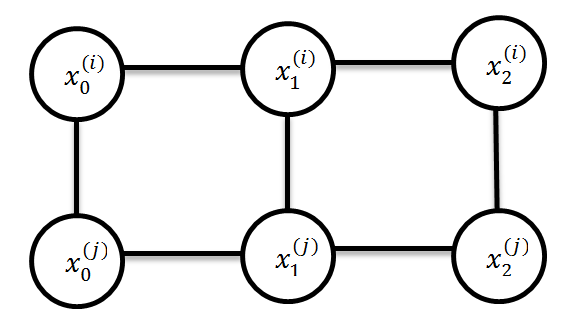
\includegraphics[width=.6\textwidth]{MN.png}
%      \caption{Markov net for cooperative localization of two vehicles. The observation nodes are omitted.}
 %     \label{fig:PMN}
%\end{figure}

%It can be seen that ${\bf \Lambda}_{\bf xz}$ are zeros everywhere but the block diagonals corresponding to each pair of sets $[{x}_{A,i}^\top, {x}_{B,i}^\top]^\top$ and $[{y}_{A,i}^\top, {y}_{B,i}^\top, {y}_{r,i}^\top]^\top$.


%\section{Unwrapped Graphical Model with Information Double Counting}
%\label{sec:unwrapped}

A distributed \textit{na\"ive} filter simply ignores the inter-vehicle correlation and treats the information from the two vehicles as independent. We represent the estimation which ignores the correlation by unwrapping the full graphic model. We show how the \textit{na\"ive} filtering deviates from the central estimator. The unwrapped network has all symbols with a tilde on top, for example, estimated mean is $\tilde\mu$, estimated covariance is $\tilde\sigma^2$, and actual error covariance is $\tilde\delta^2$ of the estimated mean.

\begin{figure}[htbp]
\begin{center}
\subfigure[Full graph (k=1).]{
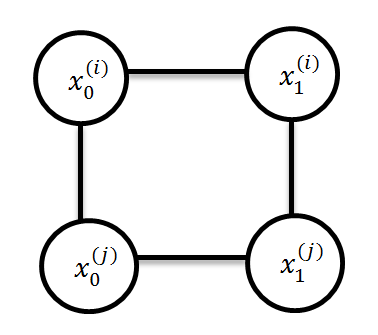
\includegraphics[width=0.45\textwidth]{MNk1}
\label{subfig:PMNk1}
}
\subfigure[Unwrapped graph (k=1).]{
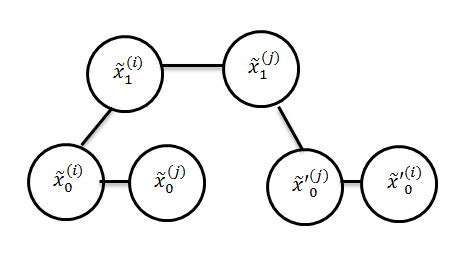
\includegraphics[width=0.45\textwidth]{UNMNk1}
\label{subfig:UNPMNk1}
}
\subfigure[Full graph (k=2).]{
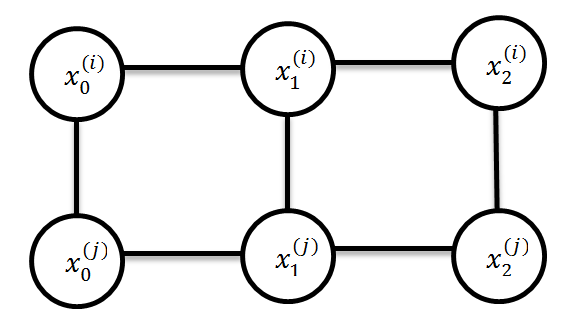
\includegraphics[width=0.65\textwidth]{MN}
\label{subfig:PMNk2}
}
\subfigure[Unwrapped graph (k=2).]{
\includegraphics[width=0.8\textwidth]{UNMNk2}
\label{subfig:UNMNk2}
}
\caption{Full graph vs. Unwrapped graph with information double counting for $k=1,2$: the prime symbol indicates the replication of nodes.}
\label{fig:LOOPYvsUN}
\end{center}
\end{figure}

We plot the unwrapped graphs in Figure~\ref{fig:LOOPYvsUN} for $k=1,2$. It can be seen that the unwrapping simply replicates the past nodes exponentially with ${\bf x}^{(i)}_{k}$ and ${\bf x}^{(j)}_{k}$ being the root nodes. The unwrapped structure assumes the duplicated nodes are from independent sources (independent priors and observations). The exact inference for the unwrapped network is obtained by
\begin{equation}
\label{eq:tildeEI}
\tilde{\bf \Lambda}_{\bf xx}{\bf{\hat{\tilde x}}}=\tilde{\bf P}_{\bf xx}^{-1}\tilde\mu_{\bf x}-\tilde{\bf \Lambda}_{\bf xz}\tilde{\bf z}.
\end{equation}
The replication from the original full network is represented by the mapping matrices ${\bf O}_{\bf x}$ and ${\bf O}_{\bf z}$ such that
\begin{equation}
\begin{split}
{\bf\tilde x}&={\bf O}_{\bf x}{\bf x} \\
{\bf\tilde z}&={\bf O}_{\bf z}{\bf z}. \\
\end{split}
\end{equation}
For example, for $k=1$, the mapping matrices are
\begin{equation}
\begin{split}
{\bf O}_{\bf x}&=\left[
             \begin{array}{cc}
               \bf 1 & \bf 0 \\
               \bf 0 & \bf 1 \\
               \bf 0 & \bf 1 \\
             \end{array}
           \right]=\left[
               \begin{array}{cccc}
                 1 & 0 & 0 & 0 \\
                 0 & 1 & 0 & 0 \\
                 0 & 0 & 1 & 0 \\
                 0 & 0 & 0 & 1 \\
                 0 & 0 & 1 & 0 \\
                 0 & 0 & 0 & 1 \\
               \end{array}
             \right]\\
{\bf O}_{\bf z}&=\left[
             \begin{array}{cc}
               \bf 1 & \bf 0 \\
               \bf 0 & \bf 1 \\
               \bf 0 & \bf 1 \\
             \end{array}
           \right]=\left[
               \begin{array}{cccccc}
                 1 & 0 & 0 & 0 & 0 & 0\\
                 0 & 1 & 0 & 0 & 0 & 0\\
                 0 & 0 & 1 & 0 & 0 & 0\\
                 0 & 0 & 0 & 1 & 0 & 0\\
                 0 & 0 & 0 & 0 & 1 & 0\\
                 0 & 0 & 0 & 0 & 0 & 1\\
                 0 & 0 & 0 & 1 & 0 & 0\\
                 0 & 0 & 0 & 0 & 1 & 0\\
                 0 & 0 & 0 & 0 & 0 & 1\\
               \end{array}
             \right]
\end{split}
\end{equation}
where the bold zeros and ones are the block zero matrix and identity matrix respectively, in appropriate sizes ($2\times 2$ for ${\bf O}_{\bf x}$ and $3\times 3$ for ${\bf O}_{\bf z}$). For $k=2$, we have
\begin{equation}
{\bf O}_{\bf x}=\left[
             \begin{array}{ccc}
               \bf 1 & \bf 0 & \bf 0 \\
               \bf 0 & \bf 1 & \bf 0 \\
               \bf 0 & \bf 0 & \bf 1 \\
                \bf 0 & \bf 1 & \bf 0 \\
               \bf 0 & \bf 0 & \bf 1 \\
               \bf 0 & \bf 0 & \bf 1 \\
               \bf 0 & \bf 0 & \bf 1 \\
             \end{array}
           \right]. \\
\end{equation}

In the mapping, state variables $\tilde{\bf x}_{i}$, $\tilde{\bf x}_{i}'$, $\tilde{\bf x}_{i}''$ and so on are copies of ${\bf x}_{i}$; so are the observations. However, the unwrapped network enables a way for the estimation not to count in the duplication. The independence assumptions are reflected in the structure of $\tilde{\bf \Lambda}$. The precision matrix ($\bf \Lambda$ or $\tilde{\bf \Lambda})$ describes the pairwise statistical relationship given all other nodes. In a Markov network, the entries of precision matrix are only nonzero for neighboring nodes. The relationship between the precision matrices $\bf\tilde \Lambda$ and $\bf \Lambda$ is listed below:
\begin{enumerate}
  \item \underline{${\tilde{\bf \Lambda}}_{\bf xz}{\bf O}_{\bf z}={\bf O}_{\bf x}{\bf \Lambda}_{\bf xz}$ and ${{\bf \Lambda}}_{\bf xz}{\bf O}_{\bf z}^\top={\bf O}_{\bf x}^\top\tilde{\bf \Lambda}_{\bf xz}$:} as ${\bf \Lambda}_{\bf xz}$ is block-diagonal and the block diagonals of $\tilde{\bf \Lambda}_{\bf xz}$ are simply replicates of the block diagonals of ${\bf \Lambda}_{\bf xz}$. ${\bf \Lambda}_{\bf xz}$ and $\tilde{\bf \Lambda}_{\bf xz}$ are equal after partially being projected to each other's domain.
  \item \underline{${\bf \Lambda}_{\bf zz}$ and $\tilde{\bf \Lambda}_{\bf zz}$ are diagonal matrices  and ${\bf O}_{\bf z}{\bf \Lambda}_{\bf zz}^{-1}=\tilde{\bf \Lambda}_{\bf zz}^{-1}{\bf O}_{\bf z}$:} ${\bf \Lambda}_{\bf zz}^{-1}$ is the diagonal observation error covariance matrix. $\tilde{\bf \Lambda}_{\bf zz}^{-1}$ replicates the block diagonals (set of observations) of ${\bf \Lambda}_{\bf zz}^{-1}$. Similarly, ${\bf \Lambda}_{\bf zz}^{-1}$ and $\tilde{\bf \Lambda}_{\bf zz}^{-1}$ are equal after partially being projected to each other's domain.
  \item \underline{An error matrix $\bf E$ is defined such that ${\tilde{\bf \Lambda}}_{\bf xx}{\bf O}_{\bf x}+{\bf E}={\bf O}_{\bf x}{\bf \Lambda}_{\bf xx}$:} the row of $\bf E$ consists all zeros for the nodes who have the same neighbors in the unwrapped network as the original nodes in the full network.
  \item \underline{${\bf E}=-(\tilde{\bf P}_{\bf xx}^{-1}{\bf O}_{\bf x}-{\bf O}_{\bf x}{\bf P}_{\bf xx}^{-1})$:} the property is proved by using block matrix inversion and the relationship summarized above.
\end{enumerate}

\begin{proof}%[Proof of ${\bf E}=-(\tilde{\bf P}_{\bf xx}^{-1}{\bf O}_{\bf x}-{\bf O}_{\bf x}{\bf P}_{\bf xx}^{-1})$]


Using the block matrix inversions
\begin{equation*}
\begin{split}
{\bf P}_{\bf xx}^{-1}&={\bf \Lambda}_{\bf xx}-{\bf \Lambda}_{\bf xz}{\bf \Lambda}_{\bf zz}^{-1}{\bf \Lambda}_{\bf xz}^\top, \\
\tilde{\bf P}_{\bf xx}^{-1}&=\tilde{\bf \Lambda}_{\bf xx}-\tilde{\bf \Lambda}_{\bf xz}\tilde{\bf \Lambda}_{\bf zz}^{-1}\tilde{\bf \Lambda}_{\bf xz}^\top,\\
\end{split}
\end{equation*}
we have
\begin{align*}
%\begin{eqnarray*}
&{\bf O}_{\bf x}({\bf \Lambda}_{\bf xx}-{\bf P}_{\bf xx}^{-1})-(\tilde{\bf \Lambda}_{\bf xx}-\tilde{\bf P}_{\bf xx}^{-1}){\bf O}_{\bf x} & \\
=&{\bf O}_{\bf x}\underline{{\bf \Lambda}_{\bf xz}{\bf \Lambda}_{\bf zz}^{-1}{\bf \Lambda}_{\bf xz}^\top}-\underline{\tilde{\bf \Lambda}_{\bf xz}\tilde{\bf \Lambda}_{\bf zz}^{-1}\tilde{\bf \Lambda}_{\bf xz}^\top}{\bf O}_{\bf x} & \textrm{by block matrix inversion}\\
=&\underline{\tilde{\bf \Lambda}_{\bf xz}{\bf O}_{\bf z}}{\bf \Lambda}_{\bf zz}^{-1}{\bf \Lambda}_{\bf xz}^\top-\tilde{\bf \Lambda}_{\bf xz}\tilde{\bf \Lambda}_{\bf zz}^{-1}\underline{{\bf O}_{\bf z}{\bf \Lambda}_{\bf xz}^\top} & \textrm{by relationship between ${\bf \Lambda}_{\bf xz}$ and $\tilde{\bf \Lambda}_{\bf xz}$}\\
=&\tilde{\bf \Lambda}_{\bf xz}({\bf O}_{\bf z}{\bf \Lambda}_{\bf zz}^{-1}-\tilde{\bf \Lambda}_{\bf zz}^{-1}{\bf O}_{\bf z}){\bf \Lambda}_{\bf xz}^\top & \textrm{grouping the similar terms}\\
%=&\tilde{\bf \Lambda}_{xz}({\bf O}_y{\bf \Lambda}_{xz}^\top-\tilde{\bf \Lambda}_{xz}^\top{\bf O}_{\bf x}) &\\
%=&\tilde{\bf \Lambda}_{xz}({\bf \Lambda}_{xz}{\bf O}_y^\top-{\bf O}_{\bf x}^\top\tilde{\bf \Lambda}_{xz})^\top &\\
=&\bf 0. & \textrm{as ${\bf O}_{\bf z}{\bf \Lambda}_{\bf zz}^{-1}=\tilde{\bf \Lambda}_{\bf zz}^{-1}{\bf O}_{\bf z}$}\\
\end{align*}
%\end{eqnarray*}
The changes in the deviation are underlined, and explanations given on the same lines. Meanwhile, as the error matrix is defined as ${\bf E}={\bf O}_{\bf x}{\bf \Lambda}_{\bf xx}-{\tilde{\bf \Lambda}}_{\bf xx}{\bf O}_{\bf x}$, we have
\begin{equation*}
{\bf O}_{\bf x}({\bf \Lambda}_{\bf xx}-{\bf P}_{\bf xx}^{-1})-(\tilde{\bf \Lambda}_{\bf xx}-\tilde{\bf P}_{\bf xx}^{-1}){\bf O}_{\bf x}={\bf E}+(\tilde{\bf P}_{\bf xx}^{-1}{\bf O}_{\bf x}-{\bf O}_{\bf x}{\bf P}_{\bf xx}^{-1}).\\
\end{equation*}
Therefore
\begin{equation*}
{\bf E}=-(\tilde{\bf P}_{\bf xx}^{-1}{\bf O}_{\bf x}-{\bf O}_{\bf x}{\bf P}_{\bf xx}^{-1}).
\end{equation*}
\end{proof}
The relationship and properties here will be used in the proofs in the following sections.

\subsubsection{Estimated Covariance}

The inference about the estimated covariance of node $\tilde{\bf x}^{(i)}_{k}$ was derived in \cite{Weiss1999} but we restate it as there is some difference in the way of unwrapping.
Let $\bf e$ be a column vector with the first element valued as 1 and all other elements, zero (${\bf e}(1)=1$ and ${\bf e}(i)=0,i\neq 1$).
\begin{align}
%\begin{eqnarray}
{\bf \Lambda}_{\bf xx}{\bf C}_{\bf x|z}&={\bf I} &  \\
{\bf \Lambda}_{\bf xx}{\bf C}_{{\bf x}(1)|{\bf z}}^\top&={\bf e} & \textrm{taking first column of each side} \\
{\bf O}_{\bf x}{\bf \Lambda}_{\bf xx}{\bf C}_{{\bf x}(1)|{\bf z}}^\top&={\bf O}_{\bf x}{\bf e}  & \textrm{left-multiplied by ${\bf O}_{\bf x}$}\\
({\tilde{\bf \Lambda}}_{\bf xx}{\bf O}_{\bf x}+{\bf E}){\bf C}_{{\bf x}(1)|{\bf z}}^\top&={\bf O}_{\bf x}{\bf e}  & \textrm{as ${\tilde{\bf \Lambda}}_{\bf xx}{\bf O}_{\bf x}+{\bf E}={\bf O}_{\bf x}{\bf \Lambda}_{\bf xx}$}\\
{\tilde{\bf \Lambda}}_{\bf xx}{\bf O}_{\bf x}{\bf C}_{{\bf x}(1)|{\bf z}}^\top+{\bf E}{\bf C}_{{\bf x}(1)|{\bf z}}^\top&={\bf O}_{\bf x}{\bf e}.  &\label{eq:fullnetwork}
%\end{eqnarray}
\end{align}
For the unwrapped network, we have similar equation
\begin{equation} \label{eq:unwrappednetwork}
\tilde{\bf \Lambda}_{\bf xx}\tilde{\bf C}_{{\bf x}(1)|y}^\top=\tilde{\bf e}.
\end{equation}
We subtract Equation~\eqref{eq:unwrappednetwork} from Equation~\eqref{eq:fullnetwork} and get
\begin{equation}
\begin{split}
\tilde{\bf \Lambda}_{\bf xx}\tilde{\bf C}_{{\bf x}(1)|{\bf z}}^\top&={\tilde{\bf \Lambda}}_{\bf xx}{\bf O}_{\bf x}{\bf C}_{{\bf x}(1)|{\bf z}}^\top+{\bf E}{\bf C}_{{\bf x}(1)|{\bf z}}^\top+\tilde{\bf e}-{\bf O}_{\bf x}{\bf e} \\
\tilde{\bf C}_{{\bf x}(1)|{\bf z}}^\top&={\bf O}_{\bf x}{\bf C}_{{\bf x}(1)|{\bf z}}^\top+\tilde{\bf \Lambda}_{\bf xx}^{-1}{\bf E}{\bf C}_{{\bf x}(1)|{\bf z}}^\top+\tilde{\bf \Lambda}_{\bf xx}^{-1}(\tilde{\bf e}-{\bf O}_{\bf x}{\bf e}). \\
\end{split}
\end{equation}
As the first row of $\tilde{\bf \Lambda}_{\bf xx}^{-1}$ is $\tilde{\bf C}_{{\bf x}(1)|{\bf z}}$, taking the first element (row) of both sides gives the relationship between $\tilde\sigma^2$ and $\sigma^2$
\begin{equation}
\begin{split}
\label{eq:sigma}
\tilde\sigma^2&=\sigma^2+\tilde{\bf C}_{{\bf x}(1)|{\bf z}}{\bf E}{\bf C}_{{\bf x}(1)|{\bf z}}^\top+\tilde{\bf C}_{{\bf x}(1)|{\bf z}}(\tilde{\bf e}-{\bf O}_{\bf x}{\bf e}) \\
&=\sigma^2+\tilde{\bf C}_{{\bf x}(1)|{\bf z}}{\bf E}{\bf C}_{{\bf x}(1)|{\bf z}}^\top.
\end{split}
\end{equation}
The last term is dropped as our unwrapping contains no duplication of the root node and therefore $\tilde{\bf e}-{\bf O}_{\bf x}{\bf e}=\bf 0$.

The difference $\tilde{\bf C}_{{\bf x}(1)|{\bf z}}{\bf E}{\bf C}_{{\bf x}(1)|{\bf z}}^\top$ in Equation~\eqref{eq:sigma} is actually the first element (entry $(1,1)$) of matrix multiplication $\tilde{\bf C}_{\bf x|z}{\bf E}{\bf C}_{\bf x|z}^\top$. We have
\begin{equation}
\begin{split}
\tilde{\bf C}_{\bf x|z}{\bf E}{\bf C}_{\bf x|z}^\top&=\tilde{\bf \Lambda}_{\bf xx}^{-1}({\bf O}_{\bf x}{\bf \Lambda}_{\bf xx}-\tilde{\bf \Lambda}_{\bf xx}{\bf O}_{\bf x}){\bf \Lambda}_{\bf xx}^{-\top} \\
&=\tilde{\bf \Lambda}_{\bf xx}^{-1}{\bf O}_{\bf x}-{\bf O}_{\bf x}{\bf \Lambda}_{\bf xx}^{-1}. \\
\end{split}
\end{equation}
The first element of these two terms in subtraction are just $\tilde\sigma^2$ and $\sigma^2$.\

%\textbf{How to we prove that $\tilde{\bf C}_{{\bf x}(1)|{\bf z}}{\bf E}{\bf C}_{{\bf x}(1)|{\bf z}}^\top$  is negative?}

\subsubsection{Estimated Mean}
Using the relationship ${\tilde{\bf \Lambda}}_{\bf xz}{\bf O}_{\bf z}={\bf O}_{\bf x}{\bf \Lambda}_{\bf xz}$, Equation~\eqref{eq:tildeEI} is
\begin{equation}
\begin{split}
\tilde{\bf \Lambda}_{\bf xx}{\bf{\hat{\tilde x}}}&=\tilde{\bf P}_{\bf xx}^{-1}\tilde\mu_{\bf x}-\tilde{\bf \Lambda}_{\bf xz}\tilde{\bf z} \\
&=\tilde{\bf P}_{\bf xx}^{-1}{\bf O}_{\bf x}\mu_{\bf x}-\tilde{\bf \Lambda}_{\bf xz}{\bf O}_{\bf z}{\bf z} \\
&=\tilde{\bf P}_{\bf xx}^{-1}{\bf O}_{\bf x}\mu_{\bf x}-{\bf O}_{\bf x}{\bf \Lambda}_{\bf xz}{\bf z}. \\
\end{split}
\end{equation}
We subtract the above equation from a left-multiplied Equation~\eqref{eq:EI} by ${\bf O}_{\bf x}$
\begin{equation}
{\bf O}_{\bf x}{\bf \Lambda}_{\bf xx}{\bf{\hat x}}={\bf O}_{\bf x}{\bf P}_{\bf xx}^{-1}\mu_{\bf x}-{\bf O}_{\bf x}{\bf \Lambda}_{\bf xz}{\bf z}
\end{equation}
and we obtain
\begin{align*}
\tilde{\bf \Lambda}_{\bf xx}{\bf{\hat{\tilde x}}}&={\bf O}_{\bf x}{\bf \Lambda}_{\bf xx}{\bf{\hat{x}}}+\tilde{\bf P}_{\bf xx}^{-1}{\bf O}_{\bf x}\mu_{\bf x}-{\bf O}_{\bf x}{\bf P}_{\bf xx}^{-1}\mu_{\bf x} & \textrm{rearranging the subtraction}\\
&=({\tilde{\bf \Lambda}}_{\bf xx}{\bf O}_{\bf x}+{\bf E}){\bf{\hat{x}}}+(\tilde{\bf P}_{\bf xx}^{-1}{\bf O}_{\bf x}-{\bf O}_{\bf x}{\bf P}_{\bf xx}^{-1})\mu_{\bf x} & \textrm{by grouping similar terms}\\
&={\tilde{\bf \Lambda}}_{\bf xx}{\bf O}_{\bf x}{\bf{\hat{x}}}+{\bf E}{\bf{\hat{x}}}+(\tilde{\bf P}_{\bf xx}^{-1}{\bf O}_{\bf x}-{\bf O}_{\bf x}{\bf P}_{\bf xx}^{-1})\mu_{\bf x} &\\
{\bf{\hat{\tilde x}}}&={\bf O}_{\bf x}{\bf{\hat{x}}}+\tilde{\bf \Lambda}_{\bf xx}^{-1}{\bf E}{\bf{\hat{x}}}+\tilde{\bf \Lambda}_{\bf xx}^{-1}(\tilde{\bf P}_{\bf xx}^{-1}{\bf O}_{\bf x}-{\bf O}_{\bf x}{\bf P}_{\bf xx}^{-1})\mu_{\bf x}. &\\
\end{align*}
Taking the first element (row) of the estimated mean, we have
\begin{equation}
\begin{split}
{\bf{\hat{\tilde x}}}^{(i)}&={\bf{\hat{ x}}}^{(i)}+\tilde{\bf C}_{{\bf x}(1)|{\bf z}}{\bf E}\mu+\tilde{\bf C}_{{\bf x}(1)|{\bf z}}(\tilde{\bf P}_{\bf xx}^{-1}{\bf O}_{\bf x}-{\bf O}_{\bf x}{\bf P}_{\bf xx}^{-1})\mu_{\bf x} \\
&={\bf{\hat{ x}}}^{(i)}+\tilde{\bf C}_{{\bf x}(1)|{\bf z}}{\bf E}{\bf{\hat{x}}}-\tilde{\bf C}_{{\bf x}(1)|{\bf z}}{\bf E}\mu_{\bf x} \\
&={\bf{\hat{ x}}}^{(i)}+\tilde{\bf C}_{{\bf x}(1)|{\bf z}}{\bf E}({\bf{\hat{x}}}-\mu_{\bf x}). \\
\end{split}
\end{equation}

We now analyze the the performance of the estimated mean which includes:
\begin{itemize}
  \item The mean error of the estimated mean $\mathbb{E}[{\bf{\hat{\tilde x}}}^{(i)}-{\bf x}^{(i)}_{k}]$, and
  \item The error covariance of the estimated mean $\tilde\delta^2=\mathbb{E}[({\bf{\hat{\tilde x}}}^{(i)}-{\bf x}^{(i)}_{k})^2]$.
\end{itemize}

The mean error of the estimated mean is zero because
\begin{equation}
\begin{split}
\mathbb{E}[{\bf{\hat{\tilde x}}}^{(i)}-{\bf x}^{(i)}_{k}]&=\mathbb{E}[{\bf{\hat{x}}}^{(i)}+\tilde{\bf C}_{{\bf x}(1)|{\bf z}}{\bf E}{\bf{\hat{x}}}-\tilde{\bf C}_{{\bf x}(1)|{\bf z}}{\bf E}\mu_{\bf x}-{\bf x}^{(i)}_{k}] \\
&=\mathbb{E}[{\bf{\hat{x}}}^{(i)}-{\bf x}^{(i)}_{k}]+\tilde{\bf C}_{{\bf x}(1)|{\bf z}}{\bf E}\mathbb{E}[{\bf{\hat{x}}}-\mu_{\bf x}] \\
&=0.
\end{split}
\end{equation}
The two expectations are zero because the estimation error of the original full network is zero-mean. The error covariance of the estimated mean is
\begin{equation}
\begin{split}
\tilde\delta^2&=\mathbb{E}[({\bf{\hat{\tilde x}}}^{(i)}-{\bf x}^{(i)}_{k})^2] \\
&=\mathbb{E}[({\bf{\hat{ x}}}^{(i)}+\tilde{\bf C}_{{\bf x}(1)|{\bf z}}{\bf E}{\bf{\hat{x}}}-\tilde{\bf C}_{{\bf x}(1)|{\bf z}}{\bf E}\mu_{\bf x}-{\bf x}^{(i)}_{k})^2] \\
&=\mathbb{E}[({\bf{\hat{ x}}}^{(i)}-{\bf x}^{(i)}_{k})^2]+\mathbb{E}[(\tilde{\bf C}_{{\bf x}(1)|{\bf z}}{\bf E}({\bf{\hat{x}}}-\mu_{\bf x}))^2]+2\mathbb{E}[({\bf{\hat{ x}}}^{(i)}-{\bf x}^{(i)}_{k})\tilde{\bf C}_{{\bf x}(1)|{\bf z}}{\bf E}({\bf{\hat{x}}}-\mu_{\bf x})]. \\
\end{split}
\end{equation}
In the above equation, the first term $\mathbb{E}[(\mu-x_{A,k})^2]=\sigma^2$, the last term is zero. % (\textbf{need to prove, I believe so and am working on it}).
%\begin{equation}
%\begin{split}
%&\mathbb{E}[(\mu-x_{A,k})\tilde{\bf C}_{{\bf x}(1)|{\bf z}}{\bf E}({\bf{\hat{x}}}-\mu_{\bf x})]\\
%=& \ldots\\
%=&0
%\end{split}
%\end{equation}
The second term
\begin{equation}
\begin{split}
\mathbb{E}[(\tilde{\bf C}_{{\bf x}(1)|{\bf z}}{\bf E}({\bf{\hat{x}}}-\mu_{\bf x}))^2]
&=\mathbb{E}[\tilde{\bf C}_{{\bf x}(1)|{\bf z}}{\bf E}({\bf{\hat{x}}}-\mu_{\bf x})({\bf{\hat{x}}}-\mu_{\bf x})^\top{\bf E}^\top\tilde{\bf C}_{{\bf x}(1)|{\bf z}}^\top] \\
&=\tilde{\bf C}_{{\bf x}(1)|{\bf z}}{\bf E}\mathbb{E}[({\bf{\hat{x}}}-\mu_{\bf x})({\bf{\hat{x}}}-\mu_{\bf x})^\top]{\bf E}^\top\tilde{\bf C}_{{\bf x}(1)|{\bf z}}^\top \\
&=\tilde{\bf C}_{{\bf x}(1)|{\bf z}}{\bf E}({\bf P}_{\bf xx}-{\bf \Lambda}_{\bf xx}^{-1}){\bf E}^\top\tilde{\bf C}_{{\bf x}(1)|{\bf z}}^\top. \\
\end{split}
\end{equation}
Therefore, the error covariance of the estimated mean is
\begin{equation}
\begin{split}
\tilde\delta^2&=\sigma^2+\tilde{\bf C}_{{\bf x}(1)|{\bf z}}{\bf E}({\bf P}_{\bf xx}-{\bf \Lambda}_{\bf xx}^{-1}){\bf E}^\top\tilde{\bf C}_{{\bf x}(1)|{\bf z}}^\top \\
&=\delta^2+\tilde{\bf C}_{{\bf x}(1)|{\bf z}}{\bf E}({\bf P}_{\bf xx}-{\bf \Lambda}_{\bf xx}^{-1}){\bf E}^\top\tilde{\bf C}_{{\bf x}(1)|{\bf z}}^\top.
\end{split}
\end{equation}
It is easy to see that ${\bf P}_{\bf xx}\succeq{\bf \Lambda}_{\bf xx}^{-1}$ and $\tilde{\bf C}_{{\bf x}(1)|{\bf z}}{\bf E}({\bf P}_{\bf xx}-{\bf \Lambda}_{\bf xx}^{-1}){\bf E}^\top\tilde{\bf C}_{{\bf x}(1)|{\bf z}}^\top\geq 0$. We have $\tilde\delta^2\geq\delta^2=\sigma^2$.
\subsubsection{Summary of the Relationship}
%$$\boxed{u=1}$$
%$$
\begin{equation}
\boxed{
\begin{aligned}
\tilde\sigma^2&=\sigma^2+\tilde{\bf C}_{{\bf x}(1)|{\bf z}}{\bf E}{\bf C}_{{\bf x}(1)|{\bf z}}^\top \\
{\bf{\hat{\tilde x}}}^{(i)}&={\bf{\hat{ x}}}^{(i)}+\tilde{\bf C}_{{\bf x}(1)|{\bf z}}{\bf E}({\bf \hat x}-\mu_{\bf x})\\
\mathbb{E}[{\bf{\hat{\tilde x}}}^{(i)}-{\bf x}^{(i)}_{k}]&=0 \\
\mathbb{E}[({\bf{\hat{\tilde x}}}^{(i)}-{\bf x}^{(i)}_{k})^2]&=\tilde\delta^2=\delta^2+\tilde{\bf C}_{{\bf x}(1)|{\bf z}}{\bf E}({\bf P}_{\bf xx}-{\bf \Lambda}_{\bf xx}^{-1}){\bf E}^\top\tilde{\bf C}_{{\bf x}(1)|{\bf z}}^\top
\end{aligned}
} \\
\end{equation}
%We should be able to show the relationship (\textbf{Need to prove $\tilde\sigma^2\leq\sigma^2$})
%\begin{equation}
%\tilde\sigma^2\leq\sigma^2=\delta^2\leq\tilde\delta^2
%\end{equation}
By constructing the unwrapped network of \textit{na\"ive} filter, we derive the performance of the \textit{na\"ive} filter compared with central filter using the summarized equations above. The estimation overconfidence can be explained by the first relationship. The estimation divergence comes from the second and fourth equations but it is not easy to visualize. We shall quantify the divergence region in the next section.

% We are interested to know the limiting stable performance of the error covariance of the estimate, when $k=+\infty$. Firstly, we look at the limiting difference of the error covariance of the estimate with respect to the optimal error covariance given in the central architecture:
% \begin{equation}
% \begin{split}
% \tilde\delta^2-\sigma^2&=\tilde{\bf C}_{{\bf x}(1)|{\bf z}}{\bf E}({\bf P}_{\bf xx}-{\bf \Lambda}_{\bf xx}^{-1}){\bf E}^\top\tilde{\bf C}_{{\bf x}(1)|{\bf z}}^\top \\
% &\leq\tilde{\bf C}_{{\bf x}(1)|{\bf z}}{\bf E}{\bf P}_{\bf xx}{\bf E}^\top\tilde{\bf C}_{{\bf x}(1)|{\bf z}}^\top
% \end{split}
% \end{equation}
% We can also look at the difference normalized by $\sigma^2$, that is, $\frac{\tilde\delta^2-\sigma^2}{\sigma^2}$. These term are supposed to be bounded as $\tilde{\bf C}_{{\bf x}(1)|{\bf z}}$ is getting smaller with respect to the nodes further and further way from the root nodes. If we look at the unwrapped structure from $k$ to $k+1$ (Figure~\ref{fig:k3}), it is simply adding nodes to the existing leaf nodes. With the same settings (same values of prior and observation noise distribution), the node adding does not affect the limiting performance of the estimation. %\textbf{How to prove this?}
% \begin{figure}[H]
%   \centering
%     \includegraphics[width=\textwidth]{k3.jpg}      \caption{Unwrapped network extending from $k$ to $k+1$. It is equivalent to adding nodes to the existing leaf nodes. We can see structure for $k=1$ step above the orange dashed line, and structure for $k=2$ steps above the blue dotted line. The green nodes are the ones having different neighboring statistical relationship compared with the original nodes in the full graph.}
%       \label{fig:k3}
% \end{figure}
% Figure~\ref{fig:matrices} color-plots the precision matrices from both structures and the error matrices for $k=1$ and $k=2$.
% \begin{figure}[H]
% \begin{center}
% \subfigure[]{
% 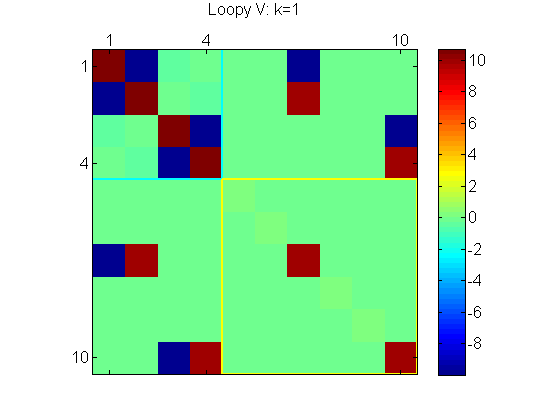
\includegraphics[width=0.45\textwidth]{K1-1.fig}
% \label{subfig:k1-1}
% }
% \subfigure[]{
% 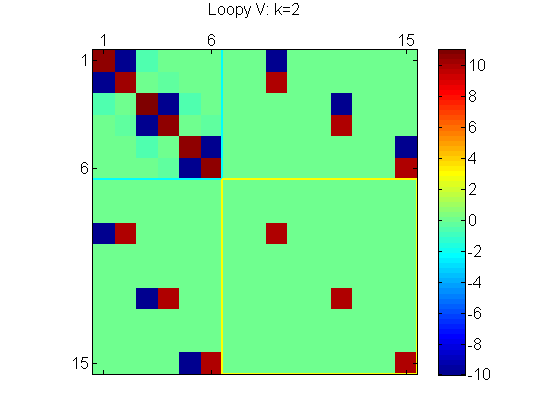
\includegraphics[width=0.45\textwidth]{K2-1}
% \label{subfig:k2-1}
% }
% \subfigure[]{
% 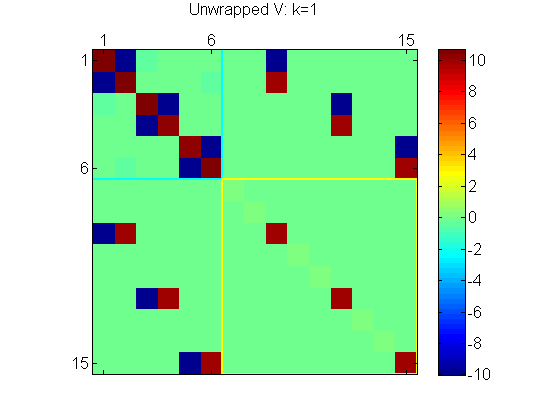
\includegraphics[width=0.45\textwidth]{K1-2}
% \label{subfig:k1-2}
% }
% \subfigure[]{
% 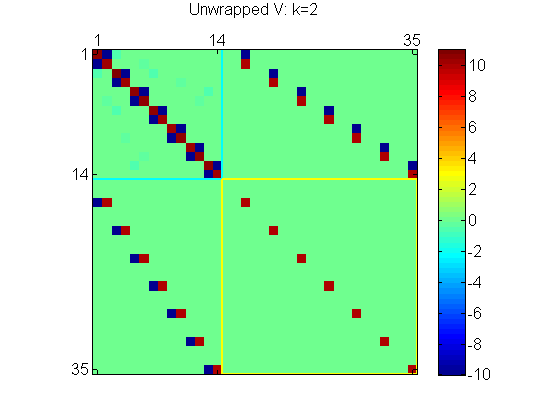
\includegraphics[width=0.45\textwidth]{K2-2}
% \label{subfig:k2-2}
% }
% \subfigure[]{
% 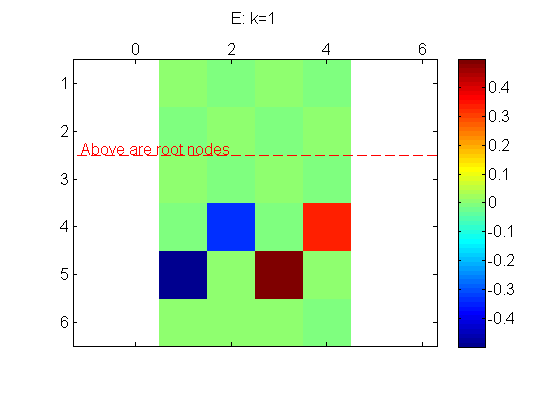
\includegraphics[width=0.45\textwidth]{K1-3}
% \label{subfig:k1-3}
% }
% \subfigure[]{
% 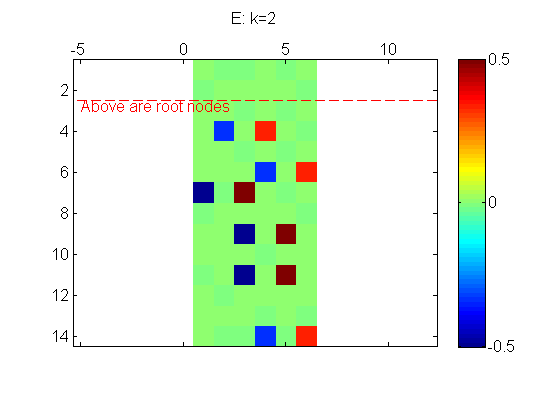
\includegraphics[width=0.45\textwidth]{K2-3-}
% \label{subfig:k2-3}
% }
% \caption{Precision matrices and error matrices for $k=1$ (left column) and $k=2$ (right column).}
% \label{fig:matrices}
% \end{center}
% \end{figure}


% If we rearrange the node sequence in the unwrapped state vector for $k=2$ such that $\tilde{\bf x}=[\tilde{x}_{A,2}^\top, \tilde{x}_{B,2}^\top,\tilde{x}_{A,1}^\top, \tilde{x}_{B,1}^\top,\tilde{x'}_{A,1}^\top, \tilde{x'}_{B,1}^\top,\tilde{x}_{A,0}^\top, \tilde{x}_{B,0}^\top, \tilde{x'}_{A,0}^\top, \tilde{x'}_{B,0}^\top, \tilde{x''}_{A,0}^\top, \tilde{x''}_{B,0}^\top, \tilde{x'''}_{A,0}^\top, \tilde{x'''}_{B,0}^\top]^\top$ (we rearrange the sequence of $y$ accordingly), we can see in Figure~\ref{fig:matrices-re} that the error matrix $\bf E$ is simply adding rows of difference to the $\bf E$ for $k=1$. In this case, the mapping matrix ${\bf O}_{\bf x}=\left[
%              \begin{array}{ccc}
%               \bf 1 & \bf 0 & \bf 0 \\
%               \bf 0 & \bf 1 & \bf 0 \\
%               \bf 0 & \bf 1 & \bf 0 \\
%                 \bf 0 & \bf 0 & \bf 1 \\
%               \bf 0 & \bf 0 & \bf 1 \\
%               \bf 0 & \bf 0 & \bf 1 \\
%               \bf 0 & \bf 0 & \bf 1 \\
%              \end{array}
%           \right]
% $.
% \begin{figure}[H]
% \begin{center}
% \subfigure[]{
% 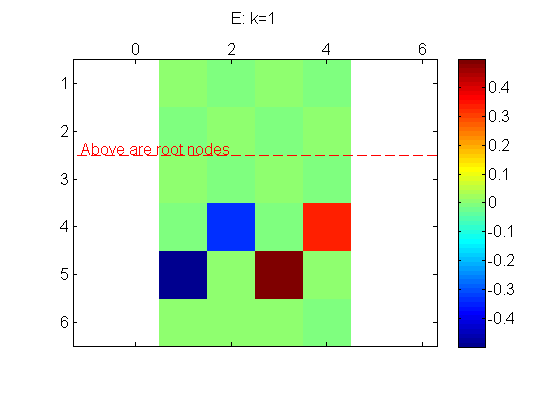
\includegraphics[width=0.45\textwidth]{K1-3}
% \label{subfig:k1-3}
% }
% \subfigure[]{
% 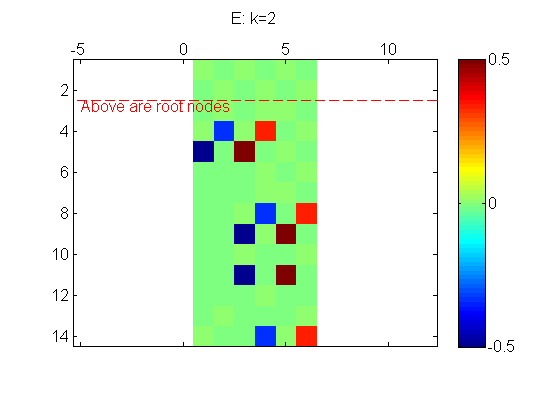
\includegraphics[width=0.45\textwidth]{K2-3}
% \label{subfig:k2-3}
% }
% \caption{Error matrices for $k=1$ (left column) and $k=2$ with rearranged states (right column).}
% \label{fig:matrices-re}
% \end{center}
% \end{figure}
% If you read Yair Weiss paper, there is a difference in unwrapping the original problem. In his paper, the original full network is unwrapped in a way that all non-leaf nodes in the unwrapped structure maintain the same neighboring statistical relationship. We do not have that in our DKF estimation. We assume that all the duplicated nodes for relative measurement updates have no statistical relationship with the future nodes.

% A naive extended Kalman filter (NEKF) does not track the correlation among vehicles; they are always assumed to be independent to one another. This results in a double-counting of information as one vehicle's state may have been used previously. Inconsistent estimate appears where vehicles are overconfident about its own positioning. In this case, less information will be gained from some accurate and important measurements.
% Suboptimal estimation with unknown correlation

% example of information double counting in paper.

% \begin{itemize}

%   \item information flow in partially connected network
% \item Turbo decoder etc for iterative decoding algorithm

% \end{itemize}

\subsection{Multi-Vehicle Localization with Bathymetric Aids}

The multi-vehicle localization consists of vehicles estimating their own positions, and cooperating with an additional relative measurement relating the two vehicles. When bathymetry map is used to assist the localization, the local measurements consist of water depth measurements, and they are fairly accurate. We look at conditions under which correlation can be ignored.

We consider the recursive two-step process where two vehicles (Vehicle $i=1$ and $j=2$) localize themselves (position states ${\bf x}^{(1)}$ and ${\bf x}^{(2)}$) respectively. Similarly we denote previous time step $k$ and current time step $k+1$. At each step, each node makes a local observation (${\bf z}^{(1)}$ or ${\bf z}^{(2)}$) about their respective positions. A range measurement ${\bf r}$ is made between vehicles. The propagation model in Equation~\eqref{eq:mvlpropagation} is simplified as a random walk process
\begin{equation}
\begin{split}
{\bf x}_{k+1}^{(1)}&={\bf x}_k^{(1)}+{\bf \omega}_k^{(1)}\\
{\bf x}_{k+1}^{(2)}&={\bf x}_k^{(2)}+{\bf \omega}_k^{(2)}.\\
\end{split}
\end{equation}
The propagation noises are independent of each other with the same error covariance ${\bf Q}$. The measurements ${\bf z}_k^{(1)}$, ${\bf z}_k^{(2)}$ and $r_k$ in Equation~\eqref{eq:mvlmeasurement} have error covariance ${\bf R}^{(1)}$, ${\bf R}^{(2)}$ and ${\bf R}_r$ respectively. Without loss of generality, we assume ${\bf R}^{(1)}\leq{\bf R}^{(2)}$.
%and at each step we have
%\begin{equation}
 %   \begin{split}
  %      {\bf z}_1&={\bf x}_1+{\bf \nu}_1 \\
%{\bf z}_2&={\bf x}_2+{\bf \nu}_2\\
%r&={\bf x}_1-{\bf x}_2+\upsilon\\
%\end{split}
%\end{equation}
%where the propagation noise $\bf \omega$ and observation noises ${\bf \nu}_1$, ${\bf \nu}_2$ and $\bf\upsilon$ are independent zero-mean Gaussian processes with covariances ${\bf Q}$, ${\bf R}^{(1)}$, ${\bf R}^{(2)}$ and $\bf R$. Without loss of generality, we assume ${\bf R}^{(1)}\leq{\bf R}^{(2)}$. 

Compared with multi-sensor tracking problem, there are two differences. The first difference lies in an additional variable called ranging $r$ at each step. It relates the two position variables. The second difference comes from individual process noise on position of each vehicle. $\omega_1$ and $\omega_2$ are independent noises.% Large propagation noises increase the inter-vehicle independence.

In step $k$, the estimates at Vehicle $i$ and $j$ are ${\bf y}_k^{(1)}$ and ${\bf y}_k^{(2)}$, with the same error covariance ${\bf P}_k$ and correlation coefficient $\rho_k$. Central KF stacks the two state variables and the centralized error covariance is therefore 
%\begin{equation}
 %   \begin{split}
 %       {\bf\bar y}_1&={\bf\bar x}_1+\bar\varepsilon_1 \\
   %     {\bf\bar y}_2&={\bf\bar x}_2+\bar\varepsilon_2.
  %  \end{split}
%\end{equation}
%The estimation error $\bar\varepsilon_1$ and $\bar\varepsilon_2$ are assumed to have covariance ${\bf\bar P}$ and correlation coefficient $\bar\rho$. The central KF stacks the state variables with error covariance in the previous step as 
$\left[
          \begin{array}{cc}
            {\bf P}_k & \rho_k{\bf P}_k \\
            \rho_k{\bf P}_k & {\bf P}_k\\
          \end{array}
        \right]$. Figure~\ref{fig:CKFeg1} and Figure~\ref{fig:CKFeg2} show two examples of centralized processing, with respect to different values of $\rho_k$ and ${\bf R}_r$. The different settings of the two cases have a common extreme situation: when the ranging error is 0, the two estimates are fully correlated (and therefore have the same error covariance) after cooperation. When the ranging error approaches zero, the two estimates are almost fully correlated with similar error covariance after cooperation.
        
         \begin{figure}[htbp]
\begin{center}
\subfigure[Case 1: Correlation coefficient in one-step cooperation.]{
\includegraphics[width=.8\textwidth]{Figures/CKFrhoVSr.pdf}
\label{subfig:CKFrho}
}
\subfigure[Case 1: Error covariances of two vehicles in one-step cooperation.]{
\includegraphics[width=.8\textwidth]{Figures/CKFp.pdf}
\label{subfig:CKFp}
}
\caption{Case 1: ${\bf P}_k=5,{\bf Q}=10,{\bf R}^{(1)}=1,{\bf R}^{(2)}=2$. When ranging error approaches 0, the two estimates are about fully correlated with similar error covariances after cooperation.}
\label{fig:CKFeg1}
\end{center}
\end{figure}

\begin{figure}[htbp]
\centering
\subfigure[Case 2: Correlation coefficient in one-step cooperation.]{
\includegraphics[width=.8\textwidth]{Figures/CKFrhoVSr2.pdf}
\label{subfig:CKFrho2}
}
\subfigure[Case 2: Error covariances of two vehicles in one-step cooperation.]{
\includegraphics[width=.8\textwidth]{Figures/CKFp2.pdf}
\label{subfig:CKFp2}
}
\caption{Case 2:${\bf P}_k=5,{\bf Q}=1,{\bf R}^{(1)}=10,{\bf R}^{(2)}=40$. When ranging error approaches 0, the two estimates are about fully correlated with similar error covariances after cooperation.}
\label{fig:CKFeg2}
\end{figure}

We also analyze the performance of SF, NF and DF (with a weighting factor). A SF at Vehicle 1 has
\begin{equation}
\begin{split}
    {\bf y}^{(1)}_{k+1}&={\bf y}_k^{(k)}+({\bf P}_k+{\bf Q}^{(1)})({\bf P}_k+{\bf Q}^{(1)}+{\bf R}^{(1)})^{-1}({\bf z}^{(1)}_{k+1}-{\bf y}^{(1)}_{k+1}) \\
    {\bf P}^{(1)}_{k+1}&=({{\bf P}_k}^{-1}+{{\bf R}^{(1)}}^{-1})^{-1}. \\
\end{split}
\end{equation}
This is standard KF and Vehicle 2 obtains its estimation in the same way. NF fuses the estimated position from Vehicle 2 about Vehicle 1 such that ${\bf y}^{(1)}_{\text{NF}}=\lambda_\text{NF}{\bf y}^{(1)}_{k+1}+(1-\lambda_\text{NF})({\bf y}^{(2)}_{k+1}+{r}_{k+1})$, where the weight $\lambda_\text{NF}=({\bf P}^{(2)}_{k+1}+{\bf R}_r)({\bf P}^{(1)}_{k+1}+{\bf P}^{(2)}_{k+1}+{\bf R}_r)^{-1}$.

DF fuses the estimated position from Vehicle 2 using a weight $\lambda_1$ such that ${\bf y}^{(1)}_{\text{DF}}=(1-\lambda_1){\bf y}^{(1)}_{k+1}+\lambda_1({\bf y}^{(2)}_{k+1}+r_{k+1})$. At Vehicle 2, the DF fuses the estimated position from Vehicle 1 using a weight $\lambda_2$ such that ${\bf y}^{(2)}_{\text{DF}}=(1-\lambda_2){\bf y}^{(2)}_{k+1}+\lambda_2({\bf y}^{(1)}_{k+1}-{r}_{k+1})$. The error covariances can be calculated accordingly. The optimal weights can be obtained such that
\begin{equation}
\begin{split}
    \lambda_1^*&=\arg\min\mathbb{E}[({\bf y}^{(1)}_{\text{DF}}-{\bf x}^{(1)}_{k+1})^2]\\
    \lambda_2^*&=\arg\min\mathbb{E}[({\bf y}^{(2)}_{\text{DF}}-{\bf x}^{(2)}_{k+1})^2].\\
\end{split}
\label{eq:mvlDF}
\end{equation}
When ranging error ${\bf R}_r=0$, we have $\lambda_1^*+\lambda_2^*=1$ and the two estimates are fully correlated after cooperation. When the ranging error ${\bf R}_r$ is very small, $\lambda_1^*+\lambda_2^*$ also approaches 1. In underwater communications, we do have the ability to achieve very small ranging error, compared with positioning error. For simplicity, we set ${\bf R}_r=0$ and therefore the correlation coefficient goes to 1.

\subsubsection{One-Step Performance}

We calculate the one-step \textit{dangerous} region, similar to the situation in Equation~\eqref{eq:nffail}, that is
\begin{equation}
 \det\mathbb{E}[({\bf y}^{(1)}_{\text{NF}}-{\bf x}_{k+1})({\bf y}^{(f)}_{\text{NF}}-{\bf x}_{k+1})^\top]>\det{\bf P}_{k+1}^{(1)}.  
 \label{eq:mvlnffail}
\end{equation}

Firstly, we consider the extreme cases. When ${\bf Q}\rightarrow 0$, the inequality is the same as Equation~\eqref{eq:danger} except that the normalized ${\bf\bar R}^{(i)}=\frac{{\bf R}^{(i)}}{{\bf P}_k}$. It has the same region in the two-sensor tracking problem. This is easy to understand as the zero propagation noise makes the two states fully correlated. In such a case, we can see that the DF has the optimal weight $\lambda^*_\text{DF}=\frac{{\bf R}^{(1)}}{{\bf R}^{(1)}+{\bf R}^{(2)}}$. The same result can be derived by minimizing the error covariance in Equation~\eqref{eq:mvlDF}.

When ${\bf Q}\gg{\bf P}_k$ and ${\bf R}^{(i)}\ll{\bf Q}$, NF approaches the performance of CF, because the assumption of independence is almost valid. We can ignore the correlation.

When the propagation noise is neither too small nor too large, we derive the \textit{dangerous} region shown in Figure~\ref{fig:mvlOneStepRegion} when Equation~\eqref{eq:mvlnffail} is met. This region tells us when the local propagation error is small, the states are more correlated. Vehicle 2 maintains most of the correlated information when ${\bf R}^{(2)}>{\bf R}^{(1)}$. In such a case, if the correlation in the estimate from Vehicle 2 is ignored, the fused estimate is worse than the estimate from SF.

\begin{figure}[htbp]
  \centering
    \includegraphics[width=.8\textwidth]{Figures/mvlOneStepRegion.pdf}
      \caption{One-step Performance: The \textit{dangerous} region of implementing NF in multi-vehicle localization. (${\bf\bar R}^{(2)}>{\bf\bar R}^{(1)}$)}
      \label{fig:mvlOneStepRegion}
\end{figure}


\subsubsection{Asymptotic Performance}

Figure~\ref{fig:sscases} shows the estimation performance in stable state. The cases are located in Figure~\ref{fig:mvlssRegion} using their parameter values. The normalized ${\bf\bar R}^{(i)}={\bf R}^{(i)}/{\bf Q}$. In the three cases, cooperative localization with bathymetric aids is most similar to Case (b) and Case (c). The relative distance measured by acoustic signals has small error (${\bf R}_r$ is in the sub-meters range); the local measurement, i.e., the water depth has much smaller errors compared with the propagation errors accumulated between cooperation. Even if any one of the cooperative vehicles has little or none of the bathymetry aids (large measurement error like Case (c)), it is still safe to ignore the correlation.

\begin{figure}[htbp]
\centering
\subfigure[Actual error covariance eventually grows larger than SF.]{
\includegraphics[width=.6\textwidth]{Figures/sscasea.png}
\label{subfig:sscasea}
}
\subfigure[It is safe to ignore correlation and the performance is close to CF.]{
\includegraphics[width=.6\textwidth]{Figures/sscaseb.png}
\label{subfig:sscaseb}
}
\subfigure[Actual error covariance is smaller than SF but the estimation is overconfident.]{
\includegraphics[width=.6\textwidth]{Figures/sscasec.png}
\label{subfig:sscasec}
}
\caption{\textit{Na\"ive} filter in stable state: One can ignore the correlation in Case (b) and Case (c) but NF becomes detrimental in Case (a).}
\label{fig:sscases}
\end{figure}

\begin{figure}[htbp]
  \centering
    \includegraphics[width=.8\textwidth]{Figures/mvlssregion.pdf}
      \caption{Asymptotic Performance: The \textit{dangerous} region of implementing NF in multi-vehicle localization. The three cases in Figure~\ref{fig:sscases}are located in the regions.}
      \label{fig:mvlssRegion}
\end{figure}

\section{Summary}

We demonstrated why there is information loss in distributed localization, and how the information is double counted if one ignores the correlation.

For a cooperation method, when the actual localization is worse than single-vehicle localization, we call it \textit{dangerous} as this cooperation makes the estimation worse. When the actual localization is better than single-vehicle localization, we perceive it safe as this cooperation helps. For both types of cooperative localization - multi-sensor tracking problem and multi-vehicle localization problem, we quantified the safe and \textit{dangerous} regions when ignoring correlation during fusion. This can be used as a guideline to justify the \textit{na\"ive} assumption. The \textit{na\"ive} assumption is justified safe to use in cooperative localization with bathymetric aids in the next chapter.
\chapter{Localization with Bathymetric Aids}
\label{ch:bathymetry}
\lhead{Chapter~\ref{ch:bathymetry}. \emph{Localization with Bathymetric Aids}}


\section{Problem Statement}

Chapter~\ref{ch:naive} shows that cooperative localization with bathymetric aids can ignore the correlation when fusing information from range updates. With this justification, we proceed to explore the bathymetry-aided navigation on a single vehicle. This can be safely extended to cooperative navigation of multiple vehicles. The first work investigates how the bathymetric terrain map benefits the localization. As many works have claimed that the localization performance highly depends on the bathymetry variation \cite{Kalyan2013,Peng2016,Rodrigo2015,Galceran2013}, we justify this assumption through a careful analysis. It is again proved that the advantage of bathymetric aids is path dependent. However the bathymetry variation is not a sufficient condition for a good localization. A concept of information entropy map, is formulated and used in Chapter~\ref{ch:ban} later as an evaluation metric in path planning.

The work in this chapter and Chapter~\ref{ch:ban} was published in~\cite{Gao2018}.

\section{Probability Map Based Localization}

We denote the entire location space at time $k$ as ${\bf{X}}_k$. $\text{Bel}({\bf{X}}_k=x)$ denotes the vehicle's belief that it is at the location $x$ at time $k$. The action ${\bf{a}}_k$ denotes the action taken at time step $k$ towards the next step $k+1$, and ${\bf{A}}_{1:k}\doteq\{{\bf{a}}_1,{\bf{a}}_2,...,{\bf{a}}_k\}$. The same definition and notation apply
to the sensing data ${\bf{y}}_k$. Markov process assumes that given the present state, the future and past states are independent. In formal terms, it is stated
\begin{equation}
{P}({\bf x}_k|{\bf x}_0,...,{\bf x}_{k-1},{\bf a}_0,...,{\bf a}_{k-1},{\bf zS}_0,...,{\bf z}_{k},)={P}({\bf x}_k|{\bf x}_{k-1},{\bf a}_{k-1}).
\end{equation}
This only works if the environment is static and does not change with time \cite{Thrun2005}. Kalman filter described in the previous chapter is one of the common methods used. However, Kalman filter assumes Gaussian noises in estimation and measurements. It does not perform well for situations where the models are nonlinear or the belief is multimodal. For example, a vehicle moving along the ridge of a hill may arrive at a belief that has two peaks at its two sides. In such situations, filters with non-parametric representation can give better description.

Two types of localization methods are introduced in the subsequent sections - grid-based Markove localization and particle filtering. We examine the effect of bathymetry aids on localization. This includes how the bathymetry affects the localization belief, which estimation filter should be used, and how the localization performance should be quantified. %Two types of non-parametric localization are investigated in this section: grid-based Markov localization and Monte Carlo localization.

\subsection{Grid-Based Markov Localization}

% source code: C:\Users\tmsgr\Dropbox\Gao Rui JL_GR\PhD progress\BAN2\St.John - main_Markov.m
The grid-based localization uses a histogram to represent the belief distribution in map grids. We use the algorithm in \cite{dieter1999} to simulate the grid-based Markov localization near St John's Island, Singapore. We assume that we have no idea where the vehicle is at the beginning, and hence we initialize a uniform prior distribution in this area. The grid-based Markov localization has the ability to represent situations where the position of the vehicle is held by multiple, distinct beliefs. The probability could be any form instead of single Gaussian. It also caters to the situation where the initial position is unknown.

There are two steps in the Markov localization: action (propagation) and sensing (observation). The corresponding estimation is to predict and update the belief. The uncertainty in the prediction smooths out the location possibility while the observation for update reinforces the places which have similar water depth (bathymetry) as measured. The resolution of the surveyed bathymetry restricts the accuracy of positioning. The computation load is comparable to the grid map resolution and is fairly high. In the St John's map, for example, we have an area of 936 meters by 349 meters, with 1 meter resolution, giving a total of $326664$ grids, of which $192956$ grids are underwater.

\begin{figure}[htbp]
\centering
%\begin{sideways}
    \includegraphics{./Figures/Bathy_path.png}
     % \end{sideways}
            \caption{Bathymetry map near St. John Island, Singapore. Circles: Path 1 (Speed 2 m/s). Crosses: Path 2 (Speed 1.41m/s).}
                        \label{fig:Bathy_path}
\end{figure}

\begin{figure}[htbp]
\centering
\subfigure[Path 1.]{
\includegraphics[width=\textwidth]{./Figures/all.png}
\label{subfig:path1}
}
\subfigure[Path 2.]{
\includegraphics[width=\textwidth]{./Figures/all2.png}
\label{subfig:path2}
}
\caption{Grid-based Markov localization with measurement updates. Yellow crosses: top 5 possible locations. Cyan circles: true path. Green square: estimated locations with top possibility.}
            %\end{sideways}
              \label{fig:all}
\end{figure}

\begin{figure}[htbp]
\begin{center}
\subfigure[Path 1.]{
\includegraphics[width=0.45\textwidth]{./Figures/depth1.png}
\label{subfig:depth1}
}
\subfigure[Path 2.]{
\includegraphics[width=0.45\textwidth]{./Figures/depth2.png}
\label{subfig:depth2}
}
\caption{Depth measurements along two paths.}
            %\end{sideways}
              \label{fig:depth}
\end{center}
\end{figure}

Figure~\ref{fig:Bathy_path} shows two test paths on the bathymetry map. The simulation assumes of odometric error of 1 meter per second in standard deviation, and measurement error of 0.1 meters in standard deviation. There is a measurement every other 15 seconds. Both start with uniform beliefs on the vehicle location over the map. The decision of the position by the top beliefs at initial few measurements is mostly incorrect as there could be many locations with similar top probability. Multiple hypotheses on the location appears. With more bathymetry measurements (from left to right in Figure~\ref{fig:all}), the probability is updated from multiple peaks or ridges to eventually a single peak. The decision on the estimated position converges. However Path 2 localization converges from the second depth measurement onward, whereas Path 1 localization only converges at the 4th measurement. In terms of bathymetry variations along the path, Path 1 has more variations as shown in Figure~\ref{fig:depth}. The underwater topology variations (richness of features) on the path are closely related to the positioning performance. The sparser the underwater topology, the less effective are bathymetry aids to localization. However bathymetry variation is not the sufficient or necessary condition for a good localization. The uniqueness of the measured depth compared with the bathymetry in the prior belief decides the localization performance. Multiple AUVs with cooperation are able to extract more uniqueness in the feature space.

\subsection{Particle Filtering and Multiple Hypotheses}

At time step $k$ the particle filter gives the particle set
\begin{equation}
\{{\bf x}_k^{(i)},q_k^{(i)}\}
\end{equation}
where $q_k^{(i)}$ is the weight for particle $i$ at position ${\bf x}_k^{(i)}$ and $\sum_{i=1}^Nq_k^{(i)}=1$. The computation of PF is determined by the number of particles used. Figure~\ref{fig:all_PF} shows the corresponding PF estimation on Path 1. The density of the particles cannot be seen due to the overlapping of the particles. However it gives similar result as Figure~\ref{subfig:path1} with less computation load (5000 particles).

\begin{figure}[htpb]
\centering
    \includegraphics[width=\textwidth]{./Figures/all_PF.png}
            \caption{Particle filter localization with measurement updates for Path 1. Black circles: true path. Cyan regions: distribution of particles.}
                        \label{fig:all_PF}
\end{figure}

We model the particles with  Gaussian mixture model (GMM) using Expectation Maximization (EM) method \cite{Bishopbook}. Classifying the particles is essentially a clustering problem. A Gaussian Mixture consists of a linear superposition of Gaussians
\begin{equation}
    p({\bf x})=\sum_{i=1}^K\lambda_i\mathcal{N}({\bf x}|{\bf\mu}_i,{\bf \Sigma}_i)
\end{equation}
where $\sum_{i=1}^K\lambda_i=1$ are the mixing coefficients and $K$ is the number of Gaussians. EM is a recursive method to maximize the likelihood function with respect to the parameters comprising the means and covariances of the Gaussians and the mixing coefficients. Considering the mixing coefficients as prior probabilities for the particles, for a given value `${\bf x}$', we evaluate the corresponding posterior probabilities, also called \textit{responsibilities}:
\begin{equation}
\begin{split}
    \gamma_i({\bf x})&=p(i|{\bf x}) \\
    &=\frac{p(i)p({\bf x}|i)}{p(\bf x)}\\
    &=\frac{\lambda_i\mathcal{N}({\bf x}|{\bf\mu}_i,{\bf \Sigma}_i)}{\sum_{j=1}^K\lambda_j\mathcal{N}({\bf x}|{\bf\mu}_j,{\bf \Sigma}_j)}. \\
\end{split}
\end{equation}
When $N_i$ particles are assigned to the $i$the particles, we have $\lambda_i=\frac{N_i}{N}$.

In each iteration, $\gamma_i({\bf x})$ is evaluated and the parameters are re-estimated. With the new estimated parameters, the log likelihood $\ln p({\bf x}|{\bf \mu},{\bf\Sigma},{\lambda})$ can be evaluated. The iteration stops when there is convergence or maximum number of iterations is reached.

\begin{figure}[htbp]
\begin{center}
\subfigure[Step 45.]{
\includegraphics[width=0.8\textwidth]{./Figures/step30.png}
\label{subfig:EM1}
}
\subfigure[Step 60.]{
\includegraphics[width=0.8\textwidth]{./Figures/step60.png}
\label{subfig:EM2}
}
\caption{Gaussian mixture model estimated by EM method.}
\label{fig:GMMEM}
\end{center}
\end{figure}

Figure~\ref{fig:GMMEM} shows two examples of the Gaussian mixtures estimated by EM method. Each cluster is plotted in different colors, with the mean in black square and error covariance in black ellipses. When particles form multiple clusters, GMM is more representative. When particles form fewer clusters, the number of particles affects the calculation and estimation performance. 

Generally, the Gaussian mixture model for multiple hypothesis increases the computation in modeling. The individual Gaussian model is also not very representative. Overally prediction and update with multiple Gaussian does not give much advantage compared with particle filter itself.

\section{Information Entropy Map}

In the previous section, we have demonstrated that with bathymetric measurements incorporated into localization, the \textit{a posteriori} description of the location uncertainty is often poorly described by a Gaussian distribution. Multimodal distributions may arise when the location uncertainty is bifurcated at bathymetric ridges. Particle filter (PF) is used as a flexible tool to represent general densities. However, the traditional evaluation measures such as error of estimated mean and estimated error covariance are only suitable for single Gaussian-distribution cases \cite{Chou2011}. Gaussian mixture model has the problem with varying optimal number of Gaussians. 

We adopt information entropy measure to characterize the estimation uncertainty, which does not require parametric estimation of the position. This section introduces two types of information entropy measures for filtering uncertainty - the grid-based discrete entropy and PF-based entropy. Both display similar trends in describing the estimation uncertainty. We will illustrate the entropy values along different paths.

\subsection{Grid-based Discrete Entropy}

From a mathematical perspective, the calculation of entropy is based on the probability of all possible outcomes. However for particle filter localization, simply counting the probability (weights) of particles for discrete entropy will result in loss of location and dispersion information. Particles have to be related to geographical location. One way is to count the number of particles in the map grids. We calculate the discrete entropy of the vehicle position estimation
\begin{equation}
H({\bf X})=-\sum_{i=1}^{MN}P({\bf x}_i)\log P({\bf x}_i)
\end{equation}
where $M$ and $N$ are the number of grids in longitude and latitude directions, $i$ is the index of grid up from $1$ to $MN$. $P({\bf x}_i)$ is the probability mass function at $i$th grid centered at position ${\bf x}_i$ and $\sum_i^{MN}P({\bf x}_i)=1$. $P({\bf x}_i)$ is obtained by summing the weights of particles which fall into the $i$th grid. In the case of $P({\bf x}_i)=0$ for some $i$, the value of $0\log 0$ is defined to be 0.

The entropy value defines the uncertainty (or uniqueness in the other way) of the localization on a grid map. When there are a few grids with high probability while the rest of the grids have low probability, the entropy value is small. Therefore the filter has less uncertainty about vehicle's location because the vehicle most likely falls into one of the few grids with high probability. If most grids have equal probability, the filter is more uncertain where the vehicle is located. %The more grids with similar probability, the more uncertain the filter is about where the vehicle is.

The next information for localization comes from the observed water depth. As mentioned before, this is in fact a sum of two measurements - the vehicle depth (the depth from the sea surface to the vehicle) and the altitude (the depth from vehicle to sea bottom). The single-point water depth measurement $z$ is assumed to be corrupted with zero-mean Gaussian noise ${z}_k=h_k({\bf x}_x)+{\bf\nu}_k$ and ${\bf\nu}_k\sim\mathcal{N}(0,{\bf R})$.  Comparing with the bathymetry map in records, the localization can be refined.

Let the water depth variable be $Z$. With all the bathymetry map readings, we can find $P({\bf Z}|{\bf X})$ for all possible values $(z,{\bf x})$, and subsequently we obtain $P(z)=\sum_{\bf x}P(z|{\bf x})$. According to Bayes Theorem, we have
\begin{equation}
P({\bf x}|z)=\frac{P(z|{\bf x})P({\bf x})}{P(z)}
\end{equation}
and therefore the conditional entropy is
\begin{equation}
H({\bf X}|{\bf Z})=\sum_{{ z}_i} p({ z}_i)H({\bf X}|Z={ z}_i).
\end{equation}

The conditional entropy $H({\bf X}|{\bf Z})$ tells on average how much localization uncertainly is left after observing the water depth within an area. The reduced amount is the mutual information $I({\bf X};{\bf Z})$ provided by prior about the location $\bf X$ and bathymetry information $\bf Z$. We can also calculate the conditional entropy when a single measurement is made, that is $H({\bf X}|Z=z)$.

It should be noted that the accuracy of discrete entropy depends on the size of the map grid (map resolution). An extreme example is when all particles fall into one grid in the map, the discrete entropy falls to a minimum value - zero. Meanwhile, number of particles in the filter is also critical to the accuracy of discrete entropy. To avoid the discretization error from particle filter, bivariate kernel density \cite{botev2010} is first used to estimate the distribution. Then the discrete distribution is interpolated and normalized on the map grids.

\subsection{Particle Filter Based Entropy}

For dynamic model and measurement model described in Equations~\eqref{eq:propagation}~and~\eqref{eq:measurement}, the entropy in a running particle filter has been derived in \cite{Bpers2010} as
\begin{equation}
\begin{aligned}
\label{eq:PFentropy}
H\left(p({\bf x}_k|Z_{1:k}))\right)&\approx \log\left(\sum_{i=1}^Np(z_k|{\bf x}_k^i)q_{k-1}^i\right) \\
-\sum_{i=1}^N&\log\left(p(z_k|{\bf x}_k^i)(\sum_{j=1}^Np({\bf x}_k^i|{\bf x}_{k-1}^j)q_{k-1}^j)\right)q_k^i,
\end{aligned}
\end{equation}
where $Z_{1:k}=\{z_1,z_2,\ldots,z_k\}$ includes the measurements in history up to time step $k$. $p({\bf x}_k|Z_k)$ is the posterior distribution after the series of bathymetry measurements.

As measurements may not be available at every step, we derive the entropy in predicting vehicle position from time step $k-1$ to $k$. ${\bf x}^i_{k|k-1}$ denotes the predicted position of the $i$th particle in particle set. $q^i_{k|k-1}$ is the associated particle weight. The probability distribution at the predicted stage represented by PF is
%\begin{equation}
%p({\bf x}_k|Y_{1:k})\approx\sum_{i=1}^Nq_k^i\delta({\bf x}-{\bf x}_k^i)
%\end{equation}
\begin{equation}
p({\bf x}_k|Z_{1:k-1})\approx\sum_{i=1}^Nq^i_{k|k-1}\delta({\bf x}-{\bf x}^i_{k|k-1} ).
\end{equation}
The weak convergence law for PF states that
\begin{equation}
\lim_{N\rightarrow\infty}\sum_{i=1}^Ng({\bf x}^i_{k|k-1} )q^i_{k|k-1}=\int_{\mathcal{X}}g({\bf x}_k)p({\bf x}_k|Z_{1:k-1})d{\bf x}_k.
\end{equation}
Therefore the entropy is
\begin{equation}
\begin{aligned}
H\left(p({\bf x}_k|Z_{1:k-1})\right)&=-\int_{\mathcal{X}}\log p({\bf x}_k|Z_{1:k-1})p({\bf x}_k|Z_{1:k-1})d{\bf x}_k \\
&=-\lim_{N\rightarrow\infty}\sum_{i=1}^N \log p({\bf x}_{k|k-1}^i |Z_{1:k-1})q_{k|k-1}^i \\
&=-\lim_{N\rightarrow\infty}\sum_{i=1}^N \log\left(\lim_{N\rightarrow\infty}\sum_{j=1}^Np({\bf x}^i_{k|k-1}|{\bf x}_{k-1}^j)q_{k-1}^j\right)q_{k|k-1}^i \\
&\approx-\sum_{i=1}^N \log\left(\sum_{j=1}^Np({\bf x}^i_{k|k-1}|{\bf x}_{k-1}^j )q_{k-1}^j\right)q_{k|k-1}^i. \\
\end{aligned}
\end{equation}
It can be seen that this is equivalent to the PF-entropy approximation in Equation~\eqref{eq:PFentropy} when $p(z_k|x_k^i)=1$. It is equivalent to an observation which provides no information updating the distribution.

\subsection{Empirical Convergence and Contributing Factors}

%The approximation performance is affected by the number of particles used and the dimension of the state. We will investigate the effect and give solutions accordingly.

A simple random walk process is used to illustrate the grid-based entropy and PF-based entropy. The measurement is observed position with additive Gaussian noise. A standard Kalman filter tracks the estimated covariance and therefore the theoretical entropy of the Gaussian distribution $H=\frac{1}{2}\log\{(2\pi e)\det{{\Sigma}} \}$ is calculated as benchmark. Figure~\ref{fig:StdError} shows the standard deviation error with two different initial errors.

\begin{figure}[htbp]
\centering
\includegraphics[width=.6\textwidth]{StdError.png}
\caption{Gaussian random walk process: Estimation error is reduced at every measurement update.}
\label{fig:StdError}
\end{figure}
\begin{figure}[!t]
\begin{center}
\subfigure[]{
\includegraphics[width=.47\textwidth]{P1000E100.png}
\label{fig:P1000E100}
}
\subfigure[]{
\includegraphics[width=.47\textwidth]{P1000E300.png}
\label{fig:P1000E300}
}
\subfigure[]{
\includegraphics[width=.47\textwidth]{P6000E100.png}
\label{fig:P6000E100}
}
\subfigure[]{
\includegraphics[width=.47\textwidth]{P6000E300.png}
\label{fig:P6000E300}
}
\subfigure[]{
\includegraphics[width=.47\textwidth]{P11000E100.png}
\label{fig:P11000E100}
}
\subfigure[]{
\includegraphics[width=.47\textwidth]{P11000E300.png}
\label{fig:P11000E300}
}
\caption{Gaussian random walk process: PF-based Entropy and grid-based discrete entropy, versus theoretical entropy. Vertical red lines: time steps when measurements are available. Vertical green dashed lines: time steps when particles are resampled. Grid-based entropy is more sensitive to particle numbers and estimation error values.}
\label{fig:convergence2Dexample}
\end{center}
\end{figure}

Figure~\ref{fig:convergence2Dexample} shows PF-based entropy is almost identical to the theoretical entropy, except when number of particle is only 1000 (Figure~\ref{fig:P1000E100} and~\ref{fig:P1000E300}). Grid-based discrete entropy has different values but the same trend as the estimation error. Both entropy values drop with the estimation error reduction from measurement update. Resampling of particles does not affect PF-based entropy. This is because PF-based entropy is calculated based on the transition and weight update of each particle and resampling happens after that if needed. Resampling of particles affect the performance of Grid-based discrete entropy. This is because resampling is necessary as the first step for the kernel density estimation for the discrete entropy.

The advantage of grid-based discrete entropy is that it can be used to calculate the average conditional entropy $H({\bf X}|{\bf Z})$. $H({\bf X}|{\bf Z})$ can be used to describe the effectiveness of a bathymetry map based on a particular prior knowledge. The drawback is that the accuracy depends on the grid size as the bin weights are obtained by including particles which fall into the same grid. Under-estimation of entropy occurs when either the prior or number of particle is small. For example, with the same initial error, grid-based discrete entropy values are different with different number of particles (comparing each column of Figure~\ref{fig:convergence2Dexample}). This is because a smaller number of particles is insufficient to fully describe larger estimation error.  In the other hand, PF-based entropy only calculates the conditional entropy $H({\bf X}|{\bf Z}=z)$ with a specific observation but it is generally more stable with respect to particle numbers and prior knowledge. It is an approximation of the entropy of probability density function (PDF) using probability mass function (PMF). For PF-based entropy, the variation is only more obvious when the estimation error is larger and number of particles is relatively small (Figure~\ref{fig:P1000E100}~and~\ref{fig:P1000E300}). 



\begin{figure}[htbp]
\begin{center}
\subfigure[A non-Gaussian distribution after observation (Particle Numbers = 11000): particle distribution highly depends on the bathymetry map.]{
\includegraphics[width=0.5\linewidth]{Particles.png}
\label{subfig:NumOfParticles2}
}
\subfigure[Entropy Boxplot: PF-based entropy versus grid-based entropy in the same range. Grid-based entropy has larger variation in the median of the entropy values.]{
\includegraphics[width=0.9\linewidth]{ParticlesCompare.png}
\label{subfig:NumOfParticles}
}
\caption{PF-based entropy versus grid-based discrete entropy: Grid-based discrete entropy varies more, with respect to particle number.}
\label{fig:NumOfParticls}
\end{center}
\end{figure}

An example of the effect of particle number with bathymetry observations is shown in Figure~\ref{fig:NumOfParticls}. With particle numbers varying from 500 to 11000, the grid-based discrete entropy has larger variation of the median value in red line than the PF-based entropy. It also gives more outliers. This means grid-based entropy is more sensitive to the particle numbers.

\subsection{Localization Performance}

% PFbasedentropy.m

\begin{figure}[htbp]
\begin{center}
\subfigure[Two different paths (A and B) from the same starting point (SP) to the destination point (DP).]{
  \includegraphics[width=.7\linewidth]{PathAB.png}
  \label{subfig:plannedpaths}
}
\subfigure[Entropy of the particle filter for paths A and B shown in (a).]{
  \includegraphics[width=.7\linewidth]{PathABentropy.png}
  \label{subfig:pathAB}
}
\caption{The entropy of the particles in a bathymetric navigation particle filter depends on the path taken from source to destination.}
\label{fig:allpaths}
\end{center}
\end{figure}

With the comparison from previous section, we use PF-based entropy as the localization uncertainty measure. We examine the PF-based entropy along two paths shown in Figure~\ref{subfig:plannedpaths}. Both paths have the same large initial uncertainty. Bathymetric measurements made at every 10 seconds help reduce the localization uncertainty initially for both paths. Straight-line path A goes through a flat area with little bathymetry variation. The entropy of localization uncertainty increases from roughly the 200th second. Path B takes a detour and therefore longer time to reach the destination. Without bathymetric information, the vehicle would incur a larger uncertainty for longer missions due to error accumulation in pure dead reckoning. With bathymetric information, the PF-based entropy decreases rapidly as the vehicle moves along the area with significant bathymetric variability. The significant variation along path B makes the measured bathymetry unique and therefore improves localization accuracy. At the destination, Path B has a smaller entropy compared with Path A.

\begin{figure}[thbp]
\begin{center}
\subfigure[When vehicle reaches the destination, the localization error and the covariance are much larger for Path A than that for Path B.]{
  \includegraphics[width=.7\linewidth]{pathABerror.png}
  \label{subfig:pathABerror}
}
\subfigure[Localization error along Path A is also larger than that along Path B.]{
  \includegraphics[width=.7\linewidth]{pathABerror2.png}
  \label{subfig:pathABerror2}
}
\caption{Although Path B takes a detour and therefore longer time to reach the destination, the localization error of Path B is much smaller than a that of a straight line by Path A.}
\label{fig:SimulationPathAB}
\end{center}
\end{figure}

In Figure~\ref{subfig:pathABerror2}, the root-mean-squared errors along Path A and B over 50 runs are plotted. As the mission time for each run is different, time is scaled to the percentage of the total mission time. The localization error has the same trend of the PF-entropy in Figure~\ref{subfig:pathAB}. Figure~\ref{subfig:pathABerror} shows the localization error when the vehicle reaches the destination. 

With this example, we have shown that the localization performance can be evaluated using information entropy measure. We also show that paths with different bathymetry give different localization results.

\subsection{Information Entropy Map Based on Different Priors}

The intuitive way is to select the path with the most bathymetry variability in the map. However, is bathymetry variability the sufficient condition for optimal localization? we answer this question in this section by examining the information entropy map.%The bathymetry variation has to be evaluated within a range. To be specifically, a prior that the filter knows about the location.

Discrete conditional entropy is first used to evaluate the effect of the information that the local bathymetry provides. Given a prior distribution, the conditional entropy $H({\bf X}|{\bf Z})$ and mutual information $I({\bf X};{\bf Z})$ of three areas are calculated. Among the three areas in Figure~\ref{subfig:uniformPrior}, Square 3 has the smallest bathymetry variation. With uniform prior, Square 3 shows the smallest mutual information and largest conditional entropy. In the other hand, Square 1 has the smallest conditional entropy. On average, bathymetry measurements help improve the localization accuracy most for Square 1.

If the prior is Gaussian-distributed and centered at top left (Figure~\ref{subfig:GassianPrior}), Square 2 outperforms Square 1 as the bathymetry variation at the top left is larger for Square 2. Mutual information between the prior and measurement is therefore the most in Square 2 compared with Square 1 and 3. When Gaussian prior is centered at bottom left, Square 2 gives smallest mutual information as the bottom left topology is almost flat.

\begin{figure}[htbp]
\begin{center}
\subfigure[Conditional entropy of three different areas with uniform prior.]{
  \includegraphics[width=\linewidth]{ConditionalEntropyUniform.png}
  \label{subfig:uniformPrior}
}
\subfigure[Conditional entropy with different Gaussian priors.]{
  \includegraphics[width=\linewidth]{Figures/ConditionalEntropyGaussian.png}
  \label{subfig:GassianPrior}
}
\caption{Information entropy map for different areas: Different prior distributions yield different conditional entropy values.}
\label{fig:conditionalEntropy}
\end{center}
\end{figure}

The examples with different priors show that the effect of bathymetric aids also depends on the priors - how localization information is known before measurements. To be specific, the effect of bathymetric aids depends on how the bathymetry matching helps in improving the prior knowledge of localization. Figure~\ref{fig:dGaussianAll}) shows the conditional entropy maps with different Gaussian priors (plots on the right for each row). For a Gaussian prior, it is good to have more bathymetry variation in the direction of larger uncertainty. For example in the first row of Figure~\ref{fig:dGaussianAll}, Gaussian prior has more uncertainty in the north-south direction, and therefore bathymetry valleys in east west direction give smaller entropy value. A simple extreme case is when an AUV goes along a straight bathymetry valley (V-shape). The lowest point along the path has the same water depth. The valley is steep and therefore the bathymetry variation at the vehicle's left and right sides is high; the high variation bounds the localization error at the two sides. However, the measured water depth along the path does not change (zero variation), and the localization uncertainty in heading directions keeps increasing as every point along the path has the same bathymetry topology around it.

\begin{figure}[htbp]
\centering
\includegraphics[width=\textwidth]{Figures/dGaussinAll.png}
\caption{Information entropy map based on different Gaussian priors: It is good to have more bathymetry variation in the direction where the larger uncertainty of the Gaussian prior lies.}
\label{fig:dGaussianAll}
\end{figure}

\section{Summary}

We described the localization with bathymetric aids. Nonparametric filters show that localization distribution with bathymetry measurements is neither Gaussian nor uniform. In terms of computational load, accuracy, empirical convergence and sensitivity to various factors, Particle filter (PF) turns to be the best: it handles multimodal ambiguities, and is not computationally heavy as long as the number of particles is large enough for description of the localization.

Based on particle filters, we formulated PF-based entropy - an information theoretical approach to quantify the localization uncertainty. We built information entropy map to analyze how bathymetry maps benefit localization. % 4. Bathy-aided localization
\chapter{Navigation with Bathymetric Aids}
\label{ch:ban}
\lhead{Chapter~\ref{ch:ban}. \emph{Navigation with Bathymetric Aids}}

\section{Problem Formulation}

Chapter~\ref{ch:bathymetry} has shown with examples, that the localization accuracy strongly depends on the path that an AUV takes, if the AUV uses bathymetric aids for navigation. So how does one select a path that yields good localization? Given a starting point and a destination, we define our problem as how to plan a path such that the localization uncertainty is minimized when vehicle reaches the destination.

The optimal path is found using approximate dynamic programming (ADP) introduced in Section~\ref{sec:adp}. The Q-function of the ADP is obtained by a cycle of reinforcement learning in Section~\ref{sec:IPPA}. The state value of the ADP is obtained by Gaussian process regression (GPR) in Section~\ref{sec:GPR}. The paths generated are evaluated in Section~\ref{sec:simulation}. Summary is made in the last.

The work in this chapter and Chapter~\ref{ch:bathymetry} was published in \cite{Gao2018}.


\section{Approximate Dynamic Programming}
\label{sec:adp}
Rather than appeal to heuristics (bathymetry variation, terrain dispersion, roughness, etc.), we pose the path planning as an optimization problem and solve it by breaking the problem down into a collection of simpler subproblems. This is the concept of dynamic programming. Due to the problem of continuous state domain and ``curse of dimensionality'', we approximate the state value and optimize the path in the framework of reinforcement learning and Gaussian progress regression.

We define the state $S$ as the positions of particles in a particle filter, that is, $S_k=\{{\bf x}_k^i,q_k^i\}$. For simplicity, particles are resampled to have the same weights. Therefore the state space consists of the positions of all particles. Given a starting point and a destination, the path is planned with policy $\pi(S_k)$The policy which contains a series of actions $\pi(S_k)={a_k,a_{k+1},a_{k+2},\ldots}$. The policy is chosen such that the localization uncertainty is minimized when vehicle reaches the destination. It is formulated as,
\begin{equation}
\label{eq:Bellman}
\begin{aligned}
\pi(S_k)&\leftarrow\arg\min_{a\in{\mathcal{A}}(S_k)}Q(S_k,a_k) \\
%V^*(S)&=\min_{a\in\mathcal{A}}Q^*(S,a), \\
Q(S_k,a_k)&=\sum_{S_{k+1}}p_{\text{tr}}(S_k\xrightarrow{a_k}S_{k+1})V(S_{k+1}) \\
V(S_k)&=\min_{a_k\in{\mathcal{A}}(S_k)}Q(S_k,a_k)\\
\end{aligned}
\end{equation}
where $V(\cdot)$ is the value function of a state. $p_\text{tr}(S_k\xrightarrow{a_k}S_{k+1})$ is the transition probability from state $S_k$ to state $S_{k+1}$, due to the non-deterministic evolution of vehicle position by taking action $a_k$. This planning formulation is essentially an optimization problem. Compared to standard Bellman's equation~\cite{ADP-book}, the transition reward is zero and the discount factor is $1$. Therefore, the value of any given state $S$ is the entropy value of state at the destination. In other words, given an optimal path, all states along the same path have the same entropy value.

In the subsequent sections, transition probability $p_{\text{tr}}(S_k\xrightarrow{a_k}S_{k+1})$ is set to 1 during path planning. This is because the performance evaluation of the algorithm is run over Monte Carlo simulations to include the non-deterministic evolution of vehicle position.

Equation~\eqref{eq:Bellman} suffers from ``the curse of dimensionality''. The state space depends on the number of particles and the action is in a continuous domain. It is not possible to use dynamic programming to solve the sequential decision process problem. We resort to the techniques of approximate dynamic programming (ADP) in \cite{ADP-book} and solve the optimization problem using reinforcement learning and Gaussian process regression (GPR).  
Q-function~\cite{RL-book} $Q(\cdot)$ across all possible actions is obtained by a cycle of reinforcement learning - policy generation and evaluation.

\section{Iterative Path Planning Algorithm}
\label{sec:IPPA}
\begin{figure}[htbp]
\centering
\includegraphics[width=\textwidth]{flowchart.png}
\caption{Flowchart of iterative path planning algorithm.}
\label{fig:flowchart}
\end{figure}

Figure~\ref{fig:flowchart} shows the flowchart of the iterative path planning algorithm. Each iteration consists of two major steps - policy generation and policy evaluation. Every time a path is generated, localization along the path is simulated to enforce the learning of the path values.

The algorithm starts with randomly generated paths, given the starting point and destination. The localization along the paths is simulated to get the estimated values $V^*(S)$. A state-value table is constructed with each entry recording a state $S$ and corresponding value $V^*(S)$. In each iteration, the policy is generated according to the estimated state value from the table. At the end of each iteration, a path is generated and is then evaluated from simulation. New state-value entries are used to update the state-value table. The state-value table is refined over iterations.

\subsection{Policy Generation}

\begin{figure}[htpb]
\begin{center}
\subfigure[Given any state $S_k$, an action space is generated.]{
  \includegraphics[width=.8\linewidth]{Figures/PresentationPP1.png}
  \label{subfig:policygeneration1}
}
\subfigure[A zoom-in plot of the action space and resulting state.]{
  \includegraphics[width=.8\linewidth]{Figures/PresentationPP2.png}
  \label{subfig:policygeneration2}
}
\caption{Action space for policy generation: The next waypoints from action set include all possible map grids when looking at the destination.}
\label{fig:policygeneration}
\end{center}
\end{figure}

Given any state $S_k$, we approximate the continuous space using a discrete system. We form an action space $\mathcal{A}(a_k)$ containing all possible actions. The possible actions are the headings linearly spaced within $(-\frac{\pi}{4},\frac{\pi}{4})$ when vehicle heads towards the destination (Figure~\ref{subfig:policygeneration1}). To cover all the bathymetry grids, the resulting positions after $\tau=100$ time steps need to be roughly $10$ meters apart from each other. Therefore, there are approximately 29 actions in the action space. 

A resulting state is generated for each action such that $(S_k,a_k)\rightarrow S_{k+1}$ (Figure~\ref{subfig:policygeneration2}). The state value $V(S_{k+1})$ is estimated using Gaussian process regression (GPR)~\cite{GPR}. We will explain the detailed GPR in the next section. The policy is updated with the action that leads to the next state with minimum value. If the current position is within $\tau$-step moves to the destination, we navigate the vehicle to the destination and the path planning is completed.

\subsection{Policy Evaluation}
After the path is generated, we evaluate the path by simulating the localization along the planned path. The navigation follows waypoints generated along the path at $\tau$ time steps apart. To follow the waypoints, the vehicle compares its estimated position with the targeted waypoint, and generates control and command accordingly. The details of path execution are presented in Section~\ref{sec:simulation}. The states along the path have the same value as the state when vehicle reaches the destination. The path is evaluated at the median value over Monte Carlo simulations. This minimizes the discretization error due to the limited number of particles. The new state-value entries are added to the state-value table if their values are smaller than the values of the nearby states. We also remove the nearby states with large values. Instead of conventional Euclidean distance, the distance between state is evaluated using Bhattacharyya Coefficient \cite{Comaniciu2000} and is explained in details in Section~\ref{sec:GPR}.

\subsection{The Policy Iteration Algorithm}
The algorithm is summarized below: \\

\begin{algorithm}
\caption{Policy iteration}
Randomly generate a number of paths (e.g. 500) and construct the state-value table %$V^*(S)$

\Repeat{Stabilized}{
  \Statex Start from starting point

     \While{The destination is not reached}{
        Generate action space

       \For{each action in the action space}
          {Estimate the value based on state-value table}
        \endfor
        Choose the action with the minimum value and move
      }
      Re-evaluate the value of the generated path

      Update the state-value table
  }
\end{algorithm}

It should be noted that this path planning algorithm plans path offline to generate the state-value table. When AUV executes the path, a new planned path can be generated if AUV detects itself away from the planned path or carrying a new state in the localization filter. The refined state-value table is used to generate the path. However, if the state or estimated position is far away from the ones recorded in the state-value table, the iterative path planning has to start over to optimize the state-value table.

\section{Gaussian Process Regression for Path Planning}
\label{sec:GPR}
In the section of policy generation, the value function $V(S)$ (the time step subscript is dropped for simplicity of notation) of a state $S$ is modeled as a Gaussian process. The reason is that we only have limited number of available data (the state-value table) to estimate the continuous value in the high-dimensional state space (The state is in dimension of $2\times 6000$ where $6000$ is the number of the particles). Therefore we perceive the states with jointly Gaussian distribution, and infer the state value in a continuous space with a Gaussian process prior. 

To estimate $V(S)$, we choose some nearby states with smaller values. For example, we only use the nearby states whose values are below the 75$^\text{th}$ percentile. This is because we know that the available value of the states in the state-value table is larger than the optimal value as the paths are not optimal. We purposely remove some state-value entries as it is obviously not the optimal one. Let the chosen states and their values be $\mathcal{D}=\{(T_i,v_{T,i})\}$. The value function $V(\cdot)$ can be inferred using Bayes Theorem:
\begin{equation}
    p(V(\cdot)|\mathcal{D})=\frac{p(V(\cdot))p(\mathcal{D}|V(\cdot))}{p(\mathcal{D})}.
\end{equation}
The values are observations on the value function $V(T)$, which is a Gaussian process (GP). We have
\begin{equation}
    \begin{aligned}
    v_{T,i}&=V(T_i)+\epsilon_i \\
    V&\thicksim \textbf{GP}(\cdot|0, {\bf K}) \\
    \epsilon_i&\thicksim\mathcal(N)(\cdot|0,\sigma^2).
    \end{aligned}
\end{equation}
$\bf K$ is kernel function defined by the covariance of the states. The prior on $V(\cdot)$ is a GP and likelihood is Gaussian. Therefore the posterior on $V(\cdot)$ is also a GP. We can make predictions on new state $S$
\begin{equation}
    p(v_S|S, \mathcal{D})=\int p(v_S|S,V(\cdot),\mathcal{D})p(V(\cdot)|\mathcal{D})dV(\cdot).
\end{equation}

Figure~\ref{fig:GPRdemo} illustrates GPR state estimation in an 1-dimensional example. The value is to be estimated at the location indicated by the vertical blue line. The red dash-dot line is the optimal value to be estimated. Initialization generates paths with state values larger than value of the optimal path. Therefore, nearby states with smaller values are used to estimate the state value. The state value is estimated as shown by the blue curve.

\begin{figure}[htbp]
\centering
\includegraphics[width=.9\textwidth]{Figures/GPRdemo.png}
\caption{Illustration of Gaussian process regression in 1-dimensional space.}
\label{fig:GPRdemo}
\end{figure}

The distance between states in the illustration (Figure~\ref{fig:GPRdemo}) is simply the distance in the x-axis. In our path planning problem, the state variable consists of positions of all particles. The state space is much larger. We cannot simply use a Euclidean distance to measure the similarity between states. To evaluate the distance between states $S$ and $T$, the Bhattacharyya Coefficient $\rho(S,T)$~\cite{Comaniciu2000} is used. Bhattacharyya Coefficient $\rho(S,T)$ measures the level of overlapping between two distributions and therefore is suitable to describe the similarity of the states (sets of particles). Let the discrete densities of particle sets $S$ and $T$ be $\{\hat{s}_u\}_{u=1,...m}$ and $\{\hat{t}_u\}_{u=1,...m}$ respectively, where $m$ is the number of bins and $\sum_{u=1}^m\hat{s}_u=1,\sum_{t=1}^m\hat{s}_u=1$. We have $\rho(S,T)=\sum_{u=1}^m\sqrt{\hat{s}_u\hat{t}_u}$. The distance $\mathcal{B}(S,T)$ between state $S$ and state $T$ is
\begin{equation}
\mathcal{B}(S,T)=\sqrt{1-\rho(S,T)}.
\end{equation}

\section{Simulation and Performance}
\label{sec:simulation}

\subsection{Underwater Vehicle Navigation}
Navigation is the activity of ascertaining one's position, planning and following a route. To evaluate how the path planning benefits localization, the vehicle needs to follow the planned path. A series of waypoints are sampled from the planned path, with the destination as the last waypoint. The vehicle compares its estimated position $\bf{\hat x}_k$ with the targeted waypoint, and gives an action that directs the vehicle to head towards the targeted waypoint. We set a 10-meter range to determine whether vehicle has reached the waypoint. Once $\bf{\hat x}_k$ is within $10$ meters of the waypoint, the vehicle changes to target the subsequent waypoint. If the vehicle reaches a later waypoint before the current one, it continues to follow the next waypoint. The mission ends when vehicle reaches the destination (within a $10$-meter range) or the mission exceeds the maximum allowable duration.

Our bathymetry map has a resolution of $10$ meters. The vehicle makes a measurement at every $10$ seconds when moving at $1$ meter per second.

\subsection{Mission 1}

\begin{figure}[htbp]
\centering
\subfigure[Iteration 1]{
\includegraphics[width=0.5\linewidth]{M1P1.png}
\label{subfig:M1P1}
}
\hfil
\subfigure[Iteration 2]{
\includegraphics[width=0.5\linewidth]{M1P2.png}
\label{subfig:M1P2}
}
\hfil
\subfigure[Iteration 3]{
\includegraphics[width=0.5\linewidth]{M1P3.png}
\label{subfig:M1P3}
}
\caption{Mission 1: As the algorithm iterates, the planned path evolves to one with more bathymetric variation.}
\label{fig:M1allpaths}
\end{figure}

\begin{figure}[!t]
\centering
\subfigure[PF-based entropy at the destination: the value drops with iterations, and is also smaller than the entropy of a straight-line path.]{
\includegraphics[width=0.75\linewidth]{M1entropy.png}
\label{subfig:M1entropy}
}
\hfil
\subfigure[Estimation error at the destination: the localization error drops with iteration, and is smaller than the error of a straight-line path.]{
\includegraphics[width=0.75\linewidth]{M1error.png}
\label{subfig:M1error}
}
\caption{Mission 1: Performance at the destination.}
\label{fig:M1}
\end{figure}

We tested our algorithm on bathymetry data collected at a test location in Singapore waters. With the starting point (SP) and destination point (DP) being defined, Figure~\ref{fig:M1allpaths} shows that as the algorithm iterates, the planned path evolves to one with more bathymetric variation.

The navigation accuracy is estimated with 50 simulated runs. The entropy at the destination (Figure~\ref{subfig:M1entropy}) drops with iterations, and is smaller compared with the entropy at the end of a straight-line path. The localization errors at the destination are shown in Figure~\ref{subfig:M1error} for straight-line path and generated paths over iterations 1 to 3. With the same propagation and observation capability, routes through more bathymetric variation have better localization accuracy. A good path is generated within a few iterations.

\subsection{Mission 2}

We test another pair of starting and destination points. In contrast to the pair in Mission 1, this pair has a small bathymetric basin (dark blue region) between them. In the first three iterations in Figure~\ref{fig:M2allpaths}, paths are generated along the southwest side of the basin. From the fourth iteration, the generated path starts to move to the other side of the basin, and comes back to the southwest side. The PF-based entropy values and localization errors at the destination drop over iterations and have similar trend (Figure~\ref{fig:M2}). Looking at the bathymetry along the planned path in Figure~\ref{fig:PathBathy}, we can see that paths from later iterations do have larger range in bathymetry along their paths. However Path 4 with largest bathymetry range does not give smallest localization error.

\begin{figure}[htbp]
\centering
\subfigure[Iteration 1]{
\includegraphics[width=0.45\linewidth]{M2P1.png}
\label{subfig:M2P1}
}
\hfil
\subfigure[Iteration 2]{
\includegraphics[width=0.45\linewidth]{M2P2.png}
\label{subfig:M2P2}
}
\hfil
\subfigure[Iteration 3]{
\includegraphics[width=0.45\linewidth]{M2P3.png}
\label{subfig:M2P3}
}
\hfil
\subfigure[Iteration 4]{
\includegraphics[width=0.45\linewidth]{M2P4.png}
\label{subfig:M2P4}
}
\hfil
\subfigure[Iteration 5]{
\includegraphics[width=0.45\linewidth]{M2P5.png}
\label{subfig:M2P5}
}
\hfil
\subfigure[Iteration 6]{
\includegraphics[width=0.45\linewidth]{M2P6.png}
\label{subfig:M2P6}
}
\caption{Mission 2: In the first three iterations, planned path evolves to one side of the bathymetry basin. From the fourth iteration, the planned path evolves to the other side of the basin.}
\label{fig:M2allpaths}
\end{figure}

\begin{figure}[htbp]
\centering
\subfigure[PF-based entropy at the destination: The paths following the basin edge with more bathymetric variation do not yield smallest entropy values. Entropy values drops over iterations.]{
\includegraphics[width=0.75\linewidth]{M2entropy.png}
\label{subfig:M2entropy}
}
\hfil
\subfigure[Estimation error at the destination: The localization errors drops over iterations. However the bathymetric variations along paths over iterations do not increase.]{
\includegraphics[width=0.75\linewidth]{M2error.png}
\label{subfig:M2error}
}
\caption{Mission 2: Performance at the destination.}
\label{fig:M2}
\end{figure}

\begin{figure}[htbp]
\centering
\includegraphics[width=.9\textwidth]{Figures/PathBathy.png}
\caption{Illustration of Gaussian process regression in 1-dimensional space.}
\label{fig:PathBathy}
\end{figure}

\section{Summary} 

With the particle filter based entropy and the information entropy introduced in Chapter~\ref{ch:bathymetry}, we presented a path planning algorithm. Given a starting point and destination, the algorithm generates a sub-optimal path offline, such that the localization accuracy is maximized when vehicle reaches the destination. We showed that the entropy measure is consistent with the localization performance. It is important to highlight that there are many definitions on the bathymetry variation. It can be the change of bathymetry (single-point water depth) along the path, or the bathymetry range within the path (difference between maximum and minimum water depth). It can also be the local bathymetry variation (over some area) along the path. The last definition needs to define an area size to compute the variation. For any of the definitions, paths along maximum bathymetric variation may not always lead to the smallest positioning error. The bathymetry matching performance depends on the prior knowledge about the location and the exact bathymetry, specifically, how unique the measured bathymetry is compared with the others in the prior. The conditional entropy measure evaluates this performance and shows consistent trend with the localization performance. Path planning with the information entropy measure could be extended to other planning problem and eventually cooperative localization of small team of AUVs. % 5. BAN path planning
\chapter{Conclusions and Future Work} % Write in your own chapter title
\label{ch:conclusion}
\lhead{Chapter~\ref{ch:conclusion}. \emph{Conclusions and Future Work}}

A list of contributions in this thesis is summarized as:
\begin{itemize}
\item {We focus on a cooperating team of small-sized, low-cost, sensor-limited AUVs. We showed that the cooperation improves localization but also easily aggravates the performance when communication loss is higher.} 
\item {We proposed a new cooperative multi-vehicle localization algorithm using distributed extended information filter (DEIF). It is effective in recording the correlated information in light of constrained underwater communication. Simulations show that DEIF gives better performance compared with single-vehicle localization and existing cooperative localization method.}
\item {As \textit{na\"ive} filter is easy to implement in complex situation, we answer the question as to when it is safe or detrimental to ignore the correlation in cooperation.}
    \item {We formalize the concept of information entropy measure, to quantify the localization performance, and the effectiveness of bathymetry on localization. We concluded that the uniqueness of the measured depth compared with the bathymetry in the localization prior decides the localization performance.}
    \item {With the conclusion above, we proposed a path planning algorithm for navigation with bathymetric aids. The algorithm generates near-optimal paths based on bathymetry map, with good localization accuracy at the destination.}
\end{itemize}

In cooperative localization of underwater vehicles, one cannot assume that the inter-vehicle correlations are available. This is because the constrained underwater communications prevent vehicles from keeping track of all the estimates shared in the team. It may hamper the cooperation as the fused information might be false or overconfident when correlation is underestimated. We examined the problem and proposed a novel design of the distributed localization method. The method is able to record the correlated information from the most recent cooperation and transmit with small packets, providing consistent position estimates in event of packet loss.

However, ignoring correlation when fusing data seems working in some work. This dissertation studied the conditions and provided the justification where the correlation can be ignored. For multi-sensor tracking problem, the condition is when the local measurements have relatively small errors such that the local estimates are nearly independent of each other. For cooperative localization problem, besides having small local measurement errors which validates the assumption of independence, the other condition is where the local propagation is long enough such that the local estimates are nearly independent.

With the assurance of the small local measurement errors, cooperative localization with bathymetric aids can simply ignore the correlation. We explored the bathymetry-aided localization and navigation of a single vehicle. This can be extended to cooperative vehicles without the concerns of tracking inter-vehicle correlation. The effectiveness of bathymetry aids on localization is shown with an information entropy measure. It showed that the localization improvement depends on how unique the bathymetry map against a prior knowledge about the localization. With this idea, a path planning algorithm is developed for a particle filtering localization. Simulations show that the algorithm generates sub-optimal paths within a few iterations.

This research is open in applicability to other areas related to cooperative positioning and navigation. For
example, terrestrial swarm robotics on land is one very popular topic where this research can be of relevance. Mobile and distributed sensor networks have the potential to revolutionize the way in which information is collected, fused and disseminated. It is closely related to distributed data fusion network \cite{Julier1997}, which attracts interest in many areas with its advantage of scalability, modularity and graceful degradation of performance in case of failures.

There are a number of avenues for future work. Firstly, the path planning with information entropy measure should be used with different problem set up. A good localization along the path is also important in surveying and environment sensing. Secondly, there is opportunity to extend the planning by introducing the presence of peer vehicles. For example, the goal can be changed to optimize the localization performance of the whole team or a particular vehicle, or to maximize the communication quality for information exchange. There could be some spatial correlation in the measurements among the team, for example, due to the tidy changes. The cooperative AUVs can be used for bathymetry map building. With knowledge on partial bathymetry map, the paths can be planned adaptively, and a fuller map can be developed from there. % 6.Conclusion

\setstretch{1.3}        % Return the line spacing back to 1.3

%% ----------------------------------------------------------------
% Now begin the Appendices, including them as separate files

\addtocontents{toc}{\vspace{2em}} % Add a gap in the Contents, for aesthetics

%S\appendix   % Cue to tell LaTeX that the following 'chapters' are Appendices

%% Appendix A

\chapter{Whistle Recordings and Traces}
\label{AppendixA} \lhead{Appendix~\ref{AppendixA}. \emph{Whistle Recordings and Traces}}

  % Appendix Title

%% Appendix B

\chapter{Receiver Operating Characteristic (ROC) Curves}
\label{AppendixB} \lhead{Appendix B. \emph{Receiver Operating
Characteristic (ROC) Curves}}

Receiver Operating Characteristic (ROC) curves were developed in the
1950's where it was used for signal detection in radio signals
contaminated by noise. It is a technique used generally for
organizing classifiers and visualization of their performance. Other
application of ROC curves include medical decision making, machine
learning and data mining.

In this research project, the ROC technique is used as a 2 class
classifier (Target present and Target absent).Given a classifier (
actual class) and instance (measured data), there are 4 possible
outcomes. If an instance detects a target and the target is
physically present, it is considered as a \emph{true positive}; if
the target is physically absent, it is considered as a \emph{false
positive}. If an instance doesn't detect a target and the target is
physically absent, it is considered a \emph{true negative}; if the
target is physically present, it is considered a \emph{false
negative}. Given the set of classifiers and instances, a two-by-two
confusion matrix (contingency table) can be created.

\begin{figure}[htbp]
\centering
\includegraphics[width=1.0\textwidth]{./Figures/ConfusionMatrix.jpg}
\caption[Confusion Matrix ]{Confusion Matrix}
\label{fig:ConfusionMatrix}
\end{figure}

The following information can be obtained from the confusion matrix:

True Positive (TP) - Correct detection

True Negative (TN) - Correct rejection

False Positive (FP) - False alarm

False Negative (FN) - Miss

Sensitivity or True Positive Rate (TPR) - Correction detection rate
\begin{equation}\label{eq:TPR}
TPR = \frac{TP}{P} = \frac{TP}{TP+FN}
\end{equation}

False Positive Rate (FPR) - False alarm rate
\begin{equation}\label{eq:FPR}
FPR = \frac{FP}{N} = \frac{FP}{Fp+TN}
\end{equation}

Specificity or True Negative Rate (TNR)
\begin{equation}\label{eq:Specificity}
Specificity= 1 - FPR
\end{equation}

The ROC curve is a plot of True Positive Rate (y-axis) against False
Positive Rate (x-axis) over a range of detection thresholds. In
signal detection theory, an ideal receiver in the absence of
interference will have a TPR of 1 and a FPR of 0 for the entire
detection threshold range. However in practical situations this is
not possible. A good detector aims to maximize the TPR while
minimizing the FPR. The diagonal line joining the points (0,0) and
(1,1) is called the diagonal of uncertainty where it means that the
outcome is a random guess.

To compare the performance between ROC curves, one needs to apply a
measure of variance to each curve and see if they are significantly
different from one another. The measure of variance can be achieved
by averaging the curve over multiple data sets for each signal
processing method adopted. There are many methods for averaging ROC
curves. The most basic methods include vertical and threshold
averaging.

In vertical averaging, vertical samples of the ROC curves are taken
at fixed intervals of FPR and the corresponding TPR are averaged.
However, this method gives only a one dimensional measure of
variance. Moreover, the FPR is not an independent variable that is
under direct control of the experiment controller. A preferred
method is to average ROC points with independent variables whose
values can be controlled directly. The threshold method overcomes
this limitation.

The Area Under Curve (AUC) method is sometimes used to compare
classifier performance. This method reduces the two dimensional ROC
space into a single scalar value giving a measure of expected
performance. The AUC, as its name depicts, is found by calculating
the area under the ROC curve. The AUC is used when one wishes to
evaluate performance over the entire range of detection probability,
and this is useful since two ROC curves may have different
curvatures but yet have the same AUC. In this research project
however, the interest is in the detection performance  at specific
FPR rather than overall performance. Hence, the threshold averaging
method is more suitable.

For each simulation in this research, 50 sets of 100 bubble cloud
backscatter responses were generated to obtain 50 waterfall plots
and 50 ROC curves for each of the processing method discussed. Each
point on the ROC curve is plotted by varying the detection threshold
and finding the percentage of correct detections and false alarms.
Correct detection (TP) is measured from the waterfall plot (target
present) by finding the number of pings in the time samples occupied
by the target that have an amplitude higher than the specified
detection threshold. A false alarm (FP) is measured from the
waterfall plot (target absent) by finding the number of pings in the
entire time duration that have an amplitude higher than the
detection threshold. The FPR and TPR is then calculated using Eq.
\ref{eq:FPR} and \ref{eq:TPR} respectively.

Each of the ROC curves presented in this research thesis was found
by averaging over 50 ROC curves. The 95 \% confidence interval for a
FPR of 0.1 and its corresponding 95 \% confidence interval for TPR
was plotted. Any overlap in the confidence interval of the ROC curve
for the different signal processing techniques would indicate that
one technique is not significantly better than any of the others.
 % Appendix Title

\addtocontents{toc}{\vspace{2em}} % Add a gap in the Contents, for aesthetics
\backmatter

%% ----------------------------------------------------------------
\label{Bibliography}
\lhead{\emph{Bibliography}}     % Change the left side page header to "Bibliography"
\bibliographystyle{IEEEtranS}        % Use the "unsrtnat" BibTeX style for formatting the Bibliography
\bibliography{Bibliography}     % The references (bibliography) information are stored in the file named "Bibliography.bib"

\end{document}      % The End
%% ----------------------------------------------------------------
